\documentclass[12pt, twoside]{report}
\usepackage[a4paper,width=150mm,top=25mm,bottom=25mm]{geometry} %todo: Get correct margins
\usepackage[english]{babel}
\usepackage{amsmath}		% Math
\usepackage{amssymb}		% More math
\usepackage{siunitx}		% SI Units
\sisetup{range-phrase=--}	% - instead of to, e.g. "1-7 nm" instead of "1 to 7 nm "
\sisetup{range-units=single}% Only unit after second value
\usepackage{graphicx}		% Pictures / Graphics
\graphicspath{{Graphics/}{Graphics/ExperimentalSetup/}}	% Image path
\usepackage{float}			% Floating figures / tables
\usepackage{fancyhdr}		% Customize header and footers
\pagestyle{fancy}			% Activate fancy style
\setlength{\headheight}{15pt} % Warning if lower than 15
% \fancyhead[<position specifiers>]{<text>} and same for fancyfoot
% pos specifier: left (L), right (R), centre (C), odd (O), even (E) pages
% e.g. [RO, LE] means right on odd pages and left on even pages
% text specifier: pageNum (\thepage), chapter (\thechapter)
\usepackage[hidelinks]{hyperref}		% Clickable Links in PDF
\usepackage{listings}		% Typeset programming languages
\usepackage{todonotes}		% Todo commands
\usepackage{glossaries}		% Allows for definition of acronyms and stuff
\usepackage{tikz}			% Powerful drawing tool for latex
\usepackage{booktabs}		% Neat tables
\usetikzlibrary{angles, quotes}
\setlength\parindent{0pt}	% No indentation when starting new paragraph

% Own commands
\newcommand{\subInd}[1]{_\mathrm{#1}}
\newcommand{\itodo}[1]{\todo[inline]{#1}}
\newcommand\todoin[2][]{\todo[inline, caption={2do}, #1]{
		\begin{minipage}{\textwidth-4pt}#2\end{minipage}}}
\newcommand{\todoFig}[1]{\\\color{red}{\textbf{TODO: }}#1}


\makeglossaries

% Acronyms
\newacronym{imu}{IMU}{Intertial Measurement Unit}
\newacronym{lidar}{LiDAR}{Light Detection And Ranging}
\newacronym{mems}{MEMS}{Microelectromechanical Systems}
\newacronym{ahrs}{AHRS}{Attitude Heading Reference System}

% Glossary
\newglossaryentry{latex}
{
    name=latex,
    description={Is a markup language specially suited 
    for scientific documents}
}
\begin{document}
\begin{titlepage}
	\begin{center} %aligned to the center
		
\includegraphics[width=0.4\textwidth]{Logos/MDT-logo.pdf}
		
\includegraphics[width=0.2\textwidth]{Logos/Expleo_Group_Logo.png}
		
\includegraphics[width=0.2\textwidth]{Logos/TU_Logo.png}
		\vspace*{1cm} %leave gap to top of page

		\Huge
		\textbf{Multi Sensor Ramp Detection and Localization for Autonomous Valet Parking}

		\vspace{0.5cm}
		Master thesis

		\vspace{1.5cm}
		\LARGE{Felix Saalfrank}\\
		\large 368199\\
		\vspace{1cm}
		\today

		\vspace{1.5cm}

		Supervisor:\\
		Lars Sch\"urmann\\
		Person 2\\
		Gutachter:\\
		Prof. Dr. G\"uhmann\\
		Prof. Dr. Orgelmeister

		\vfill

		\vspace{0.8cm}

%		\Large
		Technische Universit\"at Berlin\\
		Faculty IV - Electrical Engineering and Computer Science\\
		Department of Energy and Automation Technology\\
		Chair of Electronic Measurement and Diagnostic Technology\\
	\end{center}
\end{titlepage}
\pagenumbering{roman}
%\pagestyle{fancy}
\chapter*{Abstract}
\label{ch:Abstract}
\todoin{100-200 word abstract (english)}
%\pagestyle{fancy}
\chapter*{Declaration}
\label{ch:Declaration}
Hiermit erkl\"are ich, dass ich die vorliegende Arbeit selbstst\"andig und eigenh\"andig sowie ohne unerlaubte fremde Hilfe und ausschlie\ss lich unter Verwendung der aufgef\"uhrten  Quel\-len und Hilfsmittel angefertigt habe.\\

\vspace{1.7cm}
Berlin, den 23. Mai 2022
\tableofcontents
\listoffigures
\listoftables
\printglossaries
\listoftodos
\newpage
\pagenumbering{arabic}
%\pagestyle{fancy}
\chapter{Introduction}
\label{ch:Introduction}

\section{Motivation}
Parking is one of the most challenging driving tasks and the cause of almost half of the car accidents \cite{accident}.
Current cars are already able to fully automated park on their own in parallel or perpendicular parking spaces.
But due to the very limited space in cites, parking garages are often used in central areas \cite{7995971}.
Automated valet parking (AVP) allows for a fully automated parking experience.
The car is left in a drop-off zone and finds a parking spot on its own.
 Afterwards the driver can give a command and the car leaves the parking spot again and picks up the driver.
 AVP saves time, the hassle of remembering the parking level and spot and furthermore allows to use the available space more efficiently and also minimizes the risk of collisions.
 For this to work an exact mapping of the environment and localization of the car in the garage is necessary.\\
This can be done either by \acrfull{slam} or the area can be mapped beforehand (e.g. using \acrshort{lidar} sensors) in which case only a localization of the car is necessary.
The mapping can be done in 2D or 3D. 2D maps only show information of the current level. Hence if the car is driven up or down a ramp, the new map of the corresponding floor has to be loaded.
Because the localization usually only works in a 2D-plane, a change of levels would not be detected.
To solve this problem, a ramp detection has to be implemented.
\itodo{Just copied this from the expose, needs improvement\\
maybe some more sections about the specific topics or about goals}



\section{Outline}
\todoin{Brief overview over structure of thesis}
%\pagestyle{fancy}
\chapter{State of the art}
\label{ch:StateOfTheArt}

\section{\glsentrytext{imu}}
In \cite{Jauch2018} different methods to estimate the road grade angle are discussed.
\itodo{Not really \gls{imu}, maybe in prev section instead}
There exist methods without Inertial Sensors relying on a model describing the longitudinal movement of the vehicle and the topology of the road.
Both models are fused using a Kalman filter to improve the accuracy of the estimation \cite{SAHLHOLM200755}.
A Kalman filter is also used in \cite{Sahlholm2010}, where vehicle sensor data and \gls{gps} data are fused.
Besides the road grade, the vehicle mass is often also unknown and estimated as well \cite{Sahlholm2010,Maleej2015}.
Another method using \gls{gps} data and \gls{imu}s to calculate the vertical and horizontal velocity change respectively and thereby the road grade is proposed in \cite{Ryu2004}.
\cite{YazdaniBoroujeni2014} omits the \gls{imu} and relies on a \gls{gps} sensor and a barometer.\\
\gls{gps} satellites broadcast information about their position and exact time to a \gls{gps} receiver, which than can calculate its position using triangulation \cite{Koyuncu2010}.
While an accuracy of up to \SI{1}{\metre} can be achieved when outside, the performance significantly drops when used indoors.
The radio waves sent from the satellites are scattered, attenuated or blocked completely by walls and other obstacles, resulting in a very weak or even a complete loss of the signal \cite{Ozdenizci2015}.\\
Most methods mentioned above do not seem fit for the task, due to the use of \gls{gps}.
Furthermore many internal measurements such as the engine torque, brake system usage, selected gear etc. can not easily be accessed and thus might not be available.\\
A method which does not use \gls{gps}, but only accelerometers and wheel odometers instead is described in \cite{Nilsson2012}.
The vehicle acceleration, calculated by deriving the wheel speed measurements in respect to time, is subtracted from the accelerometer signal in longitudinal direction.
The remaining part is then the gravitational acceleration and can be used to calculate the road grade angle.
A similar approach is used in \cite{Sentouh2008}.
\todoin{\begin{itemize}
    \item Maybe add a bit more to overview
    \item Then write more specific about methods actually used, such as:
    \item Acceleration method (\cite{Palella2016})
    \item Complementary filter (e.g. \cite{He2020})
    \item Other methods (see \cite{He2020} or \cite{Jauch2018})
\end{itemize}
}



\section{\glsentrytext{lidar}}
\todoin{\begin{itemize}
    \item \gls{lidar} methods for plane detection
    \item If found, methods for elevation estimation
\end{itemize}
}



\section{Camera}
\todoin{\begin{itemize}
    \item Something simple
    \item Stereo vs mono
\end{itemize}
}



\section{Bla}
\todoin{Add ausblick was genommen wird}
%\pagestyle{fancy}
\chapter{Background}
\label{ch:Background}
\section{Mathematical}
\subsection{Coordinate system}
\subsection{Quaternion}
\subsection{Rotation matrices}
\section{ROS}
\section{Sensor Fusion stuff}
Lorem ipsum dolor sit amet, consetetur sadipscing elitr, sed diam nonumy eirmod tempor invidunt ut labore et dolore magna aliquyam erat, sed diam voluptua. At vero eos et accusam et justo duo dolores et ea rebum. Stet clita kasd gubergren, no sea takimata sanctus est Lorem ipsum dolor sit amet. Lorem ipsum dolor sit amet, consetetur sadipscing elitr, sed diam nonumy eirmod tempor invidunt ut labore et dolore magna aliquyam erat, sed diam voluptua. At vero eos et accusam et justo duo dolores et ea rebum. Stet clita kasd gubergren, no sea takimata sanctus est Lorem ipsum dolor sit amet. Lorem ipsum dolor sit amet, consetetur sadipscing elitr, sed diam nonumy eirmod tempor invidunt ut labore et dolore magna aliquyam erat, sed diam voluptua. At vero eos et accusam et justo duo dolores et ea rebum. Stet clita kasd gubergren, no sea takimata sanctus est Lorem ipsum dolor sit amet.
\chapter{Experimental Setup}
\label{ch:ExperimentalSetup}
% Do not write long version of imu or lidar acronym again
\glslocalunset{imu}
\glslocalunset{lidar}

To evaluate the performance of the proposed methods, different test drives must be conducted using a car with the appropriate sensor setup.
In this chapter the properties of the sensors used during the recordings and their placement on the car are described.
Information about the car and its limitations are described in \cref{sec:car}.
Finally, in \cref{sec:garage}, the different type of ramps and their properties are presented.


\section{Sensors}
\subsection{\glsentryshort{imu}}
\begin{figure}[htb]
    \centering
    \begin{subfigure}[b]{0.4\textwidth}
        \centering
        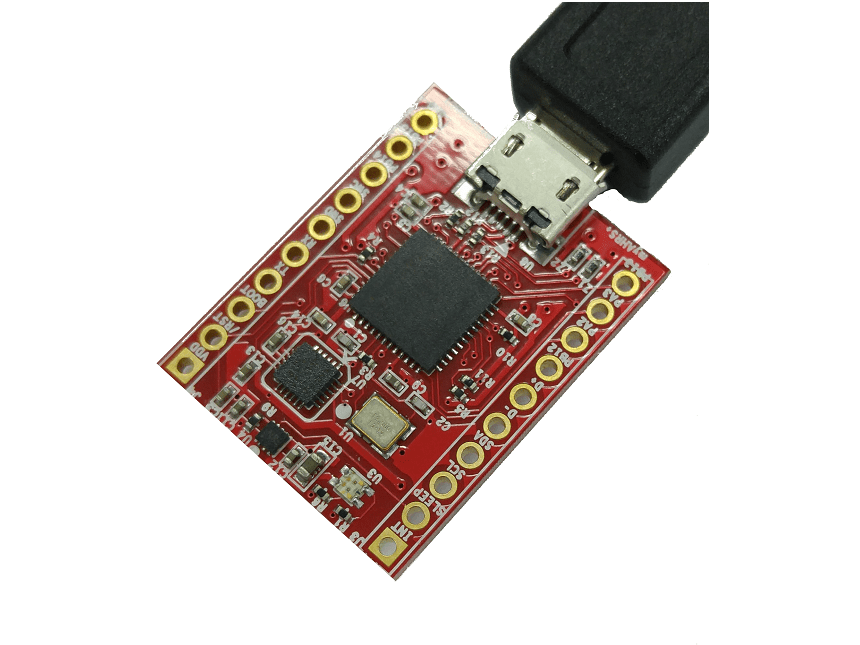
\includegraphics[width=\textwidth]{myAHRS}
        \caption{Withrobot myAHRS+ \cite{Withrobot2017}}
        \label{fig:imu_myahrs}
    \end{subfigure}
    % \hfill
    \begin{subfigure}[b]{0.4\textwidth}
        \centering
        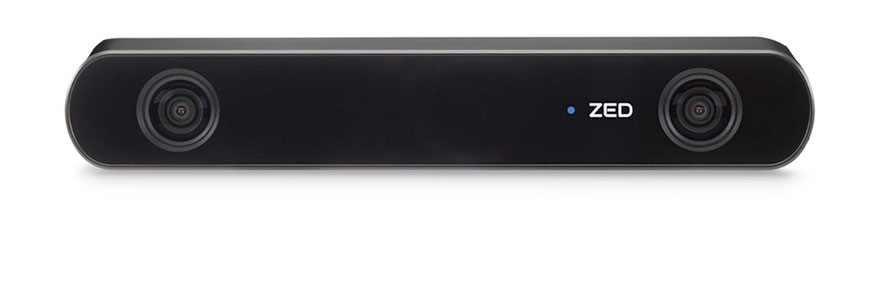
\includegraphics[width=\textwidth]{zed2i}
        \caption{Stereolabs ZED 2i camera \cite{Stereolabs2019}}
        \label{fig:imu_zed}
    \end{subfigure}
    \caption[The \glsentryplural{imu} used in the experiment]{The two \glspl{imu} which will be used for the recordings. The Stereolabs ZED 2i camera has an integrated \gls{imu}.}
    \label{fig:imus_used}
\end{figure}
Two different \glspl{imu} will be used for the experiment.\\
The first one being the Withrobot myAHRS+ (see \cref{fig:imu_myahrs}), a low-cost high performance \gls{ahrs}.
An \gls{ahrs} contains an \gls{imu} and outputs the raw measurements of the sensors, but also has an on-board processing system which estimates attitude and heading.
The myAHRS+ uses an extended Kalman filter for the estimation and outputs the estimation in quaternion form and also in Euler angles.\\
The second \gls{imu} used during the experiment is integrated in the Stereolabs ZED 2i stereo camera and is also an \gls{ahrs}.
A picture of the camera can be seen in \cref{fig:imu_zed}.
More information about the ZED 2i camera and their other integrated sensors and functionalities will be described in \cref{ssec:camera}.\\
Both sensors are connected to a computer via USB.
The specifications of each \gls{imu} can be read in \cref{tab:imu_datasheets}.
Because no information about the noise density or random walk of the myAHRS+ \gls{imu} could be found, a manual estimation of the error was done using the package \texttt{allan\_variance\_ros}~\footnote{\url{https://github.com/gaowenliang/imu_utils}}.
It analyzes the Allan variance from \gls{imu} measurement data recorded over a two-hour period, during which the \gls{imu} has not been moved.
The smaller values of the ZED 2i \gls{imu} indicate, that it is the better sensor.
\begin{table}[ht]
    \centering
    \caption{Comparison of the two used \glspl{imu} \cite{Withrobot2017, Stereolabs2019}}
    \label{tab:imu_datasheets}
    \begin{tabular}[t]{lrrc}
        \toprule
        \textbf{Property}           & \textbf{myAHRS+} & \textbf{ZED 2i \gls{imu}} & \textbf{Unit}                                               \\
        \midrule
        Accelerometer range         & $\pm16$          & $\pm8$                    & \si{g}                                                      \\
        Gyroscope range             & $\pm2000$        & $\pm1000$                 & \si{\degree\per\second}                                     \\
        Magnetometer range          & $\pm1200$        & $\pm2500$                 & \si{\micro\tesla}                                           \\
        Rate                        & \SI{100}         & \SI{400}                  & \si{\hertz}                                                 \\
        Accelerometer noise density & \SI{4.502e-3}{}  & \SI{1.148e-3}{}           & \si{\frac{\metre}{\second\squared}\frac{1}{\sqrt{\hertz}}}  \\
        Accelerometer random walk   & \SI{7.337e-5}{}  & \SI{6.458e-5}{}           & \si{\frac{\metre}{\second\cubed}\frac{1}{\sqrt{\hertz}}}    \\
        Gyroscope noise density     & \SI{1.674e-4}{}  & \SI{8.254e-5}{}           & \si{\frac{\radian}{\second}\frac{1}{\sqrt{\hertz}}}         \\
        Gyroscope random walk       & \SI{5.042e-6}{}  & \SI{1.632e-7}{}           & \si{\frac{\radian}{\second\squared}\frac{1}{\sqrt{\hertz}}} \\
        \bottomrule
    \end{tabular}
\end{table}


\subsection{\glsentryshort{lidar}}
\begin{figure}[htbp]
    \centering
    \begin{subfigure}{0.4\textwidth}
        \centering
        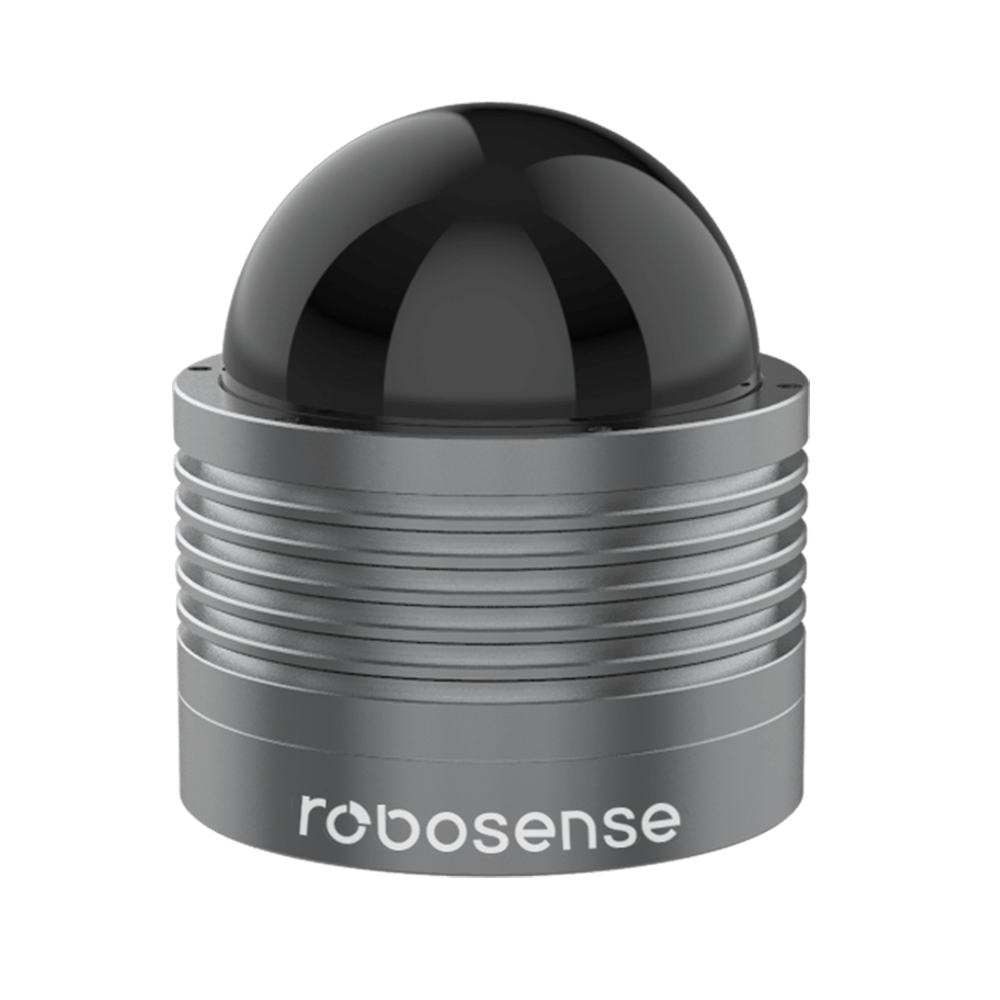
\includegraphics[width=\textwidth]{Robosense}
        \caption[The \glspl{lidar} used in the experiment]{Robosense RS-Bpearl \cite{RoboSense2020}}
        \label{fig:lidar_robosense}
    \end{subfigure}
    % \hfill
    \begin{subfigure}{0.4\textwidth}
        \centering
        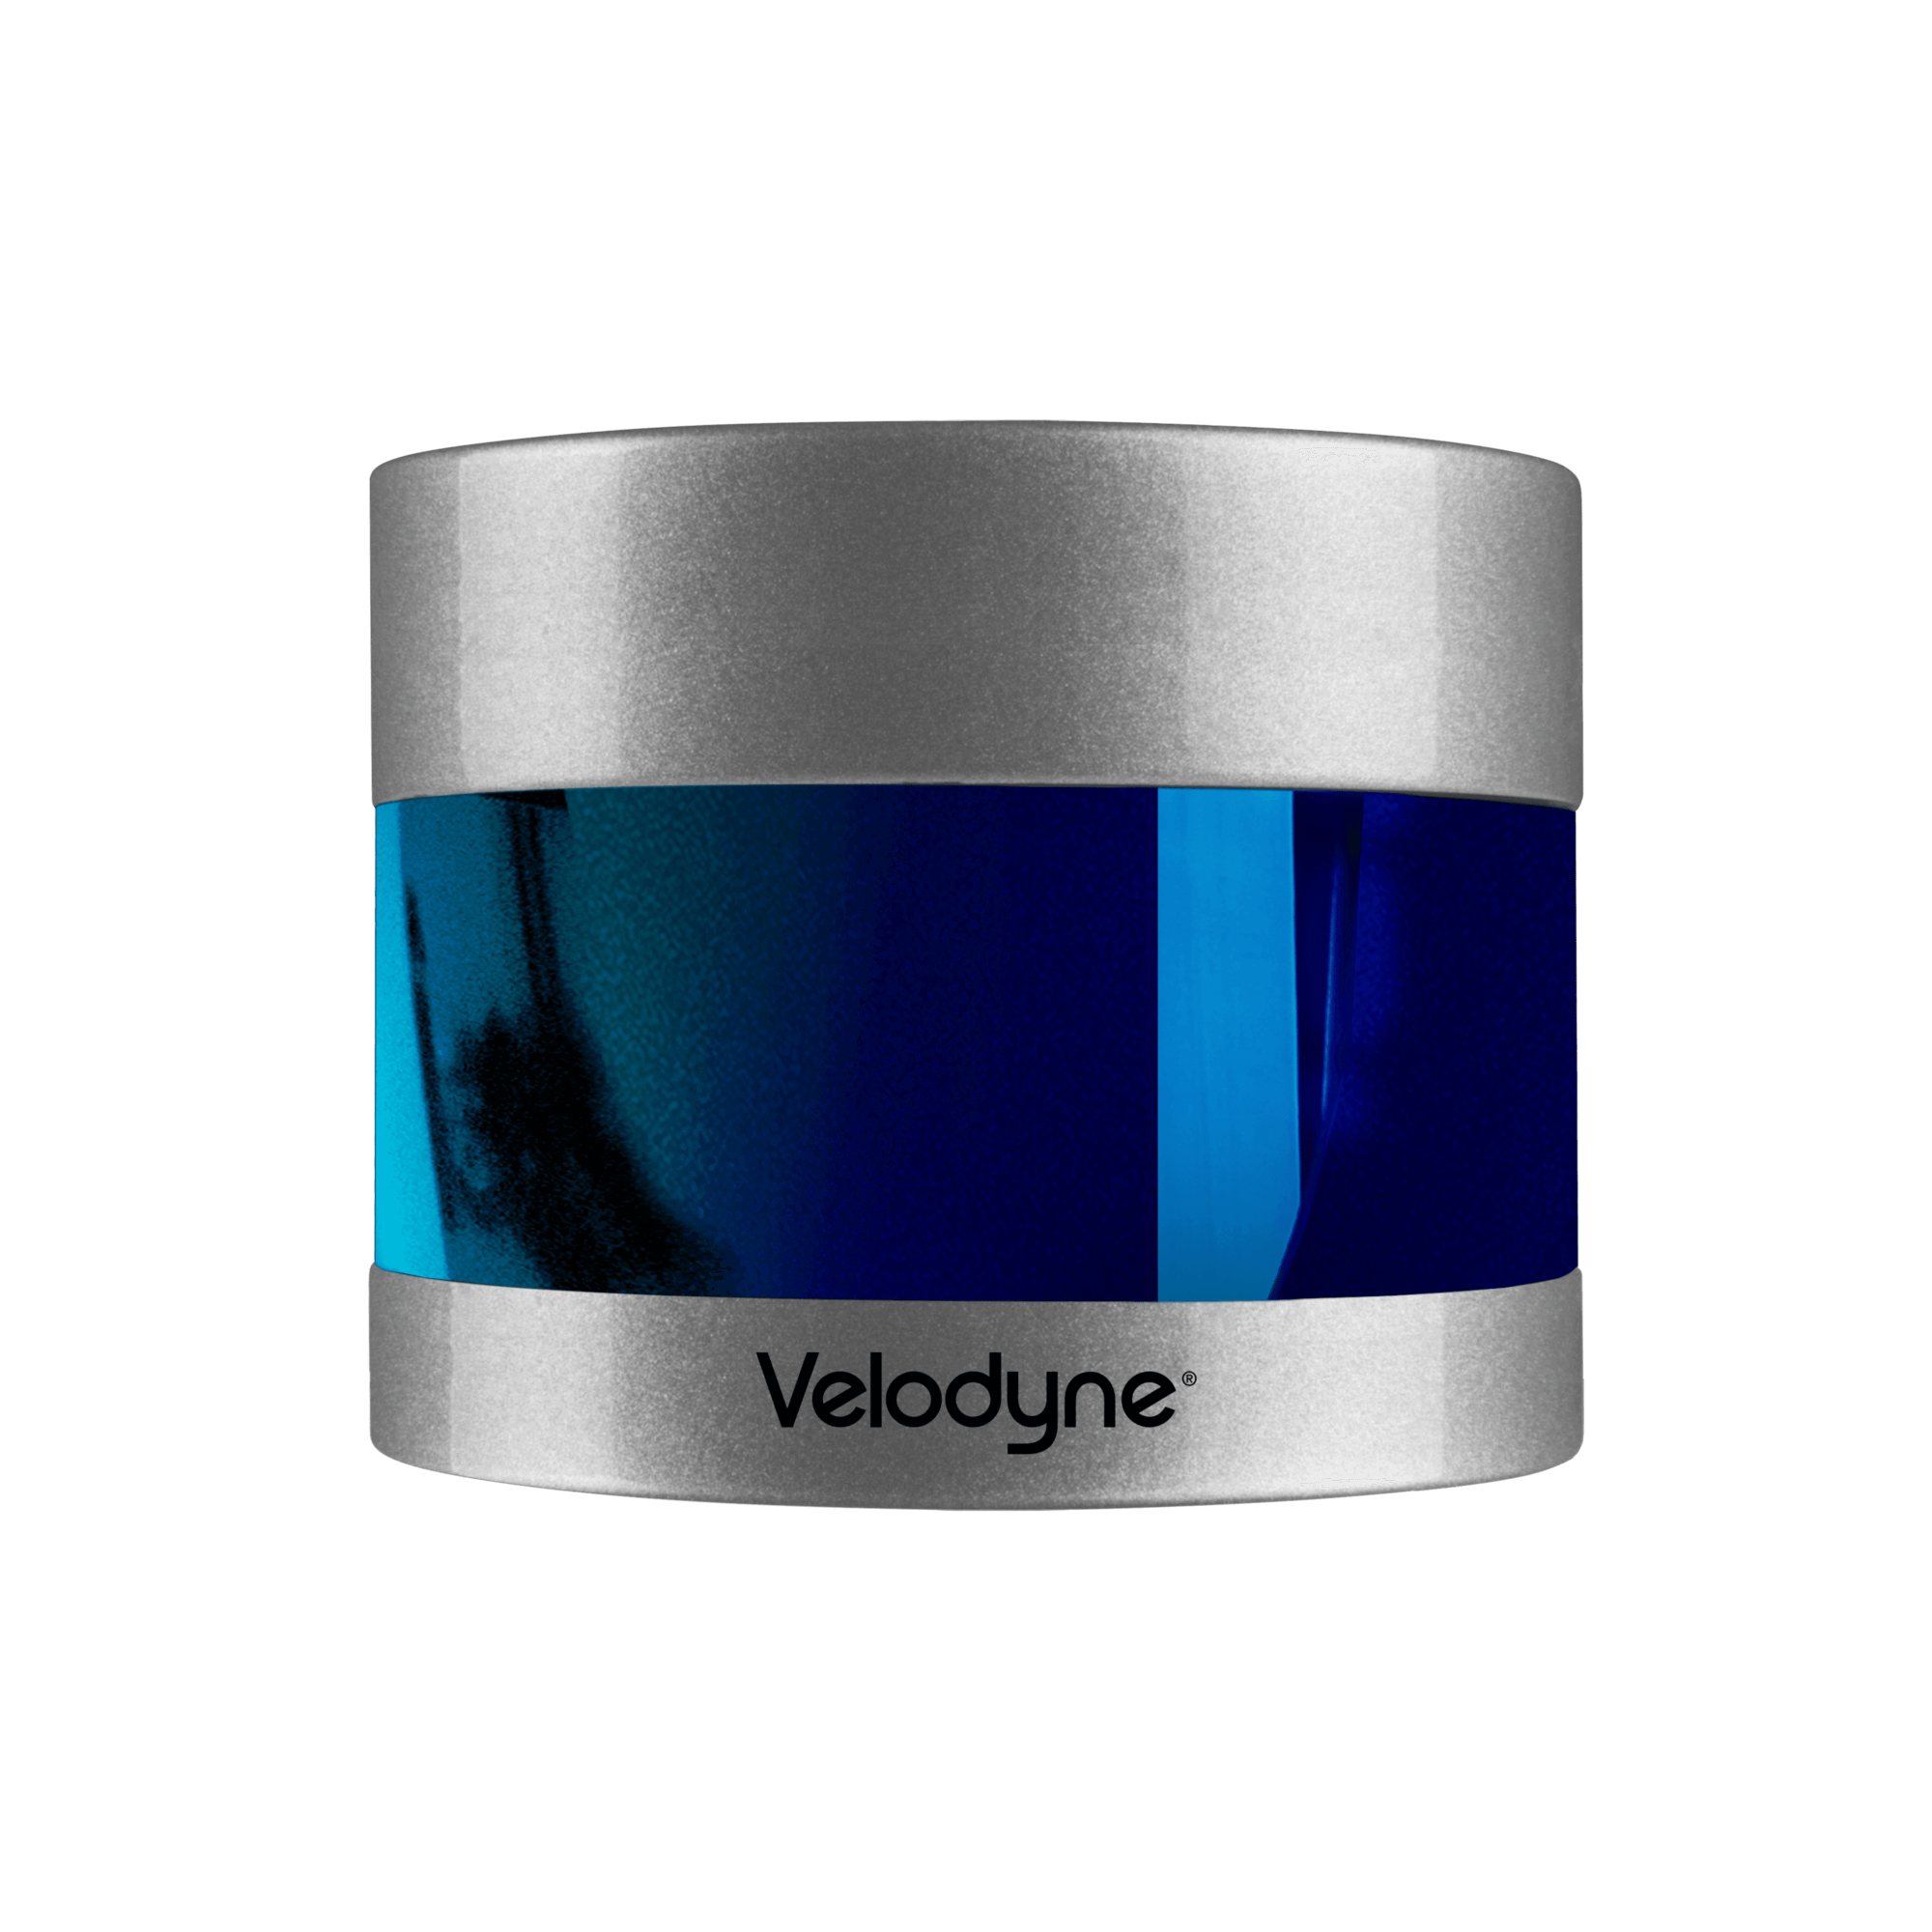
\includegraphics[width=\textwidth]{Velodyne}
        \caption{Velodyne Ultra puck \cite{Velodyne2018}}
        \label{fig:lidar_velodyne}
    \end{subfigure}
    \caption{The two \glsentryplural{lidar} which will be used for the recordings.}
    \label{fig:lidars_used}
\end{figure}
Two different \glspl{lidar} will be used during the experiment.
The RS-Bpearl and the Velodyne UltraPuck, see \cref{fig:lidars_used}.
The most relevant specifications of the two \glspl{lidar} can be seen in \cref{tab:lidar_datasheets}.
Both are mechanical \glspl{lidar} and have the same number of laser channels, but the Velodyne has a significant better vertical resolution, due to the smaller vertical \gls{fov}.
This is because the RS-Bpearl is intended to be used as near-field blind-spots detection \gls{lidar} mounted on the side where coverage is more important than resolution.
The Velodyne UltraPuck on the other hand has been specifically designed for being mounted on the roof and hence also has a greater range.\\
Both \glspl{lidar} need an external power supply and the data transfer to the PC is done via Ethernet connection.
Due to the setup of the test car it is only possible to mount one \gls{lidar} at a time.
\begin{table}[ht]
    \centering
    \caption{Comparison of the two used \acrshort{lidar}s \cite{RoboSense2020, Velodyne2018}}
    \label{tab:lidar_datasheets}
    \begin{tabular}[t]{lrrc}
        \toprule
        \textbf{Property}     & \textbf{RS-Bpearl}   & \textbf{Velodyne Ultra Puck}    & \textbf{Unit}     \\
        \midrule
        Channels              & 32                   & 32                              &                   \\
        Points per second     & 576,000              & 600,000                         & \si{}             \\
        Laser wavelength      & \SI{905}{}           & \SI{903}{}                      & \si{\nano\metre}  \\
        Frame rate            & \SIrange{10}{20}{}   & \SIrange{5}{20}{}               & \si{\hertz}       \\
        Range                 & \SI{100}{}           & \SI{200}{}                      & \si{\metre}       \\
        Range accuracy        & $\pm\SI{3}{}$        & $\pm\SI{3}{}$                   & \si{\centi\metre} \\
        Horizontal \gls{fov}  & \SI{360}{}           & \SI{360}{}                      & \si{\deg}         \\
        Vertical \gls{fov}    & \SI{90}{}            & \SI{40}{} (\SIrange{-25}{15}{}) & \si{\deg}         \\
        Horizontal resolution & \SIrange{0.2}{0.4}{} & \SIrange{0.1}{0.4}{}            & \si{\deg}         \\
        Vertical resolution   & \SI{2.81}{}          & \SI{0.33}{}                     & \si{\deg}         \\
        \bottomrule
    \end{tabular}
\end{table}


\subsection{Camera}
\label{ssec:camera}
The ZED 2i camera from Stereolabs as seen in \cref{fig:imu_zed} will be used during the experiment to record the camera image.
The camera has two horizontally displaced lenses, allowing for stereo vision and thus also depth estimation.
A barometer, temperature sensor and an \gls{imu} are integrated as well.
It also provides many more features such as 3D positional tracking, mapping, object detection and point cloud generation.\\
Because only one image is needed, only the image of the left camera is used.
The resolution is set to 1280x720 and a frame rate of 30 \gls{fps} is used.
The camera is connected to the PC through USB.



\section{Sensor Placement}
To ensure the best possible performance of the system, the sensors must be placed in a specific way.
The \gls{imu} must be placed on a rigid point of the car, such that the \gls{imu}'s position always stays the same relative to the car.
Other than that it should also be placed in the transversal center of the car to guarantee that the centripetal acceleration is not skewed towards one side when driving around a corner.
The placement of the \gls{imu} integrated in the ZED 2i camera is limited, because the camera images are needed as well.
It was placed on the roof of the car, which is sturdy enough to not be suspect to flexion, while also allowing for a good \gls{fov} for the camera.
The myAHRS+ \gls{imu} was mounted on the floor of the car trunk.\\
The \gls{lidar} is placed on top of the car, to get a greater \gls{fov}.
The pitch angle $\beta$ at which the \gls{lidar} will be mounted should be chosen such that the number of points in the area at the beginning of the ramp are maximized.
This allows for the most accurate distinction between planes of different inclination angles.
Because the distance to the ramp is not constant due to the movement of the car, the optimization can only be done for a specific distance.
The coordinates at which the lasers hit the ground and ramp depend on the height of the \gls{lidar} $h_\mathrm{l}$, the distance to the ramp $d$, the angle of the ramp \gls{ramp_ang}, the angle $\beta$ at which the \gls{lidar} has been mounted on the car and finally on the vertical resolution $\epsilon$ and \gls{fov} of the \gls{lidar}.
A visualization of the different variables can be seen in \cref{fig:tikz_lidar_mount}.
\begin{figure}[htb]
    \centering
    \documentclass[12pt]{standalone}
\usepackage{tikz}
\usepackage{tikz-dimline}		% Dimension (measure) lines for TikZ
\usetikzlibrary{angles, calc, decorations.pathmorphing, quotes, spy}

\begin{document}
\begin{tikzpicture}[scale=0.85, spy using outlines={black, rectangle, magnification=3, width=5cm, height=1.2cm, connect spies}]
        % Define/Calc ramp parameters
        % Ramp length
        \def\rl{5};
        % Ramp angle [deg]
        \def\ra{15};
        % Ramp height
        \def\rh{{tan(\ra)*\rl}};
        % Distance of measurement line
        \def\dd{.4cm}

        % RAMP
        % Define the points
        % Left point
        \coordinate (A) at (0,0);
        % Lower right point
        \coordinate (B) at ($(A) + (\rl,0)$);
        % Upper right point
        \coordinate (C) at ($(B) + (0,\rh)$);

        % Draw and fill ramp
        \filldraw[draw=black, fill=lightgray!25] (A) -- (B) -- (C) -- cycle;
        % Draw ramp angle
        \path (A) -- (B)
        pic[draw, ->, angle radius=40pt,
                        angle eccentricity=0.75, "$\alpha$"]{angle=B--A--C};

        % Most left point at ground level
        \coordinate (D) at ($(A) + (-10,0)$);
        % Ground line
        \draw [thick] (D) -- (A) -- (C);


        % CAR
        \begin{scope}[scale=0.7]
                % Car height
                \def\ch{2}
                % Car length
                \def\cl{5}
                % Car body height
                \def\bh{\ch*0.65}
                % Roof length
                \def\rl{\cl*0.6}
                % Roof height
                \def\rh{\ch*0.35}
                % Anchor point of car body (lower left)
                \coordinate (b) at ($(D) + (0,0.5)$);
                % Offset to roof and wheels
                \coordinate (r) at ($(b) +(\cl*0.17,\ch*0.65)$);
                \coordinate (w) at ($(b) + (\cl*0.25,0)$);

                % Body
                \draw[black, fill=black!17, rounded corners=1.2ex, very thick]
                (b) -- ++(0,\bh) -- ++(\cl*1/5,0) --  ++(\cl*3/5,0) -- ++(\cl*1/5,-\bh*0.25)
                -- ++(0, -\bh*0.75) -- (b) -- cycle;
                % Roof
                \draw[very thick, rounded corners=0.5ex, fill=black!20!blue!20!white,thick]
                (r) -- ++(0.2*\rl,\rh) -- ++(0.5*\rl,0) -- ++(0.3*\rl,-\rh) -- (r);
                \draw[thick] (r)++(\rl*0.6,0) -- ++(0,\rh);

                % Wheels
                \draw[draw=black,fill=gray!50,thick] (w) circle (.5);
                \draw[draw=black,fill=gray!50,thick] (w) ++(\cl*0.55,0) circle (.5);
                % Inner wheels
                \draw[draw=black,fill=gray!80,semithick] (w) circle (.35);
                \draw[draw=black,fill=gray!80,semithick] (w) ++(\cl*0.55,0) circle (.35);

                % Lidar
                % Lidar pitch angle
                \def\lpa{10};
                \draw[black, fill=gray!50] ($(r) + (\cl*0.40,\rh)$) coordinate (le) arc(-\lpa*2:180:0.4) --cycle;

                % Car middle point
                \coordinate (m) at (\cl*0.5, \bh*0.5);
                % Lidar middle point
                \coordinate (lm) at ($(le) + (-0.39,0.25)$);
                \filldraw[red] (lm) circle(.1);
                \coordinate (idk) at ($(A)!0.4!(C)$);

                % Laser lines
                \draw[->,color=red,very thin,decorate,decoration={snake,amplitude=.2mm,segment length=1mm,post length=1mm}] (lm) -- (A)
                pic[draw, black, ->, thin, angle radius=100pt, angle eccentricity=0.95,
                                "$\epsilon$"]{angle=A--lm--idk};
                \draw[->,color=red,very thin,decorate,decoration={snake,amplitude=.2mm,segment length=1mm,post length=1mm}] (lm) -- ($(A)!0.4!(C)$);
                \draw[->,color=red,very thin,decorate,decoration={snake,amplitude=.2mm,segment length=1mm,post length=1mm}] (lm) -- ($(A)!1!(C)$)
                pic[draw, black, ->, thin, angle radius=120pt, angle eccentricity=0.95,
                                "$2\epsilon$"]{angle=A--lm--C};


                % lidar mount angle
                % Length of angle helper line
                \def\hl{4};
                \def\hll{1.8};
                \coordinate (bleb) at ($(lm) + (\hl+1, 0)$);
                \coordinate (blab) at ($(lm) + (\hl, -{tan{\lpa}*\hl})$);
                \coordinate (blub) at ($(lm) + (-\hll, 0)$);
                \coordinate (blob) at ($(lm) + (-\hll, +{tan{\lpa}*\hll})$);
                \draw[draw=gray, very thin] (blub) -- (lm) -- (blob)
                pic[draw, black, thin, <-, angle radius=30pt,
                                angle eccentricity=0.82, "\tiny $\beta$"]{angle=blob--lm--blub};
                \draw[draw=gray, very thin] (bleb) -- (lm) -- (blab)
                pic[draw, black, thin, <-, angle radius=68pt,
                                angle eccentricity=0.9, "$\beta$"]{angle=blab--lm--bleb};
                \path (bleb) -- (lm) -- (A)
                pic[draw, <-, thin, angle radius=84pt,
                                angle eccentricity=0.9, "$\gamma$"]{angle=A--lm--bleb};

        \end{scope}

        % \filldraw[green] (idk) circle(.2);
        \dimline[extension start length=\dd, extension end length=\dd+1.9cm] {($(lm)+(0,\dd)$)}{($(lm -| A)+(0,\dd)$)}{$d$};
        % \dimline[extension start length=-\dd, extension end length=-\dd] {($(A)+(0,-\dd)$)}{($(B)+(0,-\dd)$)}{$l_\mathrm{r} $};
        \dimline[extension start length=-\dd, extension end length=-\dd, label style={sloped=false}] {($(B)+(\dd,0)$)}{($(C)+(\dd,0)$)}{$h_\mathrm{r}$};
        \dimline[extension start length=\dd, extension end length=\dd+1.7cm, label style={sloped=false}] {($(D)+(-\dd,0)$)}{($(lm -| D)+(-\dd,0)$)}{$h_\mathrm{l} $};

        % \dimline[extension start length=\dd, extension end length=-\dd] {($(idk)+(\dd,0)$)}{($(idk)+(\dd,-0.53)$)}{};
        % \dimline[extension start length=0, extension end length=0, label style={right, fill=none, sloped=false}] {(idk)}{($(idk)+(0,-0.53)$)}{$h_\mathrm{w}$};
        \dimline[extension start length=-\dd, extension end length=-\dd] {($(A)+(0,-\dd)$)}{($(idk)+(0,-\dd-15)$)}{$d_\mathrm{w} $};
        \dimline[extension start length=\dd, extension end length=\dd] {($(A)+(0.05,-\dd+\dd+34.3)$)}{($(idk)+(0.05,\dd)$)}{$l_\mathrm{w} $};

        % \spy[black] on ($(lm) + (-0.42, 0)$) in node at (3,4);
        \spy on ($(lm) + (-0.25, 0)$) in node at ($(lm) + (-0.3, 1.5)$);

\end{tikzpicture}
\end{document}
    \caption[\acrshort{lidar} placement on the car]{Calculation of the best mounting angle of the \acrshort{lidar} on the car. Variable description in \cref{tab:lidar_mount}.}
    \label{fig:tikz_lidar_mount}
\end{figure}
The coordinates at which the laser lines of the \gls{lidar} hit the ground can be calculated in the following way.\\
The angle $\kappa$ between the plane parallel to the ground at \gls{lidar} height and each laser wave is defined as
\begin{equation}
    \kappa = \beta - i\epsilon
\end{equation}
with $i \in [0,1,2,\dots,n]$ being the laser channel ID starting from the lowest opening angle and going to the highest and $n$ being the number of laser channels.
On flat ground the distance at which the laser waves hit the ground can be calculated by
\begin{equation}
    d_\mathrm{hit,ground}  = \tan(\ang{90} - \kappa) h_\mathrm{l}.
    \label{eq:ground_points}
\end{equation}
With a ramp, the assumption from \cref{eq:ground_points} does not hold anymore.
The light does not travel as far.
The height above ground, when the light is at the beginning of the ramp can be calculated by
\begin{equation}
    h_\mathrm{w,start} = h_\mathrm{l} - d\tan(\kappa).
\end{equation}
The distance $l_\mathrm{w}$ which the light travels from the beginning of the ramp to the contact point with the ramp can be calculated using the law of sines
\begin{align}
    l_\mathrm{w} & = \frac{h_\mathrm{w,start} }{\sin(\gls{ramp_ang} + \kappa)} \sin(\ang{90} - \gls{ramp_ang}) \nonumber \\
                 & = -\frac{h_\mathrm{w,start} }{\sin(\gls{ramp_ang} + \kappa)} \cos(\gls{ramp_ang}).
\end{align}
The traveled distance along the x-axis from the start of the ramp to the contact point is then
\begin{align}
    d_\mathrm{w} & = l_\mathrm{w} \sin(\ang{90} - 2\gls{ramp_ang} - \kappa) \nonumber \\
                 & = -l_\mathrm{w} \cos(2\gls{ramp_ang} + \kappa).
\end{align}
Putting everything together, the total x distance from the \gls{lidar} to the contact point on the ramp can be calculated by
\begin{align}
    d_\mathrm{hit,ramp} & = d + d_\mathrm{w}                                                                                    \nonumber               \\
    d_\mathrm{hit,ramp} & = d + \frac{h_\mathrm{l} - d\tan(\kappa)}{\sin(\gls{ramp_ang} + \kappa)} \cos(\gls{ramp_ang}) \cos(2\gls{ramp_ang} + \kappa).
    \label{eq:final_equation}
\end{align}
Using \cref{eq:ground_points} and \cref{eq:final_equation} and optimizing $\beta$ such that the number of points in the area at the start of the ramp are maximized, the optimal mounting pitch angle $\beta$ for the two \glspl{lidar} has been found with $\beta_\mathrm{velodyne} = \ang{0}$ and $\beta_\mathrm{robos} = \ang{20}$.
The optimization was done for a distance of \SI{10}{\metre} to the ramp.
The angle between the two \glspl{lidar} differs due to the different starting opening angle of \SI{-25}{\degree} and \SI{0}{\degree} for the Velodyne and Robosense respectively, as well as due to the different vertical resolution.
A detailed description of all the variables used for the calculation can be found in \cref{tab:lidar_mount}.
\begin{table}[htb]
    \centering
    \caption{Variables used to calculate the optimal mounting angle of the \gls{lidar}.}
    \label{tab:lidar_mount}
    \begin{tabular}[t]{clc}
        \toprule
        \textbf{Variable} & \textbf{Description}                                   & \textbf{Unit} \\
        \midrule
        $h_\mathrm{l} $   & \gls{lidar} height above ground                        & \si{\metre}   \\
        $d$               & Distance to ramp                                       & \si{\metre}   \\
        $h_\mathrm{r}$    & Height of ramp                                         & \si{\metre}   \\
        $l_\mathrm{w}$    & Light travel distance from ramp start to contact point & \si{\metre}   \\
        $d_\mathrm{w}$    & Distance from ramp start to contact point              & \si{\metre}   \\
        $\gls{ramp_ang}$  & Ramp angle                                             & \si{\deg}     \\
        $\beta$           & \gls{lidar} mount angle                                & \si{\deg}     \\
        $\kappa$          & Laser line angle                                       & \si{\deg}     \\
        $\epsilon$        & \gls{lidar} vertical resolution                        & \si{\deg}     \\
        $n$               & Number of laser channels                               &               \\
        \bottomrule
    \end{tabular}
\end{table}


\section{Data Recording}
All the sensors are connected to a PC in the car, located in the booth.
A notebook is connected to the PC using a \gls{ssh} connection and is used to start the different sensor streams.
For the communication between the PC and sensors and the recording of the sensor data the \gls{ros} framework is used.
Each sensor publishes its data to a specific topic, which can be subscribed to.
While \gls{ros} allows for real-time running of nodes it is also possible to record all sensor streams and store them in a rosbag.
A rosbag contains the serialized message data and can later be used as a dataset.
The rosbag can be played back in \gls{ros}, simulating the same conditions as during the recording, by publishing the same topics again which were initially subscribed to during the recording.
The different algorithms can then be tested and perhaps improved, without having to physically do the test drive again.


\section{Car}
\label{sec:car}
The car used for the recordings is an eGolf 2017.
Being an electric car it provides better vibration properties than a car with an internal combustion engine, which means that the \gls{imu} measurements are less influenced by external noise.
The car has built in wheel speed sensors, which only provide a signal if used in a special driving mode, in which the output power of the motor is limited.
In this mode, the maximum speed is capped at \SI{5}{\kilo\metre\per\hour} and the torque is limited, such that is not possible to drive a ramp all the way up.
The car can only make it about halfway up.
Because of that, the normal mode was used to drive between different levels.
Before driving down, the mode was switched again to also provide the wheel speed measurements.
A picture of the car with the mounted \gls{lidar} and ZED 2i camera can be found in \cref{fig:eGolf}.
\begin{figure}[htb]
    \centering
    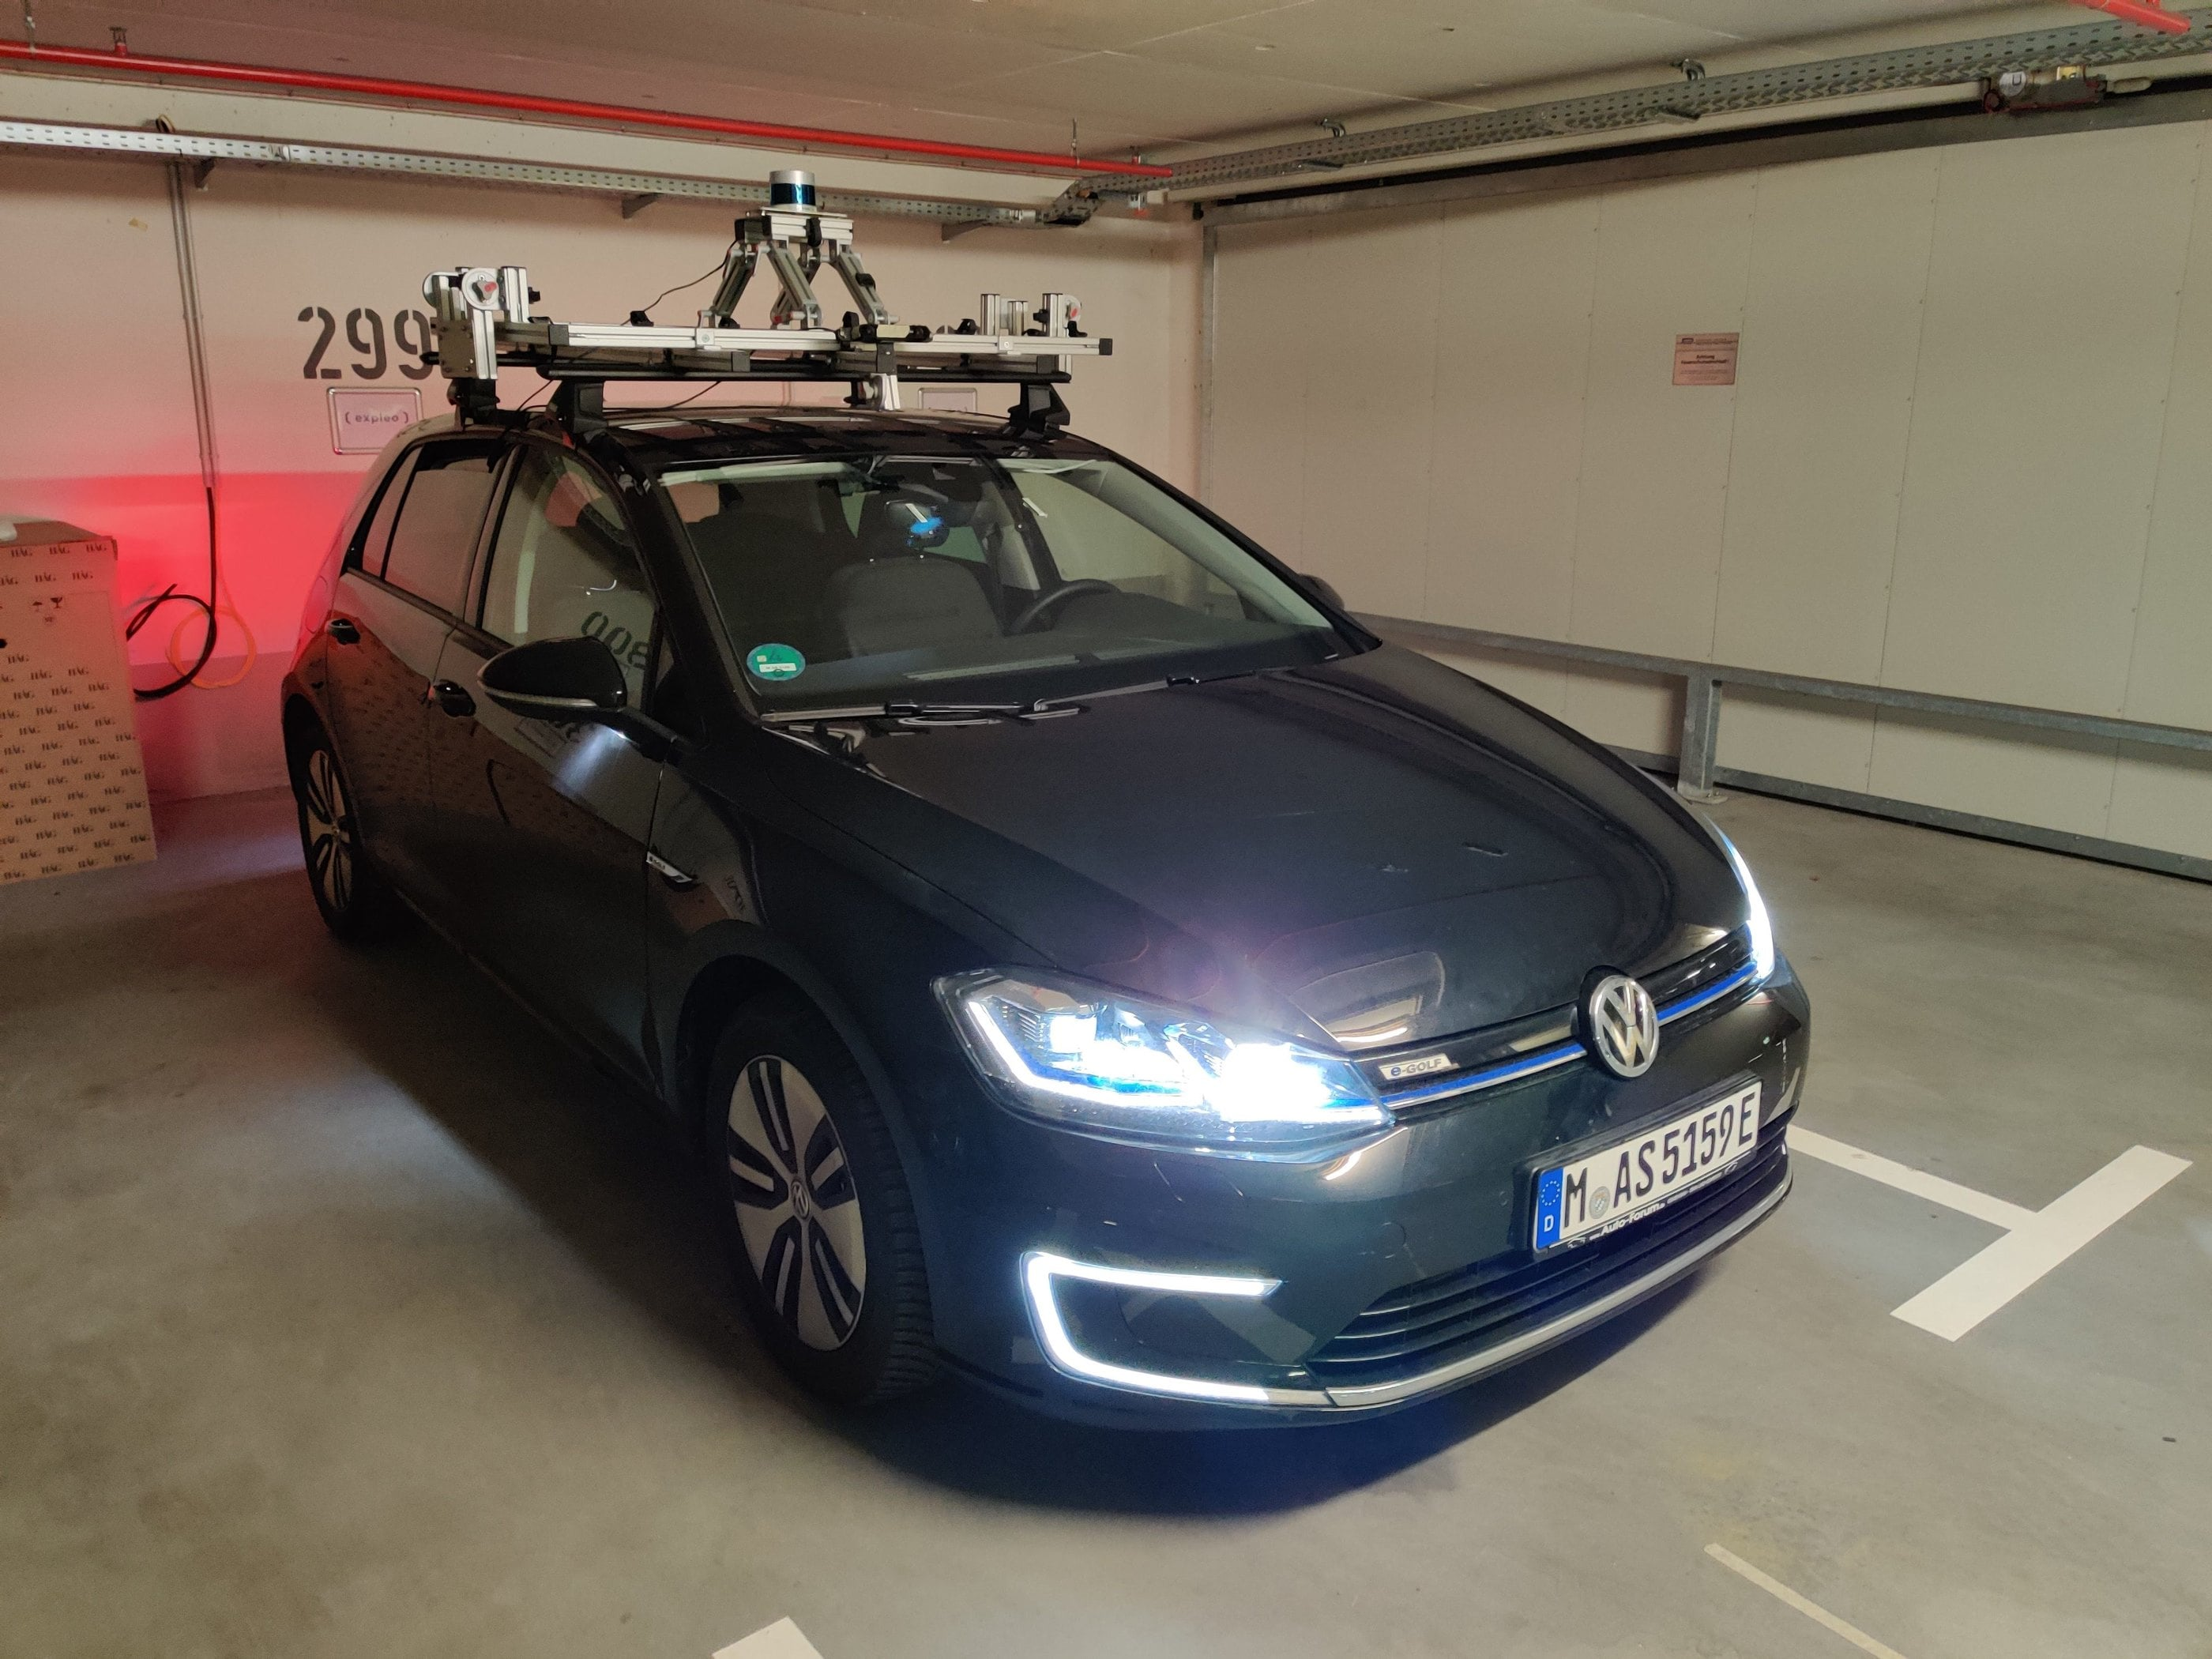
\includegraphics[trim={0, 5cm, 0, 5cm}, clip, width=0.6\linewidth]{eGolf}
    \caption[Car with mounted sensors]{The car used for the recordings with the full sensor setup mounted on the roof.}
    \label{fig:eGolf}
\end{figure}



\section{Garage}
\label{sec:garage}
To prevent an overfitting of the model it is important to have different test scenarios.
The garage in which the car is normally parked has different types of ramps, which are shown in \cref{fig:all_ramps}.
The properties of each ramp are described in \cref{tab:ramp_properties}.
The values were measured by inspecting the point cloud generated by the \gls{lidar}.
The width of the ramp is measured between the side wall and the railing, and not between the two curbsides.
Because the ramps do not have a constant angle, because the change of the angle gradually increases, decreases and then increases again, the average angle of the ramps is used.
\begin{figure}[htb]
    \begin{subfigure}{.24\linewidth}
        \centering
        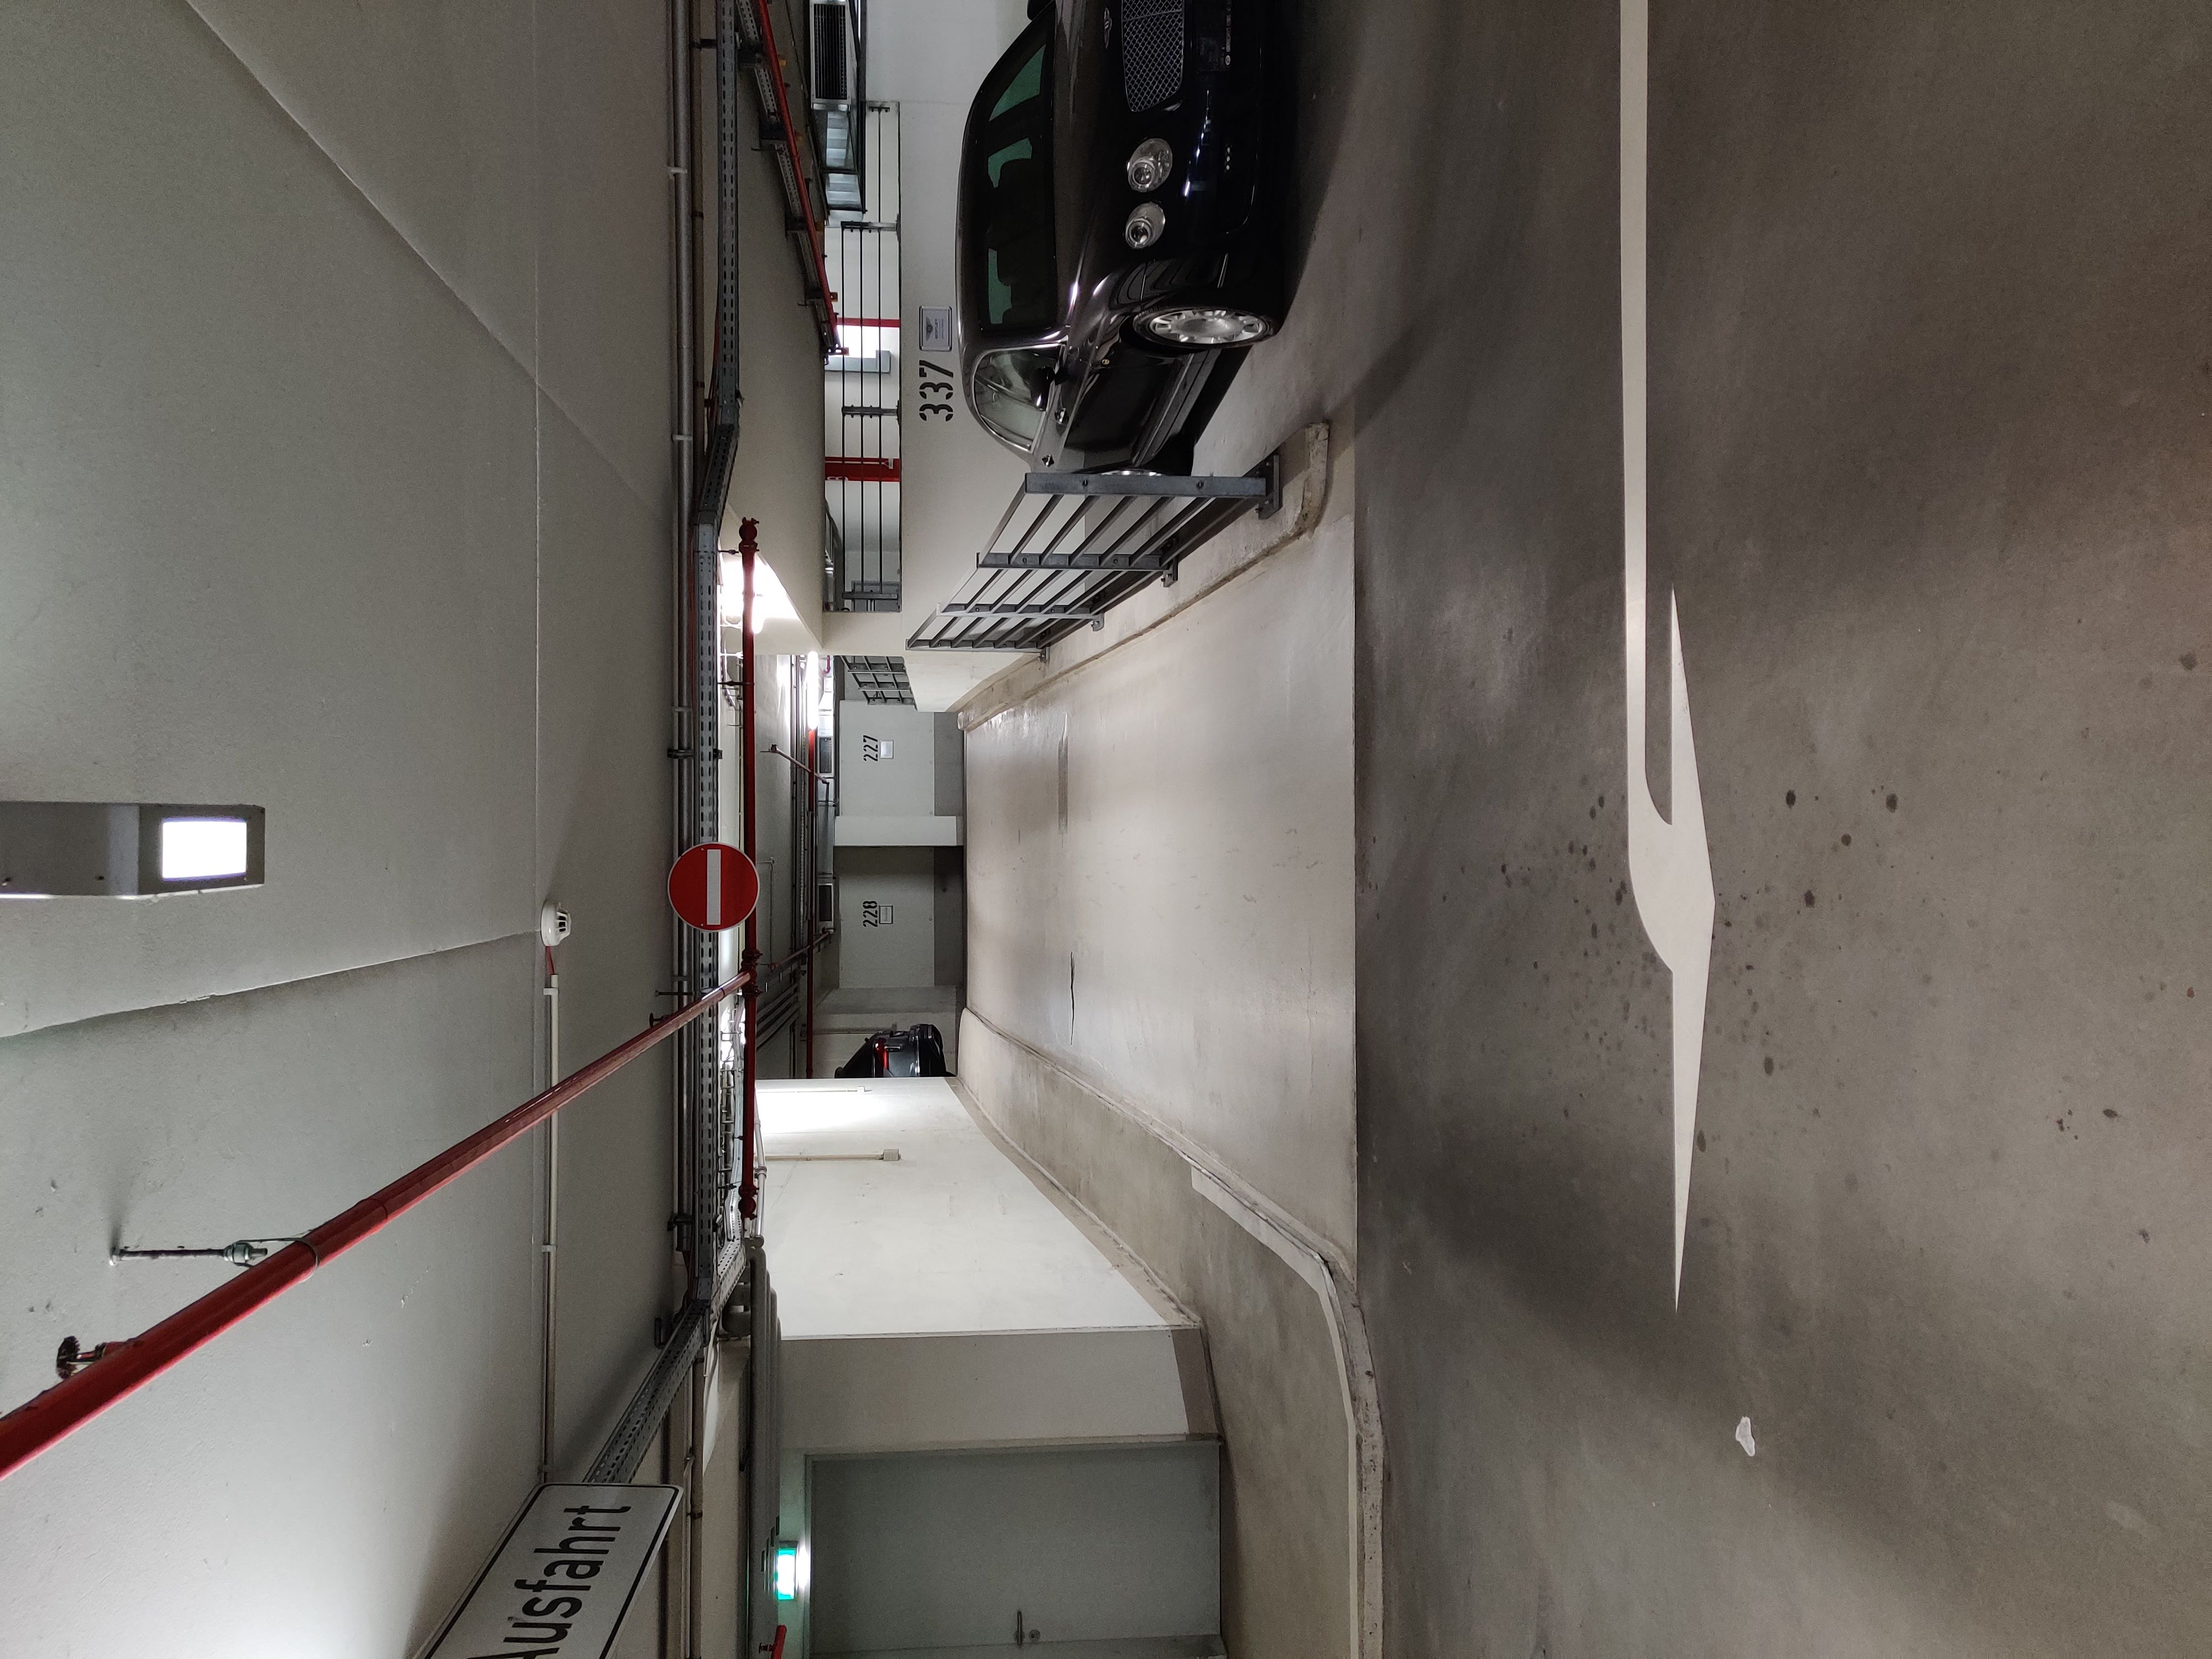
\includegraphics[angle=-90, width=1\linewidth]{RampA.jpg}
        \caption{}
    \end{subfigure}
    \hfill
    \begin{subfigure}{.24\linewidth}
        \centering
        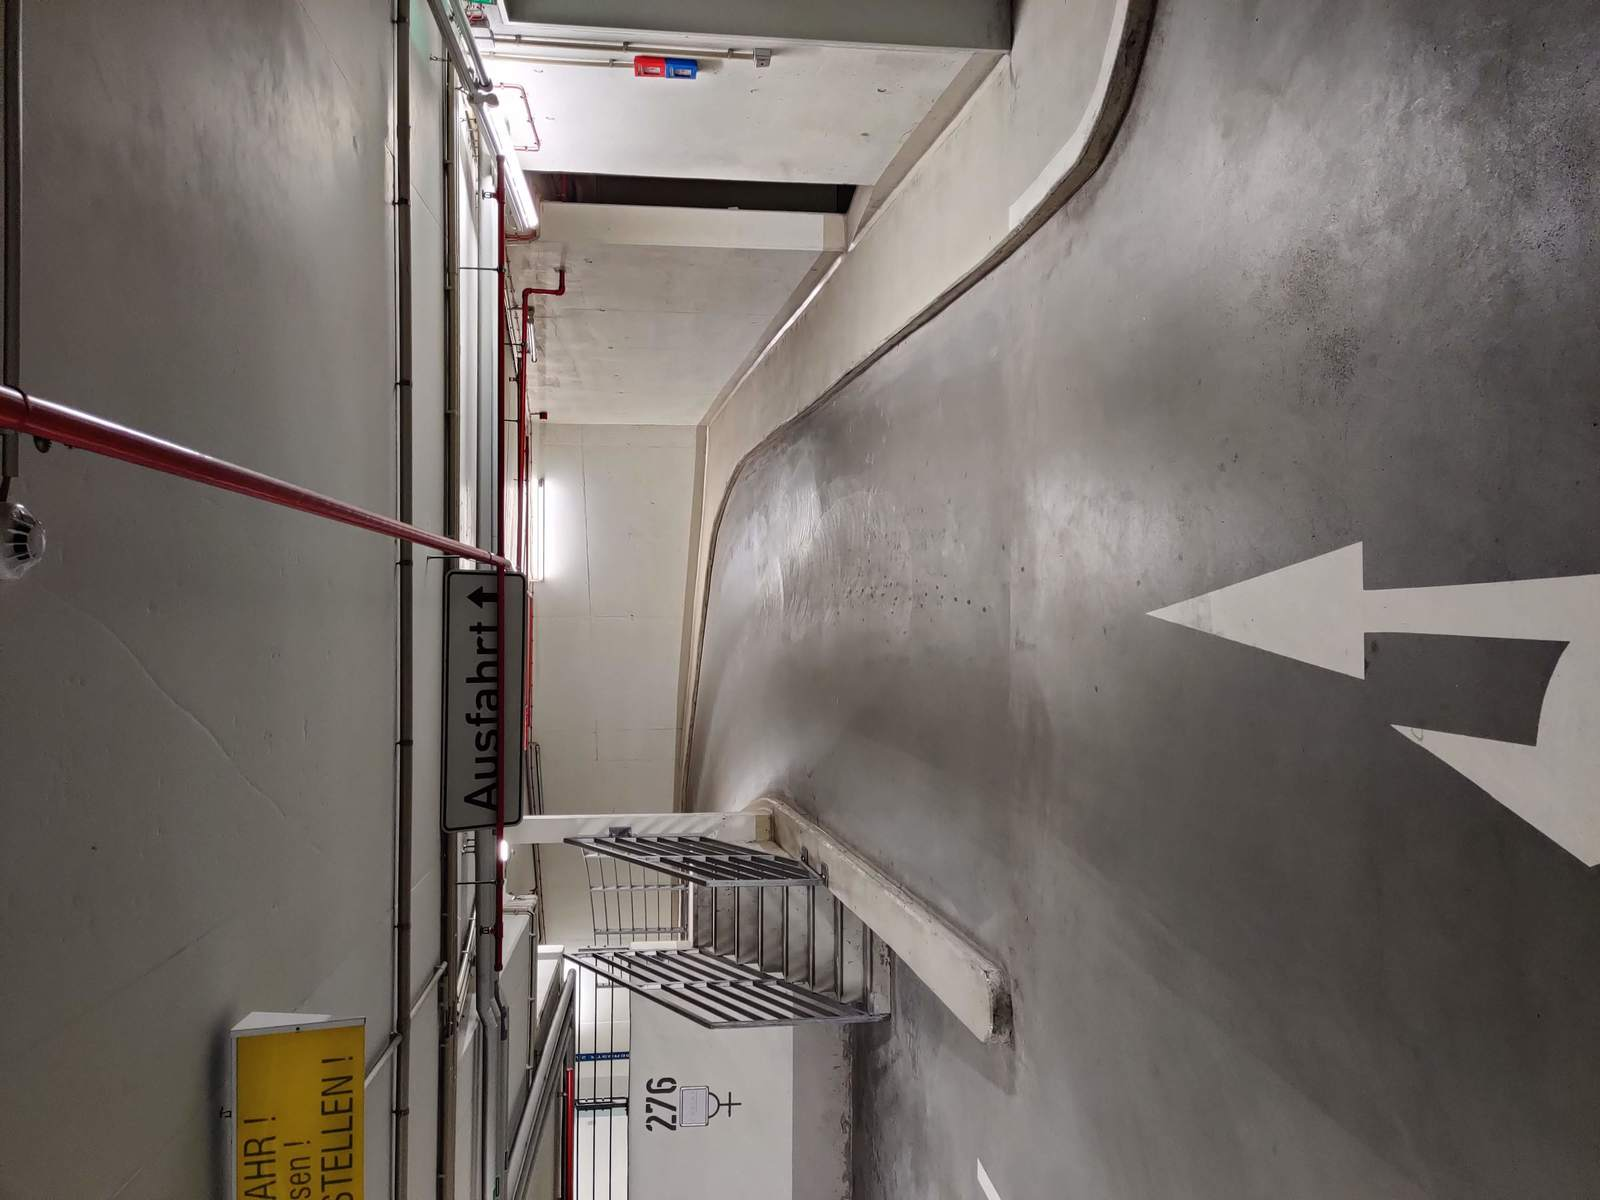
\includegraphics[angle=-90, width=1\linewidth]{RampB.jpg}
        \caption{}
    \end{subfigure}
    \hfill
    \begin{subfigure}{.24\linewidth}
        \centering
        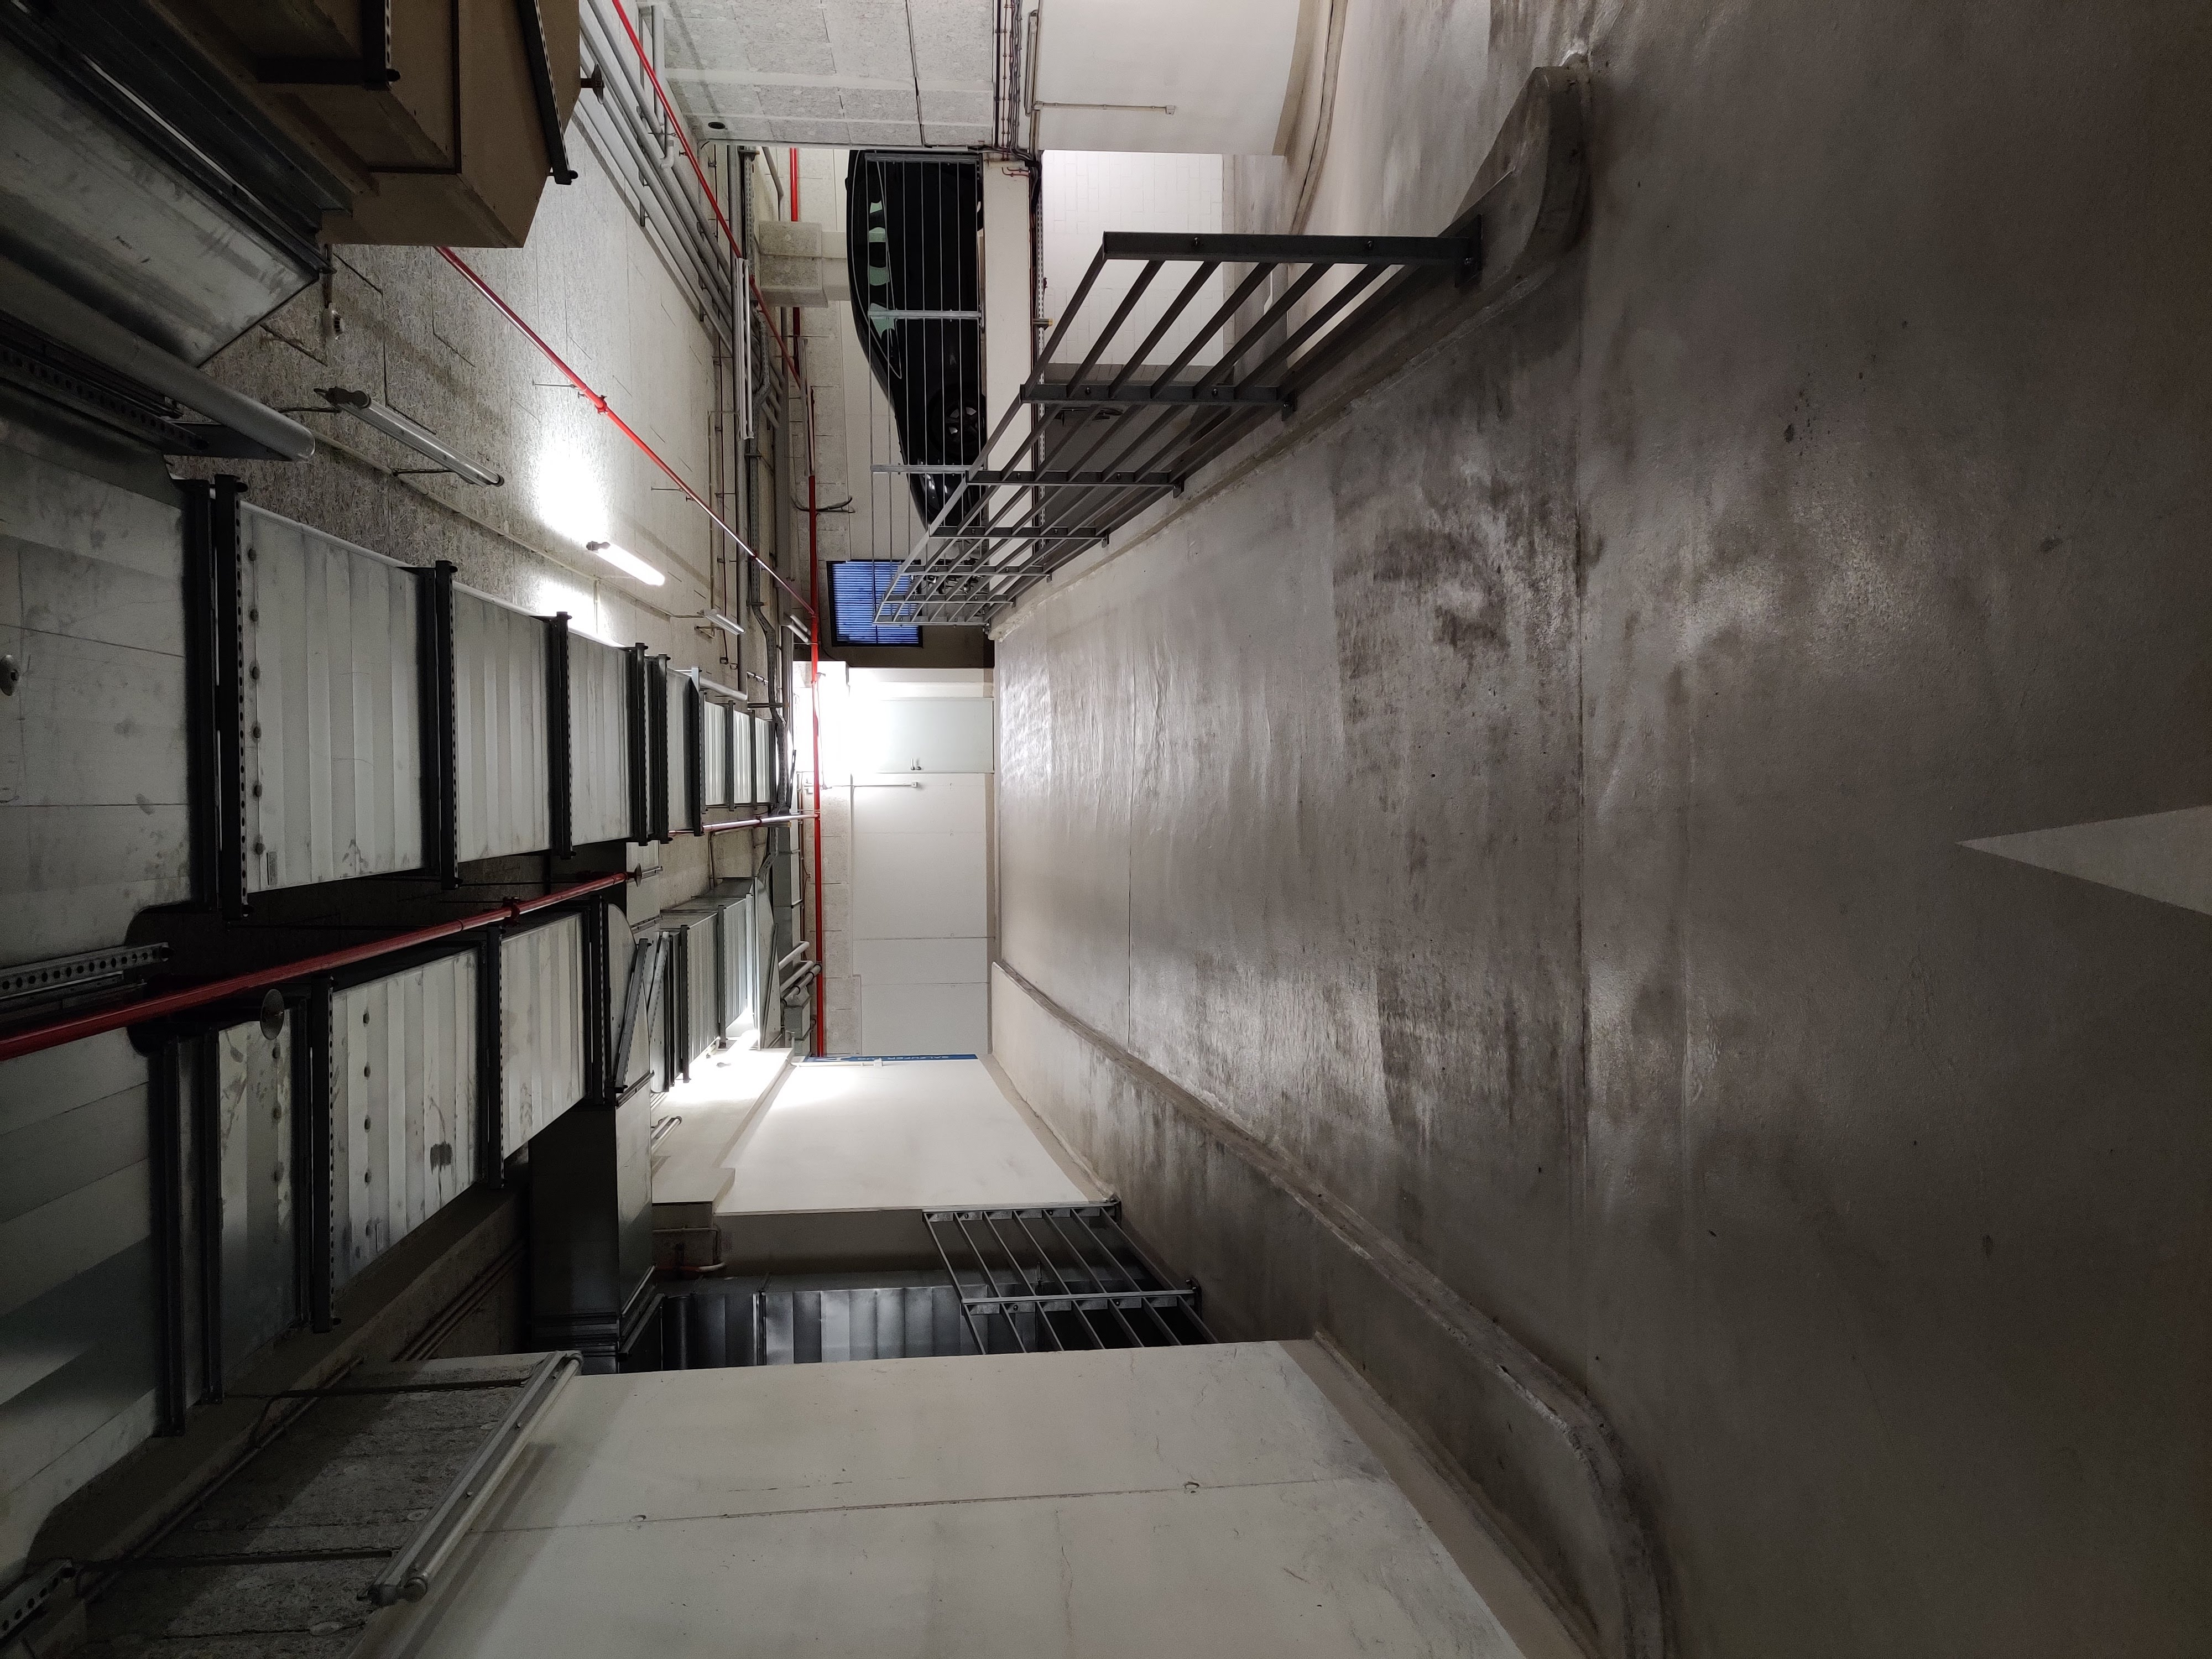
\includegraphics[width=1\linewidth]{RampC.jpg}
        \caption{}
    \end{subfigure}
    \hfill
    \begin{subfigure}{.24\linewidth}
        \centering
        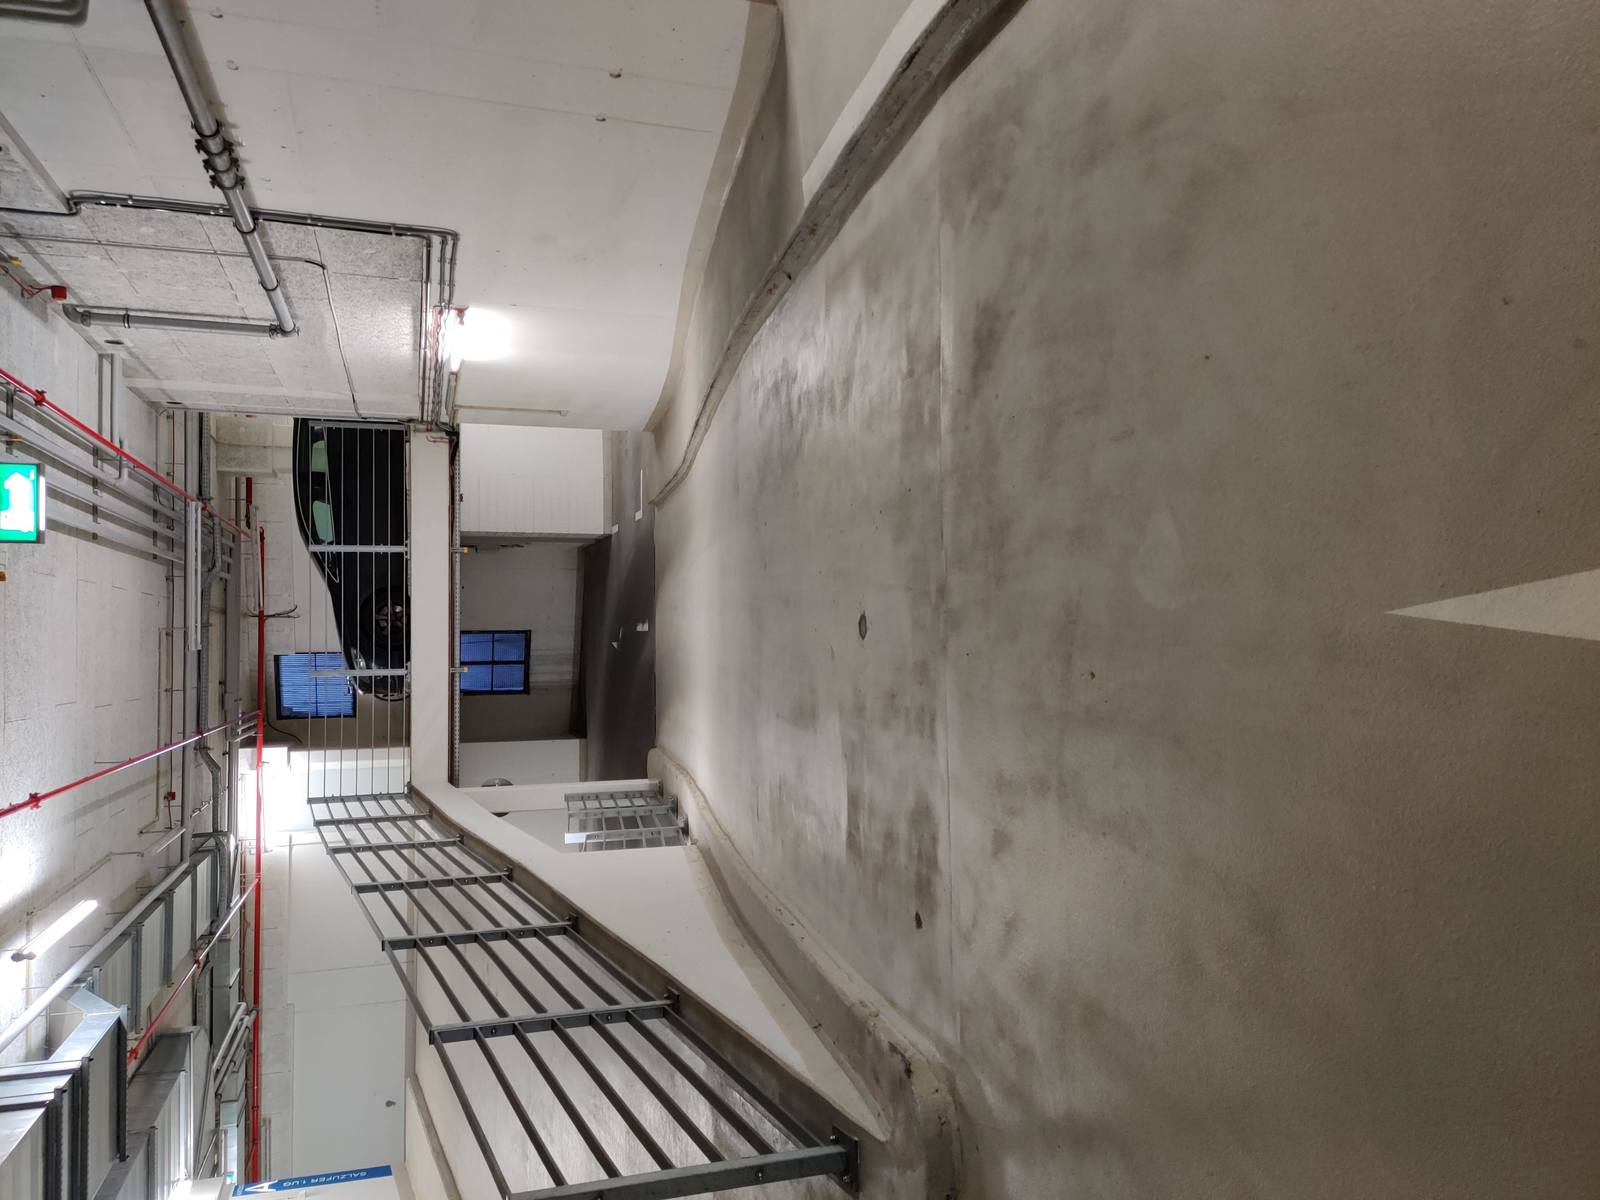
\includegraphics[angle=-90, width=1\linewidth]{RampD.jpg}
        \caption{}
    \end{subfigure}
    \caption[Ramps of the garage]{On the ramps A, B and C the car will be driven up. On the ramp D as well as also on the ramp A the car will be driven down.}
    \label{fig:all_ramps}
\end{figure}
\begin{table}[htb]
    \centering
    \caption[Measured ramp properties]{The measured ramp properties.}
    \label{tab:ramp_properties}
    \begin{tabular}[t]{cSSS}
        \toprule
        \textbf{Ramp} & {\textbf{Angle} [\si{\degree}]} & {\textbf{Width} [\si{\metre}]} & {\textbf{Length} [\si{\metre}]} \\
        \midrule
        A             & 7.2                             & 3.94                           & 11.97                           \\
        B             & 6.5                             & 3.96                           & 14.15                           \\
        C             & 7.4                             & 3.90                           & 11.85                           \\
        D             & -7.3?                           & 3.85                           & 11.89                           \\
        \bottomrule
    \end{tabular}
\end{table}
\itodo{Add curb ramp width}
\chapter{Methods}
\label{ch:Methods}
In this chapter various methods using different sensors to estimate the car's pitch angle and thus the ramp angle, as well as other properties of the ramp, such as the width and length, will be described.
The problem definition is discussed in \cref{sec:road_grade_definition}.
Before being able to use the sensor measurements, a coordinate frame transformation to the device frame is necessary.
This problem is described in \cref{sec:coordinate_frames}.
In \cref{sec:methods_imu} multiple methods to estimate the car's pitch angle using an \gls{imu} are described.
The angle is then used to identify a ramp.
A novel method using a \gls{lidar} sensor will be presented in \cref{sec:methods_lidar}.
It tracks the distance to the ramp and estimates the angle, width and length of the ramp.
Finally, a ramp detection algorithm using a camera and a trained neural network will be presented in \cref{sec:methods_camera}.


\section{Road grade definition}
\label{sec:road_grade_definition}
\begin{figure}[htb]
	\centering
	\documentclass[11pt]{standalone}
\usepackage{tikz}
\usetikzlibrary{angles, calc, decorations.pathmorphing, quotes, spy}

\begin{document}
\begin{tikzpicture}[scale=.88]
    % Define/Calc ramp parameters
    % Ramp length
    \def\rl{10};
    % Ramp angle [deg]
    \def\ra{15};
    % Ramp height
    \def\rh{{tan(\ra)*\rl}};

    % RAMP
    % Define the points
    \coordinate (A) at (0,0);
    \coordinate (B) at ($(A) + (\rl,0)$);
    \coordinate (C) at ($(B) + (0,\rh)$);
    % Draw and fill ramp
    \filldraw[draw=black, fill=lightgray!25] (A) -- (B) -- (C) -- cycle;
    % Label length and draw angle
    \path (A) -- (B) node [midway, below] {$d$}
    pic[draw, ->, angle radius=40pt,
            angle eccentricity=0.75, "$\gamma$"]{angle=B--A--C};
    % Label height
    \draw (B) -- (C) node [midway, right] {$h$};

    % CAR
    % Tilt whole car
    \begin{scope}[scale=0.7, xshift=\rl*0.5 cm, yshift=1.9 cm, rotate=\ra]

        % Car height
        \def\ch{2}
        % Car length
        \def\cl{5}
        % Car body height
        \def\bh{\ch*0.65}
        % Roof length
        \def\rl{\cl*0.6}
        % Roof height
        \def\rh{\ch*0.35}
        % Car tilt angle
        \def\ct{6}

        % Tilt body without wheels
        \begin{scope}[rotate=\ct, yshift=-0.2cm]
            % Anchor point is southwest
            \coordinate (b) at (0,0);
            % Offset to roof and wheels
            \coordinate (r) at ($(b) +(\cl*0.17,\ch*0.65)$);
            \coordinate (w) at ($(b) + (\cl*0.25,0)$);
            % Body
            \draw[black, fill=black!17, rounded corners=1.2ex, very thick]
            (b) -- ++(0,\bh) -- ++(\cl*1/5,0) --  ++(\cl*3/5,0) -- ++(\cl*1/5,-\bh*0.25)
            -- ++(0, -\bh*0.75) -- (b) -- cycle;
            % Roof
            \draw[very thick, rounded corners=0.5ex, fill=black!20!blue!20!white,thick]
            (r) -- ++(0.2*\rl,\rh) -- ++(0.5*\rl,0) -- ++(0.3*\rl,-\rh) -- (r);
            \draw[thick] (r)++(\rl*0.6,0) -- ++(0,\rh);

            % Car middle point
            \coordinate (m) at (\cl*0.5, \bh*0.5);
            \node at (m) {\textbullet};
            % Line parallel to body
            \draw (m) -- ++(7,0) coordinate (pb);
            % Line parallel to ramp
            \draw[rotate = -\ct] (m) -- ++(7,0) coordinate (pr);
            % Line parallel to ground
            \draw[rotate = -\ct-\ra] (m) -- ++(7,0) coordinate (pg);
            % Draw angles
            \path (pb) -- (pr)
            pic[draw, ->, angle radius=60pt, angle eccentricity=1.2, "$\gamma$"] {angle = pg--m--pr}
            pic[draw, ->, angle radius=80pt, angle eccentricity=1.1, "$\beta$"] {angle = pr--m--pb}
            pic[draw, ->, angle radius=100pt, angle eccentricity=1.1, "$\theta$"] {angle = pg--m--pb};
        \end{scope}

        % Wheels
        \draw[draw=black,fill=gray!50,thick] (w) circle (.5);
        \draw[draw=black,fill=gray!50,thick] (w) ++(\cl*0.55,0) circle (.5);
        % Inner wheels
        \draw[draw=black,fill=gray!80,semithick] (w) circle (.35);
        \draw[draw=black,fill=gray!80,semithick] (w) ++(\cl*0.55,0) circle (.35);
    \end{scope}
\end{tikzpicture}
\end{document}
	\caption[Ramp angle definition]{Car driving on a ramp. Due to forward acceleration the car tilts back.}
	\label{fig:tikz_car_tilt}
\end{figure}
The road grade $\gls{ramp_ang}$ is the angle between the road plane and the ground plane.
The ground plane is perpendicular to the gravity vector.
The road grade can be represented as an angle
\begin{equation}
	\gls{ramp_ang} = \arctan(\frac{h}{d})
\end{equation}
or in percentage
\begin{equation}
	r = 100\cdot\tan(\gls{ramp_ang}).
\end{equation}
The pitch angle $\theta$ of the car is defined as the angle between the ground plane and the longitudinal axis of the car.
If the car accelerates or decelerates the suspension does get compressed in the back or respectively front, which makes the pitch angle not in alignment with the road grade anymore.
The difference between the two angles is defined as $\beta = \theta- \gls{ramp_ang}$ and may also occur due to rotational movement or vibrations.
The mentioned variables are visualized in \cref{fig:tikz_car_tilt}.



\section{Coordinate frames}
\label{sec:coordinate_frames}
A common problem is that the coordinate frames of the sensors are usually not aligned with the device (in this case the car) frame, see \cref{fig:tikz_car_frames}.
To get meaningful results, the sensor frames must first be aligned with the car frame.
Semi-automatic calibration methods for the \gls{imu} and \gls{lidar} sensor will be presented in \cref{ssec:calibration_imu} and \cref{ssec:calibration_lidar} respectively, which determine the necessary rotation to align the sensor frame with the car frame.
But the translation difference between the coordinate frames can not be easily estimated or requires a more sophisticated calibration setup which was not available, and must be measured by hand.\\
The coordinate frame of the car has the x-axis pointing forward in the direction of travel, the y-axis to the left and the z-axis upwards.
The center of the coordinate system of the car is located at the center in the front of the car at the height of the wheel axle.
\begin{figure}[htb]
	\centering
	\documentclass{standalone}
\usepackage{tikz}
\usetikzlibrary{angles, calc, decorations.pathmorphing, quotes, spy}

\begin{document}
\begin{tikzpicture}[scale=1]
    % Define car parameters
    % Car height
    \def\ch{2}
    % Car length
    \def\cl{5}
    % Car body height
    \def\bh{\ch*0.65}
    % Roof length
    \def\rl{\cl*0.6}
    % Roof height
    \def\rh{\ch*0.35}
    % Car tilt angle
    \def\ct{6}
    % Anchor point is southwest
    \coordinate (b) at (0,0);
    % Offset to roof and wheels
    \coordinate (r) at ($(b) +(\cl*0.17,\ch*0.65)$);
    \coordinate (w) at ($(b) + (\cl*0.25,0)$);

    % Body
    \draw[black, fill=black!17, rounded corners=1.2ex, very thick]
    (b) -- ++(0,\bh) -- ++(\cl*1/5,0) --  ++(\cl*3/5,0) -- ++(\cl*1/5,-\bh*0.25)
    -- ++(0, -\bh*0.75) -- (b) -- cycle;
    % Roof
    \draw[very thick, rounded corners=0.5ex, fill=black!20!blue!20!white,thick]
    (r) -- ++(0.2*\rl,\rh) -- ++(0.5*\rl,0) -- ++(0.3*\rl,-\rh) -- (r);
    % \draw[thick] ($(r) + (\cl*0.5,\bh)$) -- ++(0,\rh);
    \draw[thick] (r)++(\rl*0.6,0) -- ++(0,\rh);

    % Wheels
    \draw[draw=black,fill=gray!50,thick] (w) circle (.5);
    \draw[draw=black,fill=gray!50,thick] (w) ++(\cl*0.55,0) circle (.5);
    % Inner wheels
    \draw[draw=black,fill=gray!80,semithick] (w) circle (.35);
    \draw[draw=black,fill=gray!80,semithick] (w) ++(\cl*0.55,0) circle (.35);

    % Car middle point
    \coordinate (m) at (\cl*0.5, \bh*0.5);
    \filldraw (m) circle (2pt) node[below] {car ($\mathcal{C}$)};
    % Coordinate frames
    \draw[thick,->, red] (m) -- ++(1,0,0) node[anchor=north east]{$x$};
    \draw[thick,->, black!35!green] (m) -- ++(0,0,-1) node[anchor=west]{$y$};
    \draw[thick,->, blue] (m) -- ++(0,1,0) node[anchor=south]{$z$};

    % IMU middle point (random)
    \begin{scope}[rotate=15]
        \coordinate (mi) at (\cl*0.2, \bh*0.5);
        \filldraw (mi) circle (2pt) node[below left] {IMU ($\mathcal{I}$)};
        % Coordinate frames
        \draw[thick,->, red] (mi) -- ++(1,0,0) node[anchor=north east]{$x$};
        \draw[thick,->, black!35!green] (mi) -- ++(0,0,-1) node[anchor=west]{$y$};
        \draw[thick,->, blue] (mi) -- ++(0,1,0) node[anchor=south]{$z$};
    \end{scope}
\end{tikzpicture}
\end{document}
	\caption[Sensor coordinate frames]{Example of a typical sensor setup. All measurements of the sensors are recorded in the sensor frame and must be transformed to the car frame.}
	\label{fig:tikz_car_frames}
\end{figure}



\section{\glsentryshort{imu} based}
\label{sec:methods_imu}
Before being able to apply the different methods, a transformation from the sensor frame to the car frame is necessary.
This is described in \cref{ssec:calibration_imu}.
After the transformation an estimation of the car's pitch angle is possible, for which different methods are presented in \cref{ssec:road_grade_estimation_imu}.
In \cref{ssec:ramp_detection_imu} a ramp detection algorithm based on the estimated pitch angle is presented.
Furthermore, a method to estimate the average ramp angle and length of the ramp is proposed.


\subsection{Calibration}
\label{ssec:calibration_imu}
\begin{figure}[htb]
	\centering
	\begin{subfigure}[b]{0.3\textwidth}
		\centering
		\documentclass[11pt]{standalone}
\usepackage{tikz}

\newcommand{\rotateRPY}[3]% roll, pitch, yaw
{   \pgfmathsetmacro{\rollangle}{#1}
    \pgfmathsetmacro{\pitchangle}{#2}
    \pgfmathsetmacro{\yawangle}{#3}

    % to what vector is the x unit vector transformed, and which 2D vector is this?
    \pgfmathsetmacro{\newxx}{cos(\yawangle)*cos(\pitchangle)}
    \pgfmathsetmacro{\newxy}{sin(\yawangle)*cos(\pitchangle)}
    \pgfmathsetmacro{\newxz}{-sin(\pitchangle)}
    \path (\newxx,\newxy,\newxz);
    \pgfgetlastxy{\nxx}{\nxy};

    % to what vector is the y unit vector transformed, and which 2D vector is this?
    \pgfmathsetmacro{\newyx}{cos(\yawangle)*sin(\pitchangle)*sin(\rollangle)-sin(\yawangle)*cos(\rollangle)}
    \pgfmathsetmacro{\newyy}{sin(\yawangle)*sin(\pitchangle)*sin(\rollangle)+ cos(\yawangle)*cos(\rollangle)}
    \pgfmathsetmacro{\newyz}{cos(\pitchangle)*sin(\rollangle)}
    \path (\newyx,\newyy,\newyz);
    \pgfgetlastxy{\nyx}{\nyy};

    % to what vector is the z unit vector transformed, and which 2D vector is this?
    \pgfmathsetmacro{\newzx}{cos(\yawangle)*sin(\pitchangle)*cos(\rollangle)+ sin(\yawangle)*sin(\rollangle)}
    \pgfmathsetmacro{\newzy}{sin(\yawangle)*sin(\pitchangle)*cos(\rollangle)-cos(\yawangle)*sin(\rollangle)}
    \pgfmathsetmacro{\newzz}{cos(\pitchangle)*cos(\rollangle)}
    \path (\newzx,\newzy,\newzz);
    \pgfgetlastxy{\nzx}{\nzy};
}
\tikzset{RPY/.style={x={(\nxx,\nxy)},y={(\nyx,\nyy)},z={(\nzx,\nzy)}}}
% NOTE: I changed y and z axes, so it is now RYP instead of RPY

\begin{document}
\begin{tikzpicture}
    \draw[-latex] node at (3.5,0,0) {x} (0,0,0) -- (3,0,0);
    \draw[-latex] node at (0,0,-3.5) {y} (0,0,0) -- (0,0,-3);
    \draw[-latex] node at (0,3.5,0) {z} (0,0,0) -- (0,3,0);

    \rotateRPY{5}{5}{20}
    \begin{scope}[draw=red, text=red,fill=red,densely dashed,RPY]
        \draw[-latex] node at (3.5,0,0) {x} (0,0,0) -- (3,0,0);
        \draw[-latex] node at (0,0,-3.5) {y} (0,0,0) -- (0,0,-3);
        \draw[-latex] node at (0,3.5,0) {z} (0,0,0) -- (0,3,0);
    \end{scope}
    % \node[fill=white,fill opacity=0.7,text opacity=1] {RPY: $r$,$p$,$y$};
\end{tikzpicture}
\end{document}
		\caption{No axes are aligned}
		\label{fig:tikz_frame_transformation_init}
	\end{subfigure}
	\hfill
	\begin{subfigure}[b]{0.3\textwidth}
		\centering
		\documentclass[11pt]{standalone}
\usepackage{tikz}

\newcommand{\rotateRPY}[3]% roll, pitch, yaw
{   \pgfmathsetmacro{\rollangle}{#1}
    \pgfmathsetmacro{\pitchangle}{#2}
    \pgfmathsetmacro{\yawangle}{#3}

    % to what vector is the x unit vector transformed, and which 2D vector is this?
    \pgfmathsetmacro{\newxx}{cos(\yawangle)*cos(\pitchangle)}
    \pgfmathsetmacro{\newxy}{sin(\yawangle)*cos(\pitchangle)}
    \pgfmathsetmacro{\newxz}{-sin(\pitchangle)}
    \path (\newxx,\newxy,\newxz);
    \pgfgetlastxy{\nxx}{\nxy};

    % to what vector is the y unit vector transformed, and which 2D vector is this?
    \pgfmathsetmacro{\newyx}{cos(\yawangle)*sin(\pitchangle)*sin(\rollangle)-sin(\yawangle)*cos(\rollangle)}
    \pgfmathsetmacro{\newyy}{sin(\yawangle)*sin(\pitchangle)*sin(\rollangle)+ cos(\yawangle)*cos(\rollangle)}
    \pgfmathsetmacro{\newyz}{cos(\pitchangle)*sin(\rollangle)}
    \path (\newyx,\newyy,\newyz);
    \pgfgetlastxy{\nyx}{\nyy};

    % to what vector is the z unit vector transformed, and which 2D vector is this?
    \pgfmathsetmacro{\newzx}{cos(\yawangle)*sin(\pitchangle)*cos(\rollangle)+ sin(\yawangle)*sin(\rollangle)}
    \pgfmathsetmacro{\newzy}{sin(\yawangle)*sin(\pitchangle)*cos(\rollangle)-cos(\yawangle)*sin(\rollangle)}
    \pgfmathsetmacro{\newzz}{cos(\pitchangle)*cos(\rollangle)}
    \path (\newzx,\newzy,\newzz);
    \pgfgetlastxy{\nzx}{\nzy};
}
\tikzset{RPY/.style={x={(\nxx,\nxy)},y={(\nyx,\nyy)},z={(\nzx,\nzy)}}}
% NOTE: I changed y and z axes, so it is now RYP instead of RPY

\begin{document}
\begin{tikzpicture}
    \draw[-latex] node at (3.5,0,0) {x} (0,0,0) -- (3,0,0);
    \draw[-latex] node at (0,0,-3.5) {y} (0,0,0) -- (0,0,-3);
    \draw[-latex] node at (0,3.5,0) {z} (0,0,0) -- (0,3,0);

    \rotateRPY{0}{5}{0}
    \begin{scope}[draw=blue, text=blue,fill=blue,densely dashed,RPY]
        \draw[-latex] node at (3.5,0,0) {x} (0,0,0) -- (3,0,0);
        \draw[-latex] node at (0,0,-3.5) {y} (0,0,0) -- (0,0,-3);
        \draw[-latex] node at (0,3.5,0) {z} (0,0,0) -- (0,3,0);
    \end{scope}
    % \node[fill=white,fill opacity=0.7,text opacity=1] {RPY: 0,0,$y$};
\end{tikzpicture}
\end{document}
		\caption{Z axes are aligned}
		\label{fig:tikz_frame_transformation_intermediate}
	\end{subfigure}
	\hfill
	\begin{subfigure}[b]{0.3\textwidth}
		\centering
		\documentclass[11pt]{standalone}
\usepackage{tikz}

\newcommand{\rotateRPY}[3]% roll, pitch, yaw
{   \pgfmathsetmacro{\rollangle}{#1}
    \pgfmathsetmacro{\pitchangle}{#2}
    \pgfmathsetmacro{\yawangle}{#3}

    % to what vector is the x unit vector transformed, and which 2D vector is this?
    \pgfmathsetmacro{\newxx}{cos(\yawangle)*cos(\pitchangle)}
    \pgfmathsetmacro{\newxy}{sin(\yawangle)*cos(\pitchangle)}
    \pgfmathsetmacro{\newxz}{-sin(\pitchangle)}
    \path (\newxx,\newxy,\newxz);
    \pgfgetlastxy{\nxx}{\nxy};

    % to what vector is the y unit vector transformed, and which 2D vector is this?
    \pgfmathsetmacro{\newyx}{cos(\yawangle)*sin(\pitchangle)*sin(\rollangle)-sin(\yawangle)*cos(\rollangle)}
    \pgfmathsetmacro{\newyy}{sin(\yawangle)*sin(\pitchangle)*sin(\rollangle)+ cos(\yawangle)*cos(\rollangle)}
    \pgfmathsetmacro{\newyz}{cos(\pitchangle)*sin(\rollangle)}
    \path (\newyx,\newyy,\newyz);
    \pgfgetlastxy{\nyx}{\nyy};

    % to what vector is the z unit vector transformed, and which 2D vector is this?
    \pgfmathsetmacro{\newzx}{cos(\yawangle)*sin(\pitchangle)*cos(\rollangle)+ sin(\yawangle)*sin(\rollangle)}
    \pgfmathsetmacro{\newzy}{sin(\yawangle)*sin(\pitchangle)*cos(\rollangle)-cos(\yawangle)*sin(\rollangle)}
    \pgfmathsetmacro{\newzz}{cos(\pitchangle)*cos(\rollangle)}
    \path (\newzx,\newzy,\newzz);
    \pgfgetlastxy{\nzx}{\nzy};
}
\tikzset{RPY/.style={x={(\nxx,\nxy)},y={(\nyx,\nyy)},z={(\nzx,\nzy)}}}
% NOTE: I changed y and z axes, so it is now RYP instead of RPY

\begin{document}
\begin{tikzpicture}
    \draw[-latex] node at (3.5,0,0) {x} (0,0,0) -- (3,0,0);
    \draw[-latex] node at (0,0,-3.5) {y} (0,0,0) -- (0,0,-3);
    \draw[-latex] node at (0,3.5,0) {z} (0,0,0) -- (0,3,0);

    \rotateRPY{0}{0}{0}
    \begin{scope}[draw=green, text=green,fill=green,densely dashed,RPY]
        \draw[-latex] node at (3.5,0,0) {x} (0,0,0) -- (3,0,0);
        \draw[-latex] node at (0,0,-3.5) {y} (0,0,0) -- (0,0,-3);
        \draw[-latex] node at (0,3.5,0) {z} (0,0,0) -- (0,3,0);
    \end{scope}
    % \node[fill=white,fill opacity=0.7,text opacity=1] {RPY: 0,0,45};
\end{tikzpicture}
\end{document}
		\caption{All axes are aligned}
		\label{fig:tikz_frame_transformation_final}
	\end{subfigure}
	\caption[Frame transformation]{Frame transformation from the \gls{imu} frame \textcolor{red}{$\mathcal{I}$}, over the intermediate frame \textcolor{blue}{$\mathcal{B}$} to the car frame \textcolor{green}{$\mathcal{C}$}.}
	\label{fig:tikz_frame_transformation}
\end{figure}
The \gls{imu} is usually not placed in such a way, that the coordinate frame of the device $\mathcal{I}$ aligns with that of the car $\mathcal{C}$, see \cref{fig:tikz_frame_transformation_init}.
Because of that, a transformation between the two frames must be found.
This can be achieved using a rotation matrix \mtf{i}{c} $\in \mathbb{R}^{3\times3}$ which transforms the measurements of the linear acceleration $\vincs{a}{I}_k \in \mathbb{R}^{1\times3}$ and angular velocity ${\vincs{\boldsymbol{\omega}}{I}_k \in \mathbb{R}^{1\times3}}$ into the car frame.
Note that the upper index to the left of the matrix symbol denotes the source frame, whereas the destination frame is written below it.
$k \in \mathbb{N}$ is the time step of the measurement.\\
During standstill, the only measurable acceleration besides noise and bias is the acceleration due to gravity.
Assuming the car stands on flat ground, the gravity acceleration in the car frame is measured only in upwards z-direction.
Using this, a transformation from \gls{imu} frame $\mathcal{I}$ to the intermediate frame $\mathcal{B}$ can be found.
In the new $\mathcal{B}$ frame both z-axes are aligned $\vincs{z}{b} = \vincs{z}{c}$ and thus the pitch and roll angle between the two frames become zero.
Note that this is not necessarily true for the other axes, $\vincs{x}{b}\neq\vincs{x}{c}$ and $\vincs{y}{b}\neq\vincs{y}{c}$, see \cref{fig:tikz_frame_transformation_intermediate}.\\
According to Euler's rotation theorem, which says that any arbitrary rotation of a rigid body while holding one point (origin) fixed can be achieved by a rotation around a single fixed axis passing through the origin, there exists one rotation axis $\mathbf{j}$ and rotation angle $\alpha$ to achieve this.\\
As described in \cref{subsec:vector_projection}, the rotation axis needed for the transformation can be calculated by
\begin{equation}
	\vb{j} = \frac{\vincs{\vu{a}}{i} \cp \vincs{\vu{z}}{c}}{\norm{\vincs{\vu{a}}{i} \cp \vincs{\vu{z}}{c}}}
\end{equation}
and the rotation angle with
\begin{equation}
	\alpha = \arccos(\vincs{\vu{a}}{i}\vdot \vincs{\vu{z}}{c})
\end{equation}
with $\vincs{\vu{a}}{i} \in \mathbb{R}^{1\times3}$ being the normalized measured linear acceleration in the \gls{imu} frame and \vincs{\vu{z}}{c} the (normalized) z-axis of the car.\\
The quaternion
\begin{equation}
	\qtf{i}{b} =
	\begin{bmatrix}
		\vb{j}\vdot\sin(\frac{\alpha}{2}) \\
		\cos(\frac{\alpha}{2})
	\end{bmatrix}
\end{equation}
then describes the rotation between the two frames.\\
Now that the z-axes of the $\mathcal{I}$ and $\mathcal{C}$ frame are aligned, the x- and y-axis can be aligned by a rotation $\beta$ around the z-axis.
This yaw correction could usually be achieved using the magnetometer measurements, but because those are heavily obscured indoors and especially in the parking garage \cite{Li2012}, another solution must be found.
A possible solution to this problem is accelerating the car straightforward and then using the accelerometer to measure along which axis the acceleration occurred.
Assuming the car tilt (pitch) during the acceleration is minimal, the acceleration is only being measured along the x- and y-axis.
The resulting vector is being aligned with the forward axis of the car, such that $\vincs{\hat{a}}{b} = \vincs{x}{c}$, in the same way as before.
Resulting in the rotation angle
\begin{equation}
	\beta = \arccos(\vincs{\vu{a}}{b} \vdot \vincs{\hat{x}}{c})
\end{equation}
and the quaternion
\begin{equation}
	\qtf{b}{c} =
	\begin{bmatrix}
		\vincs{\hat{z}}{c}\vdot\sin(\frac{\beta}{2}) \\
		\cos(\frac{\beta}{2})
	\end{bmatrix}.
\end{equation}
The two quaternions can then be concatenated (in reverse order) to get the final quaternion
\begin{equation}
	\qtf{i}{c} = \qtf{b}{c} \otimes  \qtf{i}{b}
\end{equation}
which transforms the measurements of the \gls{imu} to the car frame.\\
The quaternion is then converted into a rotation matrix using \cref{eq:q_to_M}, because it reduces the computation time.
Each new measurement is then transformed from the sensor frame to the car frame using
\begin{align}
	{}_{\mathcal{C}}\mathbf{a}_k                   & = \mtf{i}{c} \vdot {}_{\mathcal{I}}\mathbf{a}_k                    \\
	{}_{\mathcal{C}}\mathbf{\boldsymbol{\omega}}_k & = \mtf{i}{c} \vdot {}_{\mathcal{I}}\mathbf{\boldsymbol{\omega}}_k.
\end{align}


\subsection{Road grade estimation}
\label{ssec:road_grade_estimation_imu}
\subsubsection{Accelerometer}
\label{ssec:linear_acceleration_only}
If the car stands still, the only measurable acceleration besides measurement errors is the acceleration due to gravity.
When standing on flat ground, only the z-axis measures an acceleration.
But when the car is tilted, e.g. on a ramp, the gravity is measured also by the x-axis (which points forward), see \cref{fig:tikz_car_gravity}.
% Note that due to the measurement principle of the accelerometer the sign of the measured acceleration is opposite to the forces.
% So if the car is accelerating forward, resulting the measured acceleration is negative.
The proportion of the acceleration measured along the x-axis $\vb{a}_\mathrm{x} $ of the overall gravity $\vb{g}$ can then be used to determine the pitch angle in the following way
\begin{equation}
	\label{eq:ang_from_acc}
	\theta_\mathrm{acc}  = \arcsin(\frac{\vb{a}_x}{\norm{\vb{g}}})
\end{equation}
with $\norm{\vb{g}}$ being the magnitude of the overall measured acceleration.
According to the definition, the angle is zero if the car is parallel to the ground and \SI{90}{\degree} if the front of the car would be pointing straight up.
The angle is positive when driving up a ramp and negative if driving down.\\
Disadvantages of this method are that the acceleration measurements are quite noisy and that no other accelerations are taken into account, e.g. the on track acceleration $\vb{a}_\mathrm{car}$ caused by the motor.
This is a problem when the car has a non-zero acceleration, because the acceleration measured by the \gls{imu} along the x-axis is given by
\begin{equation}
	\vb{a}_\mathrm{x} = \vb{a}_\mathrm{car} + \vb{g}_\mathrm{x}
\end{equation}
and $\vb{a}_\mathrm{x} = \vb{g}_\mathrm{x} $ only holds true, when the car is driving with constant velocity or standing still.
A better approach, which incorporates the accelerations caused by the car, is described in \cref{subsubsec:gravity_method}.
\begin{figure}[htpb]
	\centering
	\documentclass[12pt]{standalone}
\usepackage{tikz}
\usetikzlibrary{angles, calc, decorations.pathmorphing, quotes, spy}

\begin{document}
\begin{tikzpicture}[scale=1]
    % Define/Calc ramp parameters
    % Ramp length
    \def\rl{10};
    % Ramp angle [deg]
    \def\ra{15};
    % Ramp height
    \def\rh{{tan(\ra)*\rl}};

    % RAMP
    % Define the points
    \coordinate (A) at (0,0);
    \coordinate (B) at ($(A) + (\rl,0)$);
    \coordinate (C) at ($(B) + (0,\rh)$);
    % Draw and fill ramp
    \filldraw[draw=black, fill=lightgray!25] (A) -- (B) -- (C) -- cycle;

    % CAR
    % Tilt whole car
    \begin{scope}[scale=0.7, xshift=\rl*0.5 cm, yshift=1.9 cm, rotate=\ra]
        % Car height
        \def\ch{2}
        % Car length
        \def\cl{5}
        % Car body height
        \def\bh{\ch*0.65}
        % Roof length
        \def\rl{\cl*0.6}
        % Roof height
        \def\rh{\ch*0.35}
        % Car tilt angle
        \def\ct{6}

        % Anchor point is southwest
        \coordinate (b) at (0,0);
        % Offset to roof and wheels
        \coordinate (r) at ($(b) +(\cl*0.17,\ch*0.65)$);
        \coordinate (w) at ($(b) + (\cl*0.25,0)$);
        % Body
        \draw[black, fill=black!17, rounded corners=1.2ex, very thick]
        (b) -- ++(0,\bh) -- ++(\cl*1/5,0) --  ++(\cl*3/5,0) -- ++(\cl*1/5,-\bh*0.25)
        -- ++(0, -\bh*0.75) -- (b) -- cycle;
        % Roof
        \draw[very thick, rounded corners=0.5ex, fill=black!20!blue!20!white,thick]
        (r) -- ++(0.2*\rl,\rh) -- ++(0.5*\rl,0) -- ++(0.3*\rl,-\rh) -- (r);
        \draw[thick] (r)++(\rl*0.6,0) -- ++(0,\rh);

        % % Car middle point
        \coordinate (m) at (\cl*0.5, \bh*0.5);
        \node at (m) {\textbullet};
        % Wheels
        \draw[draw=black,fill=gray!50,thick] (w) circle (.5);
        \draw[draw=black,fill=gray!50,thick] (w) ++(\cl*0.55,0) circle (.5);
        % Inner wheels
        \draw[draw=black,fill=gray!80,semithick] (w) circle (.35);
        \draw[draw=black,fill=gray!80,semithick] (w) ++(\cl*0.55,0) circle (.35);

        % Draw car acceleration
        \draw[blue, thick, ->] (m) -- ++(3,0) node[anchor=north]{$a_\mathrm{x}$};
        % Gravity vectors
        % Length of g vector
        \def\gl{3}
        % Length of g vector components
        \def\gxl{{\gl*sin(\ra)}}
        \def\gzl{{\gl*cos(\ra)}}
        % Draw vectors
        \draw[red, ->, very thick, rotate=-\ra] (m) -- ++(0,\gl) node[anchor=south west, black](g_end){$\mathbf{g}$};
        \draw[red, thin, ->] (m) -- ++(\gxl,0) node[anchor=north]{$g_\mathrm{x}$};
        \draw[red, thin, ->] (m) -- ++(0,-\gzl) node[anchor=east]{$g_\mathrm{z}$};
        \draw[red, dotted] ($(m)+(\gxl,0)$) -- ++(0,\gzl) -- ++(-\gxl,0);
    \end{scope}
\end{tikzpicture}
\end{document}
	\caption[Accelerations on a ramp]{The prevailing accelerations when a car is accelerating on a ramp.}
	\label{fig:tikz_car_gravity}
\end{figure}
\subsubsection{Gyroscope}
The gyroscope measures the angular velocity, which must be integrated with respect to time, to get a rotation angle.
The angular velocity describes the rate of change of an angle and is defined as
\begin{equation}
	% \boldsymbol{\omega}  = \frac{\Delta\theta}{\Delta t}
	\boldsymbol{\omega}  =  \dv{\boldsymbol{\theta}}{t}.
\end{equation}
Assuming that the measurements of the gyroscope are continuous in time, the current angle $\boldsymbol{\theta}(t)$ at time $T$ can be computed with the integral
\begin{equation}
	\boldsymbol{\theta}(t = T) = \boldsymbol{\theta}_0 + \int_0^T \boldsymbol{\omega}(t)\dd{t}
\end{equation}
with $\boldsymbol{\theta}_0$ being the initial angle.\\
In practice, however, the \gls{imu} provides samples at discrete times $k$ and $k-1$.
Assuming that the signal remains constant during the time $\Delta t$ between the two samples, the integral can be numerical approximated.
An error will be introduced by the approximation, but it will be small if the sample rate is sufficiently high.
The new angle after a change between two samples can be calculated with
\begin{equation}
	\boldsymbol{\theta}_k = \boldsymbol{\theta}_\mathrm{k - 1} + \boldsymbol{\omega}_k\Delta t.
\end{equation}
Similarly, the angle based on multiple consecutive measurements can be calculated by the sum of all previous measurements
\begin{equation}
	\boldsymbol{\theta}_k = \boldsymbol{\theta}_0 + \sum_{i = 1}^k \boldsymbol{\omega}_i \Delta t
\end{equation}
with $\boldsymbol{\theta}_0$ being the initial angle at the start of the measurement, which must be known beforehand.\\
To get the pitch angle $\theta_\mathrm{gyr}$, only the measurements along the y-axis are of interest (see \cref{fig:tikz_car_frames}).
The pitch angle at time $k$ is given by
\begin{equation}
	\label{eq:ang_from_gyro}
	\theta_\mathrm{k, gyr} = \theta_{0, \mathrm{gyr} } + \sum_{i = 1}^{k} \boldsymbol{\omega}_\mathrm{i, y} \Delta t.
\end{equation}
Disadvantages of using only the angular velocity are that the estimations are not reliable over a long period of time.
The random walk introduced by integrating white noise or a constant bias causes the estimation to drift away from the true value.


\subsubsection{Complementary filter}
The complementary uses both the linear acceleration and angular velocity measurements and combines them using sensor fusion, such that the good properties of each sensor are used to reduce the poor properties of the other.
The angle estimation obtained from the linear acceleration measurements is reliable in the long-term, but is quite noisy.
The estimation from the angular velocity measurements on the other hand provide good short-term accuracy, but should not be used for longer estimations due to drift.\\
These properties can be interpreted in the frequency domain.
The error from the accelerometer data is subject to high frequency noise, whereas the estimation error from the gyroscope is mostly due to low frequency noise \cite{2007Colton}.
To minimize the error of the linear acceleration estimate, a \gls{lpf} should be used.
A \gls{lpf} passes all signals with frequency lower than a certain cut-off frequency $f_0$ and attenuates signals with a frequency above $f_0$.
In contrast, a \gls{hpf} should be used on the estimate of the gyroscope.
A \gls{hpf} works exactly opposite to a \gls{lpf}.
It blocks signals with a frequency below $f_0$ while allowing signals over this frequency to pass through \cite{Lyons1996}. A block diagram of the complementary filter is shown in \cref{fig:tikz_complementary_filter}.\\
\begin{figure}[htb]
	\centering
	\documentclass[12pt]{standalone}
\usepackage{tikz}

\usetikzlibrary{calc, positioning}

\begin{document}
% Define styles
\tikzstyle{block} = [draw, minimum width=2cm, minimum height=1.2cm]

\begin{tikzpicture}
    % Sum shape
    \node[draw, circle, minimum size=0.6cm] (sum) at (0,0){+};

    % LP-Filter block
    \node [block, above left=0.1cm and 1cm of sum] (lpf) {Low-Pass Filter};
    % HP-Filter block
    \node [block, below left=0.1cm and 1cm of sum] (hpf) {High-Pass Filter};
    % Integrator block
    \node [draw, minimum height=1.2cm, left=1.5cm of hpf] (int) {$\int$};

    % Connect blocks with sum
    \draw[-stealth] (lpf.east) -| (sum.north);
    \draw[-stealth] (hpf.east) -| (sum.south);

    % Input signals
    \node [left=3cm of lpf] (start_acc){};
    \node [below=1.7cm of start_acc] (start_gyr){};
    \draw[stealth-] (lpf.west) -- (start_acc) node[left]{$\theta_\mathrm{acc}$};
    \draw[stealth-] (int.west) -- (start_gyr) node[left]{$\dot{\theta}_\mathrm{gyr}$};
    \draw[-stealth] (int.east) -- (hpf.west) node[midway, above]{$\theta_\mathrm{gyr}$};
    \draw[-stealth] (sum.east) -- ++(1,0) node[right]{$\hat{\theta}$};
\end{tikzpicture}
\end{document}
	\caption[Block diagram complementary filter]{The block diagram of the complementary filter.}
	\label{fig:tikz_complementary_filter}
\end{figure}
The angle estimation obtained from the linear acceleration (\cref{eq:ang_from_acc}) will be referred to as $\theta_\mathrm{acc}$, the angle estimation from the gyroscope estimation as $\theta_\mathrm{gyr}$ and the fused estimation of the complementary filter will be denoted as $\hat{\theta}$.
As seen in \cref{eq:ang_from_gyro}, $\theta_\mathrm{gyr}$ is calculated by integrating the angular velocity $\boldsymbol{\omega}_\mathrm{gyr} $ measured by the gyroscope.
The Laplace transformation can be used to transform the angles from the time domain to the frequency domain.
The angles $\theta_\mathrm{acc}$, $\theta_\mathrm{gyr}$ and $\hat{\theta}$ will be denoted as $\Theta_\mathrm{acc}(s)$, $\Theta_\mathrm{gyr}(s)$ and $\hat{\Theta}(s)$ in the frequency domain, the gyroscope measurements $\boldsymbol{\omega}_\mathrm{gyr} $ as $\Omega_\mathrm{gyr} (s)$.
The complimentary filter estimate is computed by
\begin{align}
	\label{eq:compl_filter_laplace}
	\hat{\Theta}(s) & = G_\mathrm{low}(s)\Theta_\mathrm{acc}(s) + (1 - G_\mathrm{low}(s))\Theta_\mathrm{gyr}(s) \nonumber   \\
	                & = G_\mathrm{low}(s)\Theta_\mathrm{acc}(s) + (1 - G_\mathrm{low}(s))\frac{1}{s}\Omega_\mathrm{gyr} (s)
\end{align}
where $G_\mathrm{low}(s)$ is the transfer function of a \gls{lpf} and $1-G_\mathrm{low}(s) = G_\mathrm{high}(s)$ the of a \gls{hpf} \cite{Kok2017}.
The sum of $G_\mathrm{low}(s)$ and $1-G_\mathrm{low}(s)$ is equal to one, which means that the cut-off frequency of both filters must be the same.
The transfer functions are defined as
\begin{equation}
	\label{eq:lpf}
	G_\mathrm{low} (s) = \frac{1}{1 + \alpha s}
\end{equation}
for the \gls{lpf} and
\begin{equation}
	\label{eq:hpf}
	G_\mathrm{high} (s) = \frac{\alpha s}{1 + \alpha s}
\end{equation}
for the \gls{hpf}, when using a first-order filter.
$\alpha$ is the filter coefficient and is depended on the cut-off frequency in the following way
\begin{equation}
	\alpha
	= \frac{\tau}{\tau + T}
	% = \frac{1}{w_0}
	= \frac{1}{2\pi f_0}
	\label{eq:filter_f0}
\end{equation}
with $\tau$ being the time constant of the filter and $T$ being the sample period.
Inserting \cref{eq:lpf} and \cref{eq:hpf} in \cref{eq:compl_filter_laplace} and using inverse Laplace transformation as well as Euler backward discretization, the complementary filter can be written in discrete time as
\begin{equation}
	\hat{\theta}_k = \gamma\left(\hat{\theta}_{k - 1} + T \omega_{k, \mathrm{gyr}}\right) + (1 - \gamma) \theta_{k, \mathrm{acc}},
\end{equation}
with
\begin{equation}
	\label{eq:filter_gain}
	\gamma = \frac{\alpha}{\alpha + T} \in [0,1]
\end{equation}
being the filter gain.
The choice of the parameter $\alpha$ (and hence $\gamma$) determines, how much each of the two measurements should be trusted.
Selecting a small $\alpha$ ($\gamma$ close to zero) results in a high cut-off frequency.
The estimation then mostly uses the accelerometer data.
Contrary, a high value of $\alpha$ leads to a $\gamma$ close to one and low cut-off frequency, where the gyroscope estimation is trusted more \cite{1997Baerveldt}.\\
% A decrease of $\alpha$ leads to a smoother signal, but at the cost of adding some additional time delay.
Selecting the right filter coefficient is a known problem and is usually solved by calculating an initial guess followed by fine-tuning by hand to get the desired result.
One option to get an initial guess is by measuring the drift of the gyroscope and selecting the filter coefficient accordingly.
The time $T_\mathrm{free}$ where the drift of the angle estimation from the gyroscope is negligible, is inversely proportional to the cut-off frequency $f_0 = \frac{1}{T_\mathrm{free}}$.
E.g. if the drift from the gyroscope is only negligible for \SI{10}{\second} then the cut-off frequency should be chosen at $f_0 = \frac{1}{\SI{10}{\second}} = \SI{0.1}{\hertz}$ or higher.
The filter gain can then be calculated using \cref{eq:filter_f0} and \cref{eq:filter_gain}.
Using the previous example and assuming a sample frequency of \SI{100}{\hertz}, the filter gain would then be $\gamma = 0.9938$.
For the experiment a cut-off frequency of $f_0=?$ was chosen, resulting in a filter coefficient of $\alpha = ?$ and a filter gain of $\gamma = ?$.
\itodo{Enter filter coefficient}

\subsubsection{Gravity method}
\label{subsubsec:gravity_method}
% \subsubsubsection{Car acceleration from odometer data}
% \label{subsubsec:acc_from_odom}
As described in \cref{ssec:linear_acceleration_only}, the linear acceleration measurements can be used to determine the pitch angle.
But the estimation is only valid under the condition, that there are no accelerations other than the acceleration due to gravity.
This condition is not necessarily true when the car is driving, during which the car can accelerate or brake.
To get the correct estimation, the car's acceleration must be subtracted from the measurement.
\paragraph{Car acceleration from odometer data}\mbox{}
\label{para:acc_from_odom}\\
Using the wheel speed measurements the velocity of the vehicle can be calculated.
Because the wheel speed sensors only deliver the speed of each wheel, a model has to be used to estimate the velocity of the car.
This is necessary, because during turns the left and right wheels travel at different speeds, the wheel on the inner side of the turn travels slower, than the outer wheel.
A simple yet sufficiently accurate model to calculate the car velocity from the wheel speeds is the linear single track model \cite{Mitschke2014}.
In this model both wheels on one axis are replaced with one wheel in the middle.
The linear assumption holds true for low lateral accelerations (up to \SI{4}{\metre\per\second}), which will not be surpassed in the experiments.
Using the assumptions from above, the car velocity $v_\mathrm{car}(t)$ can be calculated by
\begin{align}
	\alpha(t)         & = \frac{v_\mathrm{rl}(t) - v_\mathrm{rr}(t)}{d}                  \\
	\gamma(t)         & = \frac{\alpha(t)}{f}                                            \\
	v_\mathrm{car}(t) & = \frac{v_\mathrm{rl}(t) + v_\mathrm{rr}(t)}{2}\cdot\cos(\gamma)
	\label{eq:v_car}
\end{align}
with $v_\mathrm{rl} \text{ and } v_\mathrm{rr}$ being the wheel speeds of the rear right and rear left wheel respectively, $d$ the track width, $f$ the rate of the measurements and $\gamma$ is the yaw angle of the car, which can be calculated from the steering wheel angle.\\
To calculate the acceleration of the vehicle, the first derivative of the velocity must be taken, using
\begin{equation}
	a_\mathrm{car}(t) = \dv{t}v_\mathrm{car}(t).
\end{equation}
But because all measurements are discrete, numerical differentiation is necessary, it can be approximated using the backward difference
\begin{equation}
	a_\mathrm{k, car} = \frac{v_\mathrm{k, car} - v_\mathrm{k - 1, car}}{T}
\end{equation}
with $T=\frac{1}{f}$ being the step size.\\
Because the from the wheel speed sensors calculated velocity is discrete in time, quantized and not free of noise, a simple numerical derivation would amplify the noise.
Hence, the measurements must first be filtered.
One solution is to use a moving average filter, which is a simple average of the last $N$ measurements
\begin{equation}
	\hat{v}_{k, \mathrm{car}} = \frac{1}{N}\sum_{i=1}^N v_{k - i, \mathrm{car}}.
\end{equation}
The finite difference of the approximation can then be calculated as
\begin{equation}
	\label{eq:v_car_diff}
	\hat{a}_\mathrm{k, car} = \frac{\hat{v}_\mathrm{k, car} - \hat{v}_\mathrm{k - 1, car}}{T}.
\end{equation}

\paragraph{Gravity method}\mbox{}\\
The prevailing accelerations during a positive acceleration can be seen in \cref{fig:tikz_car_gravity}.
When the car brakes, the direction of $\vb{a}_\mathrm{car}$ inverts.
The car pitch angle calculation is the same as in \cref{eq:ang_from_acc}, just that now the car acceleration $\vb{a}_\mathrm{car}$ is taken into account.
\begin{equation}
	\label{eq:ang_from_acc_gravity}
	\theta_\mathrm{grav}  = \arcsin\left(\frac{\vb{a}_\mathrm{x} - \hat{a}_\mathrm{car}}{\norm{\vb{g}}}\right)
\end{equation}
with $\vb{a}_\mathrm{x}$ being the acceleration measured by the x-axis of the \gls{imu} and $\norm{\vb{g}}$ being the magnitude of the overall measured acceleration.
It is important the both the \gls{imu} and odometer measurements are synchronized in time, otherwise a change in acceleration leads to a wrong estimation.
Since $\hat{a}_\mathrm{car}$ is slightly delayed due to the filtering, the same filter must be applied to the \gls{imu} measurements.


\subsection{Ramp detection and classification}
\label{ssec:ramp_detection_imu}
In the previous section different methods to estimate the pitch angle \gls{car_ang} of the car were presented.
Assuming that the car is accelerating moderately and other factors which might engage the suspension, such as road vibrations or movement in the car are minimal, the estimated pitch angle can be assumed to be close to the road grade \gls{ramp_ang}.
Using the estimated road grade, it can be determined whether the car is on a ramp.
If the absolute number of the road grade surpasses a certain threshold, the part is classified as a ramp, otherwise it is classified as a normal road.\\
Using the \gls{imu}, properties of the ramp such as the angle and length of the ramp can be determined.
Because the angle of the ramp is not constant, but increases and decreases at the beginning and end respectively, the average angle is calculated.
It is assumed that the average angle is equal to angle in the middle of the ramp.
The average angle of the ramp is then calculated by measuring the pitch angle and checking whether the rate of the change is near zero for a certain time.
If this is the case, it is assumed that the car is in the middle of the ramp and the angle is then computed by averaging the last $n$ measurements to decrease the influence of outliers.\\
The length of the ramp can be calculated by integrating the velocity of the car over time.
The velocity can be calculated in two different ways.
Using the wheel speed measurements (\cref{eq:v_car}), or by integrating the accelerometer measurements along the x-axis.
The problem when using the accelerometer data is that also other accelerations than the one caused by the car are measured.
If the car is on a ramp, the acceleration due to gravity is measured as well.
But by using \cref{eq:ang_from_acc} and transforming it to
\begin{equation}
	\hat{a}_\mathrm{car} = \vb{a}_\mathrm{x} - \sin(\theta) \norm{\vb{g}}
\end{equation}
the acceleration due to gravity can be removed from the measurements, under the assumption that the estimated car pitch angle is close to the true value.
The length $l$ of the ramp can then be calculated by first integrating the acceleration with respect to the time to get the velocity
\begin{equation}
	\label{eq:v_car_acc}
	\hat{v}_\mathrm{i, car} = \hat{a}_\mathrm{0, car} + \sum_{i = 1}^k \hat{a}_\mathrm{i, car} \Delta t                         \\
\end{equation}
and then integrating the velocity to get the length
\begin{equation}
	\label{eq:l_ramp}
	l = \sum_{i = 1}^k v_\mathrm{i, car} \Delta t                         \\
\end{equation}
where the velocity $v_\mathrm{1, car}$ is the velocity at the start of the ramp and $v_\mathrm{k, car}$ is the velocity at the end of the ramp.
$\Delta t$ is the sample time.
In \cref{eq:l_ramp} either the estimated velocity $\hat{v}_\mathrm{car}$ using \cref{eq:v_car_acc} or the velocity ${v}_\mathrm{car}$, calculated by using the wheel speed measurements (\cref{eq:v_car}), can be used.


\section{\glsentryshort{lidar} based}
\label{sec:methods_lidar}
This section is similarly structured as the previous section.
At first the calibration process to transform the \gls{lidar} measurements from the sensor frame to the car coordinate system is described in \cref{ssec:calibration_lidar}.
Then, one novel method to detect ramps before entering them is presented in \cref{ssec:algorithm_lidar}.
Finally, it is described how different ramp properties such as the angle, width, length and distance to the ramp are estimated after a ramp has been detected.

\subsection{Calibration}
\label{ssec:calibration_lidar}
Same as for the \gls{imu}, a transformation from the \gls{lidar} frame to the car frame is necessary.
The calibration is very similar to that of the \gls{imu}.
At first both z-axes will be aligned.
This is achieved by detecting the ground plane in the point cloud and finding the transform, such that the normal vector of the plane aligns with the z-axis of the car (the ground plane gets projected onto the xy-plane of the car frame).
This results in the correct pitch and roll angle.
The yaw angle can not be easily determined and is assumed to be equal to zero, but can also be measured by hand and given as parameter.\\
For the ground plane detection the \gls{ransac} algorithm \cite{Fischler1981} is used.
\gls{ransac} is a non-deterministic algorithm to remove outliers and is often used in computer vision.
\gls{ransac} can also be used for plane segmentation in 3D point clouds.
Consider a point cloud with $n$ points, where point $i$ has the coordinates $x_i, y_i, z_i$.
In a first step, three random points from the point cloud are selected.
Three, because this is the minimum number of points necessary to form a plane.
Now the parameters $a, b, c, d$ of the plane equation
\begin{equation}
	ax + by + cz + d = 0
\end{equation}
can be calculated.
Then for every other point the deviation $r$ from the proposed plane can be calculated by
\begin{equation}
	r = \frac{ax_i + by_i + cz_i + d}{\sqrt{a^2 + b^2 + c^2}}
\end{equation}
and is then summed up.
If the distance is within a certain threshold, the point counts as an inlier.
After iterating through the whole point cloud, the number of inlier points and their coordinates are stored.
This process is then repeated until the maximal number of iterations are reached.
The plane with the greatest number of inliers is then selected.\\
Then the normal vector of the plane, which can be conducted from the plane equation as follows
\begin{equation}
	\vb{n} = \left(\begin{array}{lll} a & b & c \end{array}\right)^{\intercal}
\end{equation}
is projected onto the z-axis of the car.
The necessary rotation is then applied to the detected plane.
Now that a plane has been found it must be ensured, that it really is the ground plane.
Typically, either the ceiling, ground or a side wall gets detected with \gls{ransac}.
The greater the plane is (or the more points lie inside a plane), the more likely is the detection of the plane.
Due to the mounting and \gls{fov} of the \gls{lidar}, the ceiling usually does have the most points and is thus detected in the first iteration.\\
An accidental ceiling detection can be prevented by looking at the average z-values of the detected plane.
Because the \gls{lidar} is mounted on the roof of the car, the z-values of the ground plane must be negative.
If they are positive, the ceiling has been detected.
Furthermore, it is known that due to the mounting of the \gls{lidar}, that the calculated roll angle should be minimal.
If that is not the case, most likely a side wall has been detected.
If either condition has not been fulfilled, the detected plane gets removed from the point cloud and using \gls{ransac} a new ground plane estimation is made and validated.
This process gets repeated until both conditions are fulfilled.
The yaw angle and the x- and y-translation from the \gls{lidar} to the centered front of the car
must be entered manually, but the pitch and roll angle and the distance from the \gls{lidar} to the ground are estimated in the calibration process.


\subsection{Algorithm}
\label{ssec:algorithm_lidar}
\subsubsection{Point cloud preprocessing}
Because the raw \gls{lidar} point cloud consists of many points and is too big to allow for real time processing on the available setup, preprocessing is necessary.
It consists of a passthrough filter to remove unwanted points (e.g. behind the car) and a voxel grid filter to downsample the point cloud.
Before the passthrough filter can be applied, the point cloud must be transformed to the car frame.
The in the previous section described calibration algorithm is performed once at the start and its returned rotation is then applied to every new measurement.\\
The passthrough filter then removes all the points which lie outside the specified x, y and z limits.
Because the car drives forward, only points in front of the car are of interest.
Furthermore, the points further away than a certain threshold are neglected, because the resolution and accuracy of the measurements of the \gls{lidar} decreases with increasing distance.
The ceiling points are removed by limiting the points in z-direction.
The exact values used for the passthrough filter can be seen along the other parameters in \cref{tab:lidar_preprocessing_params}.\\
The next step in reducing the point cloud size is the voxel grid filter \cite{Vosselman2004}.
The point cloud is converted into a 3D grid consisting of small cubes called voxels.
Each cube can contain multiple points or none, the size of the voxels (also known as leaf size) determines the resolution.
All the points inside a cube are then reduced to their most centroid point.
If the cube does not contain any points, it is neglected.
\begin{table}[htb]
	\centering
	\caption{The parameters used for the preprocessing of the point cloud.}
	\label{tab:lidar_preprocessing_params}
	\begin{tabular}[t]{lcc}
		\toprule
		\textbf{Parameter} & \textbf{Value}    & \textbf{Unit} \\
		\midrule
		Passthrough filter                                     \\
		x                  & \SIrange{0}{30}{} & \si{\metre}   \\
		y                  & \SIrange{-2}{2}{} & \si{\metre}   \\
		z                  & \SIrange{-1}{2}{} & \si{\metre}   \\
		\midrule
		Voxel filter                                           \\
		leaf size          & \SI{0.1}{}        & \si{\metre}   \\
		\bottomrule
	\end{tabular}
\end{table}

\subsubsection{Ramp detection and classification}
\label{sssec:ramp_detecion_lidar}
Now that the point cloud size is reduced greatly the actual ramp detection can be performed with sufficient performance.
For this task the \gls{ransac} algorithm is used again.
It usually detects the following types of planes: ceiling, ground, side wall or the desired ramp.
\gls{ransac} is applied iteratively until a plane of type ramp has been found.
If a plane of different type has been found, it gets removed and the \gls{ransac} algorithm is applied again.
To prevent an infinite loop, the algorithm will exit after either a certain number of iterations has been performed, or if after the removal of a plane not enough points are left in the point cloud.
For the implementation of the \gls{ransac} algorithm and the voxel grid filter the PCL library \cite{Rusu2011} has been used.\\
The accidental detection of the ceiling was already prevented during the passthrough filter step, where the ceiling points have been removed from the point cloud.
Wrong detections of the ground plane or side walls as ramp plane can be prevented by requiring the roll and pitch angle respectively to be in a certain range.
Since the \gls{ransac} algorithm provides the normal vector of the plane, the angle of the detected plane can be compared to the normal vector of the ground plane, which is $\left(\begin{array}{lll} 0 & 0 & 1 \end{array}\right)^{\intercal}$ after the calibration.
The normal vector of the detected plane is then projected on the ground vector and the rotation between both is calculated as described in \cref{subsec:vector_projection}.
The rotation is then converted to Euler angles.\\
Since the \gls{lidar} generates a 3D model of the environment, other properties of the ramp can be estimated as well.
Beside using the angle of the detected plane to determine whether the detected plane is the ramp, the width of the ramp is used as well.
The width of the ramp is calculated by taking the mean of the $m$ most left and right points (y-axis) respectively and calculating the absolute difference between them.
It is used to classify the ramp as a proper drivable ramp for cars.
If the width is not greater than a certain threshold, it could also be a small ramp for e.g. wheelchairs and should not be labeled as a ramp.
The length of the ramp is calculated similarly, by taking the mean of the $n$ nearest and furthest points (x-axis) respectively and calculating the absolute difference between them.
Furthermore, the distance to the ramp is estimated by taking the $o$ nearest points of the ramp plane and calculating their mean.
In the calculation of the width, length and distance to the ramp, the mean is used to further reduce the possibility of outliers.
Even though most potential outliers should already have been removed after the \gls{ransac} algorithm.
In the end, the angle, width and distance to the ramp are returned, if a ramp has been detected.\\
A visual representation of the full algorithm is depicted in \cref{fig:flowchart_lidar}.
At the start the calibration is performed once and the returned rotation to align the point cloud with the car frame is applied to every new measurement.
The size of the point cloud is then reduced by the voxel grid filter and the passthrough filter.
Using the \gls{ransac} algorithm a plane is extracted from the point cloud and validated.
If it fulfills the angle and width requirements, it is classified as a ramp and the estimated angle, width, length and distance to the ramp are returned.
Otherwise, the plane is removed from the point cloud and the \gls{ransac} algorithm is applied again.
This process is repeated until either not enough points are left in the point cloud for the \gls{ransac} algorithm to find a plane or if a certain number of iterations has been exceeded.
\begin{figure}[htb]
	\centering
	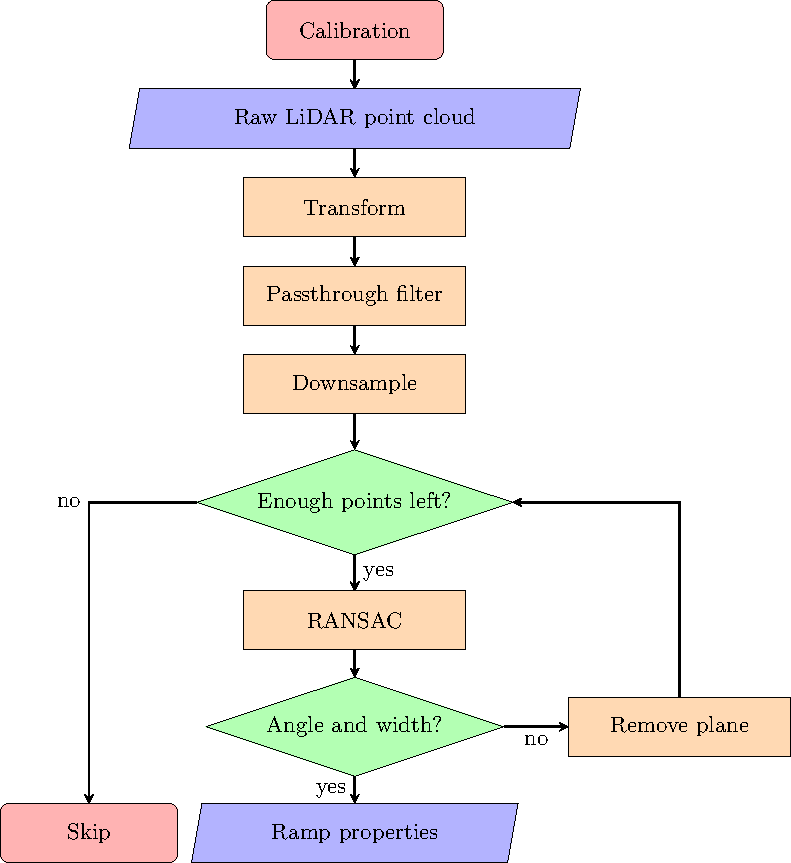
\includegraphics{Graphics/TikZ/flowchart_lidar.pdf}
	\caption[Flow chart \glsentryshort{lidar} algorithm]{Flow chart of the ramp detection algorithm using the \acrshort{lidar} sensor.}
	\label{fig:flowchart_lidar}
\end{figure}



\section{Camera based}
\label{sec:methods_camera}
In this section an approach using the images captured by the camera to detect a ramp is presented.
At first, the choice of a deep learning network as the method of choice to solve this task is explained.
In the next section the generation of the dataset used for the training is described.
The training of the network and the choice of the different hyperparameters is discussed in \cref{ssec:training}.
And in the last section it is described, how the 2D prediction of the network can be used, to extract the ramp region from a point cloud.

\subsection{Approach}
Different techniques to detect objects exist, more classic methods like edge detection and thresholding or more sophisticated methods like machine learning.
While less complex methods like edge detection and thresholding might work, they require a well lit environment with a high contrast between different textures, which is not the case in the parking garage.
Furthermore, the features need to be chosen manually, and the algorithm would most probably only work in a very limited certain environment.\\
That is why a deep learning method has been chosen instead.
It is more robust and can easily be adapted to other environments.
The choice of the network depends on the problem.
Different approaches such as object detection, instance or semantic segmentation are available.
For this project, the instance semantic approach was chosen.
While the object detection approach requires the least computational effort, it only provides a bounding box around the object.
Both segmentation approaches on the other hand create a mask around the object, allowing for a more accurate localization of the object.
For the specific task of detecting ramps in parking garages the semantic segmentation would probably be enough since most times only one ramp will be visible, in which case the semantic and instance segmentation will be the same.
But the instance segmentation approach is more general and can be adapted more easily to support also the detection of other objects.\\
That is why the mask \gls{rcnn} architecture is used in this thesis.
It allows for instance segmentation, which means that multiple objects of the same class can be detected as distinct objects.
While for this task only one class is used (ramp) and most times only one object will be visible, the network can be easily expanded to support multiple classes and is already supporting the detection of multiple ramps at once.
Furthermore, it is well documented, and different implementations are already available for use.\\
For this thesis the open-source library \texttt{Detectron2}~\footnote{\url{https://github.com/facebookresearch/detectron2}} \cite{Wu2019} developed by Facebook is chosen as the framework.
It is widely used and also provides a number of pretrained networks, which can be used for transfer learning.
Transfer learning is the process of training a new model on top of an existing one.
This provides multiple advantages over training a new model from scratch, such as a great reduction of the training time and hence also the use of resources, a better accuracy and reducing the risk of overfitting.\\
A model trained on the \gls{coco} dataset \cite{Lin2014} is used as the basis for the training of the network.
\gls{coco} is a large-scale dataset consisting of more than \num{200000} labeled images with various annotations (e.g. bounding boxes, segmentation masks, image captions) of 80 different object categories (e.g. car, chair, dog, person, train).
It is often used to benchmark neural network algorithms and to compare their performance.\\
Since no class of type ramp already exists in the \gls{coco} dataset, an own dataset has to be created.


\subsection{Dataset}
While several datasets specifically for the task of autonomous driving already exist, no dataset with ramps as a class could be found.
That is why an own dataset had to be created, by taking pictures of a ramp and labeling them by hand.
To reduce the workload, for the creation of the dataset only straight ramps of one specific parking garage are considered.
An image of the three ramps used for the training is shown in \cref{fig:img_augmentated} on the left-hand side.
Multiple recordings of each ramp were made from different distances and angles, by mounting a camera on the roof of a car and driving the car in the direction of the ramp.
The images were taken from a video with a frame rate of 30, but since the car approached the ramp with a low speed of \SI{5}{\kilo\metre\per\hour}, the difference between two frames is very small.
Since many pictures of the more or less same scenery do not provide any extra information, while increasing the training time and the potential of overfitting, only every 30th image (one every second) was used.
In the end, 144 different images of three ramps were collected.\\
Since the training of the network is based on supervised learning, the images have to be labelled manually.
For this task the tool \texttt{labelme}~\footnote{\url{https://github.com/wkentaro/labelme}} \cite{Wada2018} is used.
Each ramp is labelled using a polygon consisting of four points, placed at the corners of the ramp.
Only the drivable area of the ramp is marked, and the curbside is not considered.
The \texttt{labelme} tool creates an annotation containing the coordinate of each point and the class of the marking.
The format of the annotation had to be converted to the \gls{coco} format, to allow for the training using the \texttt{Detectron2} library.
The \gls{coco} format contains information about the segmentation mask consisting of the coordinates of the polygon, the bounding box and the class of the object.
\begin{figure}[htb]
	\centering
	\begin{subfigure}{.47\linewidth}
		\centering
		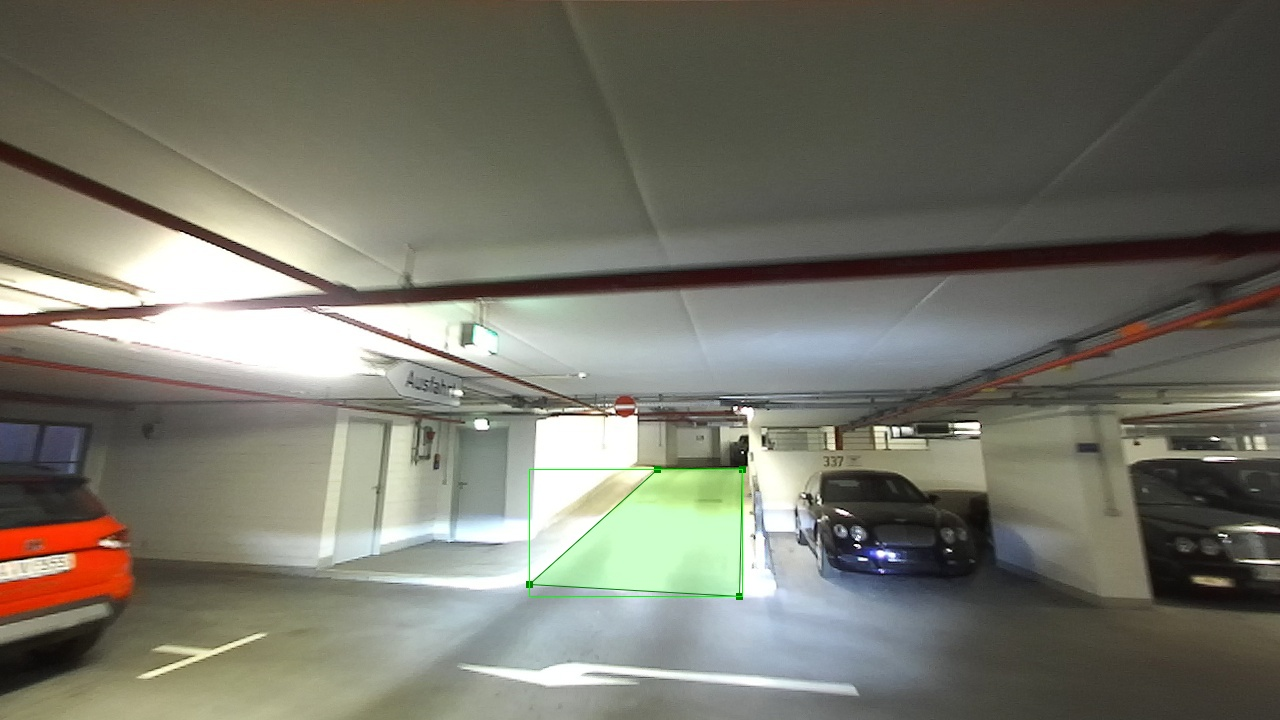
\includegraphics[width=1\linewidth]{orig.jpg}
		\caption{Original image}
	\end{subfigure}
	% \hfill
	\begin{subfigure}{.47\linewidth}
		\centering
		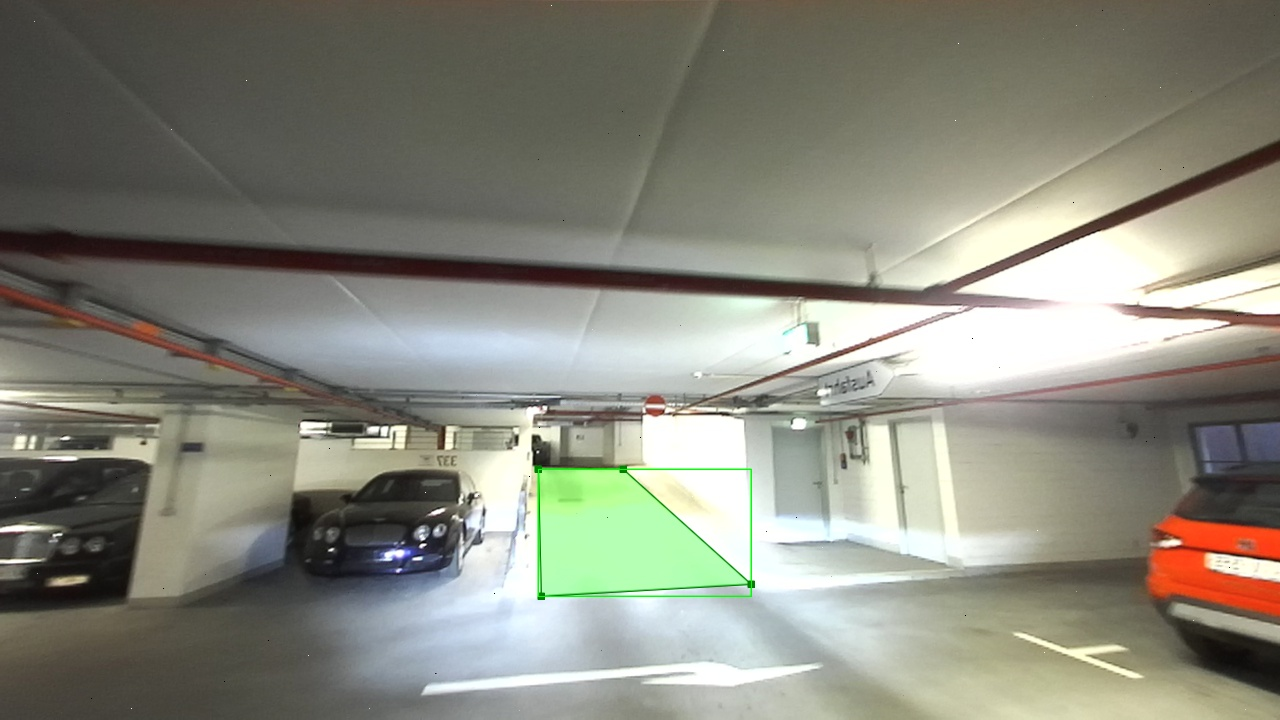
\includegraphics[width=1\linewidth]{aug.jpg}
		\caption{Augmented image}
	\end{subfigure}
	\\
	% \hfill
	\begin{subfigure}{.47\linewidth}
		\centering
		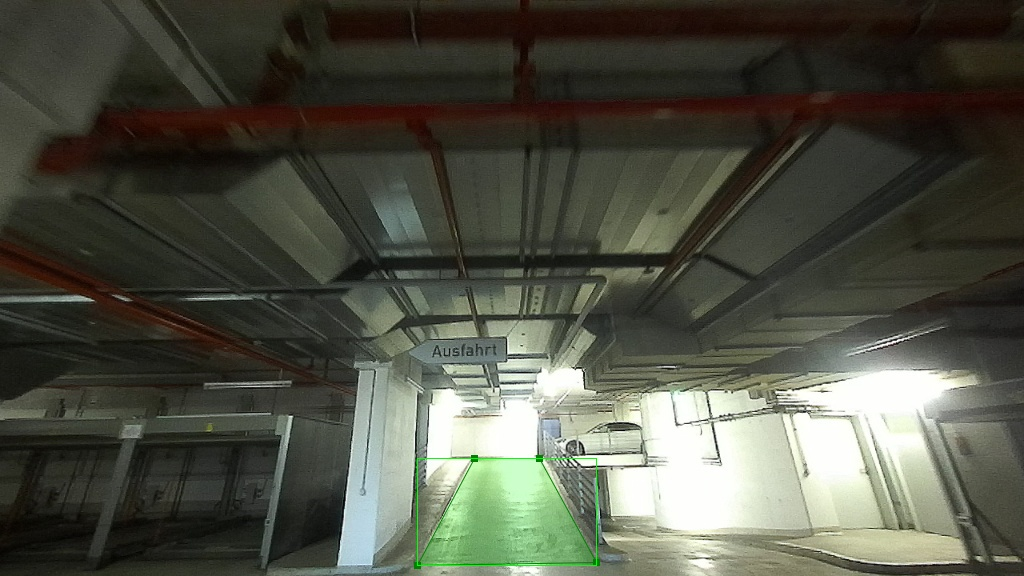
\includegraphics[width=1\linewidth]{orig2.jpg}
		\caption{Original image}
	\end{subfigure}
	\begin{subfigure}{.47\linewidth}
		\centering
		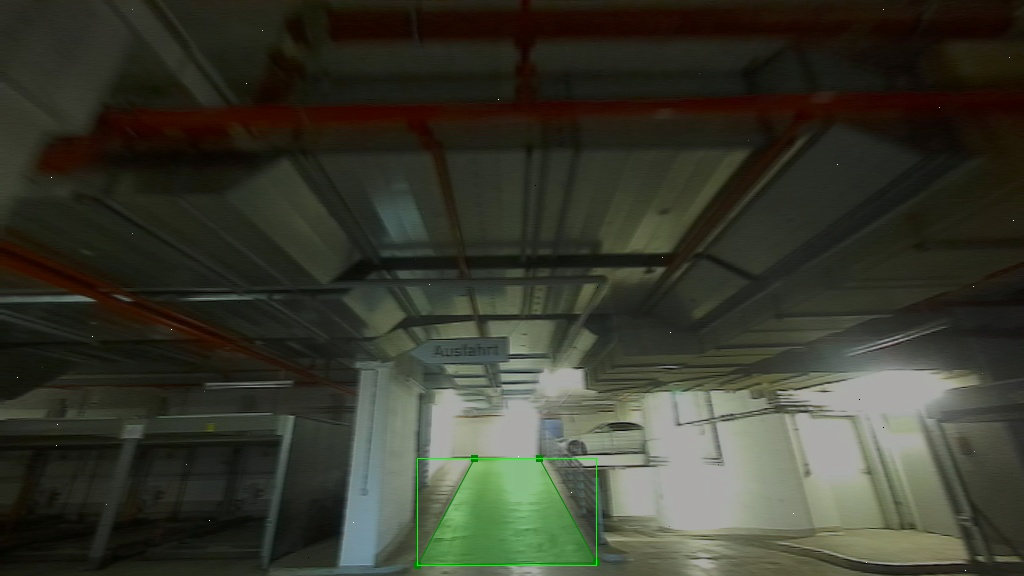
\includegraphics[width=1\linewidth]{aug2.jpg}
		\caption{Augmented image}
	\end{subfigure}
	\\
	% \hfill
	\begin{subfigure}{.47\linewidth}
		\centering
		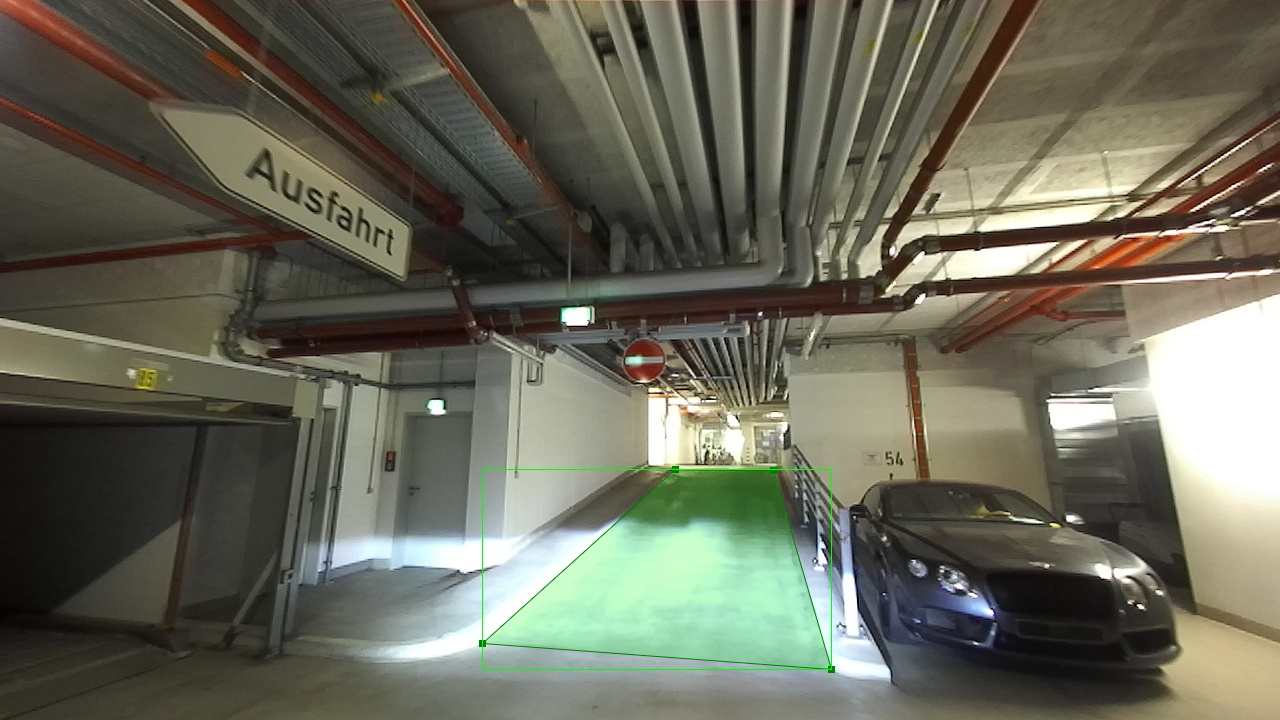
\includegraphics[width=1\linewidth]{orig3.jpg}
		\caption{Original image}
	\end{subfigure}
	\begin{subfigure}{.47\linewidth}
		\centering
		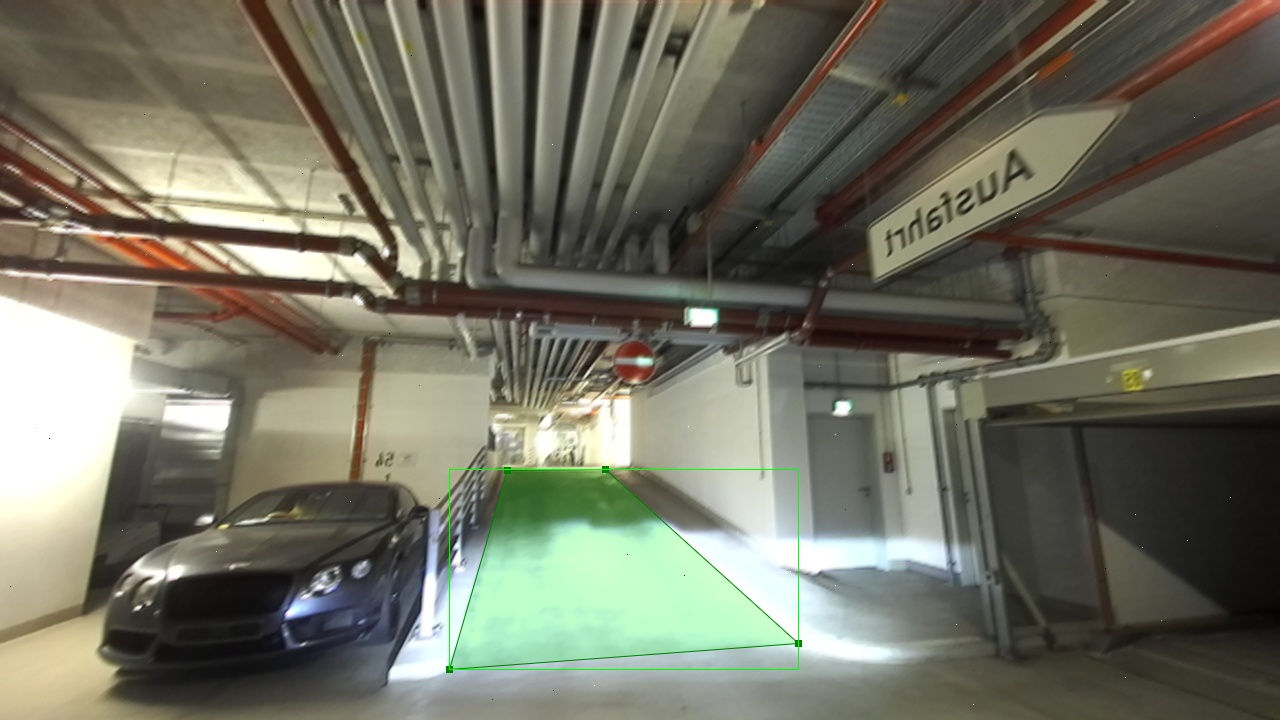
\includegraphics[width=1\linewidth]{aug3.jpg}
		\caption{Augmented image}
	\end{subfigure}
	\caption[Augmented images]{The three ramps used for the training. The augmented images are shown on the right-hand side and the manually created label is marked green.}
	\label{fig:img_augmentated}
\end{figure}


\subsection{Training}
\label{ssec:training}
Since the size of the dataset is not very great, the training of the network is challenging, because it increases the risk of overfitting.
To alleviate the problem, data augmentation is used in addition to the previously mentioned transfer learning.
Data augmentation provides a good alternative to when the collection of more data is not feasible or possible \cite{Shorten2019}.
It increases the size of the dataset by adding slightly modified versions of the original images.
Common transformations are horizontal or vertical flipping of the image, cropping, adding noise, blur or changing the brightness and contrast of the image.
The library \texttt{imgaug}~\footnote{\url{https://github.com/aleju/imgaug}} \cite{Jung2018} is used for this task.
In addition to editing the image, it automatically adapts the annotation according to the new position of the label, e.g. when flipping the image.\\
The following augmentations techniques are used to artificially increase the dataset: horizontal flipping of the image (with a probability of 50\%), changing the brightness by \SIrange{-20}{20}{\percent}, changing the contrast by \SIrange{-20}{10}{\percent}, adding motion blur with a kernel size of 3 and adding salt and pepper (turning some pixels black or white, simulating dead pixels).
Some examples of the augmented images are shown in \cref{fig:img_augmentated} on the right-hand side.
In each picture the annotation is shown as a mask and bounding box in green.
Note that the label is automatically transformed when flipping the image.
All the added changes are also common occurrences in the real world, which should help to improve the accuracy of the network in other environments.
One augmentation is performed on each image which is then added to the dataset.\\
To evaluate the performance of the network, the dataset has to be split into a training and a validation set.
The split is done before the data augmentation to ensure, that the training set does not contain any only slightly modified versions of the images used in the validation set.
Due to the small size of the dataset, 80\% of the dataset is used for the training and 20\% for the validation set.\\
The accuracy of the network depends on the correct choice of multiple hyperparameters.
Since the dataset is small and thus the training using transfer learning does not take very long, different hyperparameter configurations could be tested to find the best one.
One of the most important parameters is the learning rate.
It is often in the range of \SIrange{0.0}{1.0}{} and describes how fast the weights of the network are updated.
Is the learning rate too low, the training of the network takes a longer time and might not converge to find a solution, whereas if the learning rate is too high, a suboptimal solution might be found.
The learning rate is often initially set to a high value and then slowly reduced, which helps both optimization and generalization.
The speed of the decay of the learning rate can be based on many things, such as the number of steps in the training, the time, or it can be reduced exponentially.
% In this thesis, an approach where the learning rate is decayed after every $n$ steps is used.
Another parameter, specifically for the mask \gls{rcnn} neural network architecture, is the number of \gls{roi} proposals.
As described in \cref{sssec:rcnn}, the image is divided into a grid of \glspl{roi}.
The number of \gls{roi} proposals determines how many of those \glspl{roi} are taken into account for the calculation of the loss function.
It can be chosen lower than the size of the grid to accelerate the training.
The final parameter which will be varied is the number of epochs.
It describes how often the network is trained on the entire dataset, a higher number of epochs means a longer training time, but usually also a better performance, except if it is chosen to high, in which case it can lead to overfitting.
Because the dataset is small, has only one class and contains similar images, the number of epochs can be chosen fairly small.

\subsection{Point cloud extraction}
The ZED 2i stereo camera used in this thesis also generates a point cloud.
More information about the camera will be described in \cref{ssec:camera}.
The 3D point cloud can be projected onto the 2D camera image.
For the projection, the rotation vector and translation from the point cloud frame to the camera frame is necessary, as well as the intrinsic camera matrix $A$.
Because the ZED 2i stereo camera records both the point cloud and camera image at once, the rotation and translation between the two frames is zero.
Using the \texttt{projectPoints} function of the \texttt{opencv} library \cite{Bradski2000}, the point cloud is projected onto the camera image.
The camera image is then fed into the network, which predicts a bounding box and segmentation mask of the ramp.
Then, using the predicted bounding box or the segmentation mask, all the projected points outside the box or mask are removed.
The points are then transformed back into the 3D space.
Now that only points inside the ramp region are left, the \gls{ransac} algorithm can be applied.
It is used to find the best fitting plane of all the inliers and removes potential outliers.
Different properties of the ramp can now be calculated, as described in \cref{sssec:ramp_detecion_lidar}.\\
Instead of using the point cloud generated by the camera, the point cloud of the \gls{lidar} can be used as well.
The \gls{lidar} point cloud is more accurate, but the projection of the \gls{lidar} points onto the camera image is more difficult since the rotation and translation difference between both sensor frames is not zero anymore and must be measured by hand, which is subject to error.
\chapter{Results}
\label{ch:Results}
% Do not write long version of imu or lidar acronym again
\glslocalunset{imu}
\glslocalunset{lidar}
In this chapter the results of the different proposed methods will be presented.
At first, the collection of the reference data will be explained.
The different metrics used for the evaluation of the results will be described in \cref{sec:performance_measures}.
The different methods using the \gls{imu} are analyzed in \cref{sec:eval_imu}.
Afterwards the performance of the \gls{lidar} algorithm will be discussed in \cref{sec:eval_lidar} and finally the results of the object detection using the camera will be presented in \cref{sec:eval_camera}.


\section{Evaluation Concept}
During each test drive the measurements of the accelerometer and gyroscope of the \gls{imu} (of both \glspl{imu}, myAHRS+ and of the \gls{imu} integrated in the ZED 2i camera), the camera image of the ZED 2i camera and the point cloud generated by the \gls{lidar} are recorded.
Only one \gls{lidar} could be mounted at a time, so the Velodyne UltraPuck was used for most test drives, but two recordings were also made using the Robosense.
Furthermore, the wheel speeds were recorded when available, which was only the case when driving a ramp down or only half-way up, as mentioned in \cref{sec:car}.\par
To prevent an overfitting of the model it is important to have different test scenarios.
As mentioned in \cref{sec:garage}, four different ramps were available to test the model.
For the evaluation of the \gls{imu} only the ramps A B, and D will be used.
Multiple test drives were made for each scenario, the most drives where performed on ramp A.
Because the wheel speed sensor measurements are needed for some methods, which are only available in a special mode where the power of the car is very limited, the ramps A and B could only be driven halfway up.
But a full recording including the wheel speed measurements could be done for ramp D and A, when driving down.\par
The algorithms using the \gls{lidar} and camera only detect ramps going up, so only the ramps A, B and C were used.
Furthermore, a test drive without any ramps in sight was made to test if false positives are being detected.



\section{Reference Data}
To evaluate the performance of the different algorithms a reference is necessary.
The open-source \gls{ros} package \texttt{hdl\_graph\_slam}~\footnote{\url{https://github.com/koide3/hdl_graph_slam}}~\cite{Koide2019} is used for this task.
It is based on 3D graph \gls{slam} and uses the \gls{lidar} data to map the environment and estimate the pose (position and orientation) of the car.
It uses \gls{ndt} scan matching-based odometry estimation with loop detection.
The point cloud of common features at time $t$ is compared to the point cloud from the time $t-1$ and matched against each other.
The algorithm then estimates the translation and orientation difference between those two point clouds.
In ref.~\cite{Akpnar2021} the accuracy of the HDL Graph \gls{slam} was tested and a mean error of \SI{4}{\cm} and a standard deviation of \SI{5}{\cm} was measured for an indoor scenario.\par
From the pose information of the HDL Graph \gls{slam} the pitch angle of the car can be calculated and be used as a reference for the road grade, to evaluate the performance of the different \gls{imu}-based methods.
Because the \gls{lidar} only records at \SI{10}{\hertz} and thus the estimation of the HDL Graph \gls{slam} also only updates at a rate of \SI{10}{\hertz}, but the other sensors record from \SIrange{100}{400}{\hertz}, the estimate was upsampled using a Fourier method.
Beside estimating the road grade, the \gls{imu} is used to estimate the angle and length of the ramp.
The reference value for the length can be extracted from the generated point cloud map, by measuring the distance between the corresponding points.
Because the ramp angle is not constant, the average angle of the ramp is used as reference.
The average angle \gls{ramp_ang} is calculated by measuring the length and height of the ramp and using the law of sines
\begin{equation}
    \gls{ramp_ang} = \arcsin\left(\frac{h_\mathrm{ramp}}{l_\mathrm{ramp}}\right).
\end{equation}
The \gls{lidar} is used to detect and track the distance to the ramp and also to estimate the angle, width and length.
For the evaluation of the tracking accuracy, the generated map and pose provided by the HDL Graph \gls{slam} is used again.
In the generated point cloud map, the ramp region was marked manually by visual inspection.
Then, using the position of the car, provided by the \gls{slam}, the true distance to the beginning of the ramp could be calculated, by measuring the distance of the current position to the beginning of the ramp for each frame.\par
An example of the point cloud map generated by the \texttt{hdl\_graph\_slam} package is shown in \cref{fig:pcd_plotly}.
The color of the points gives information about the z-value (height information) of the points.
The ramp region is marked by the greater points in rainbow color and the black squares visualize the trajectory of the car.
In this example the car was driven only half-way up the ramp.
As mentioned in \cref{sec:methods_camera}, the camera is also used to identify the ramp.
Because manual labeling of all the images was necessary for the training of the network, the labels can be used as a reference.
\begin{figure}[htb]
    \centering
    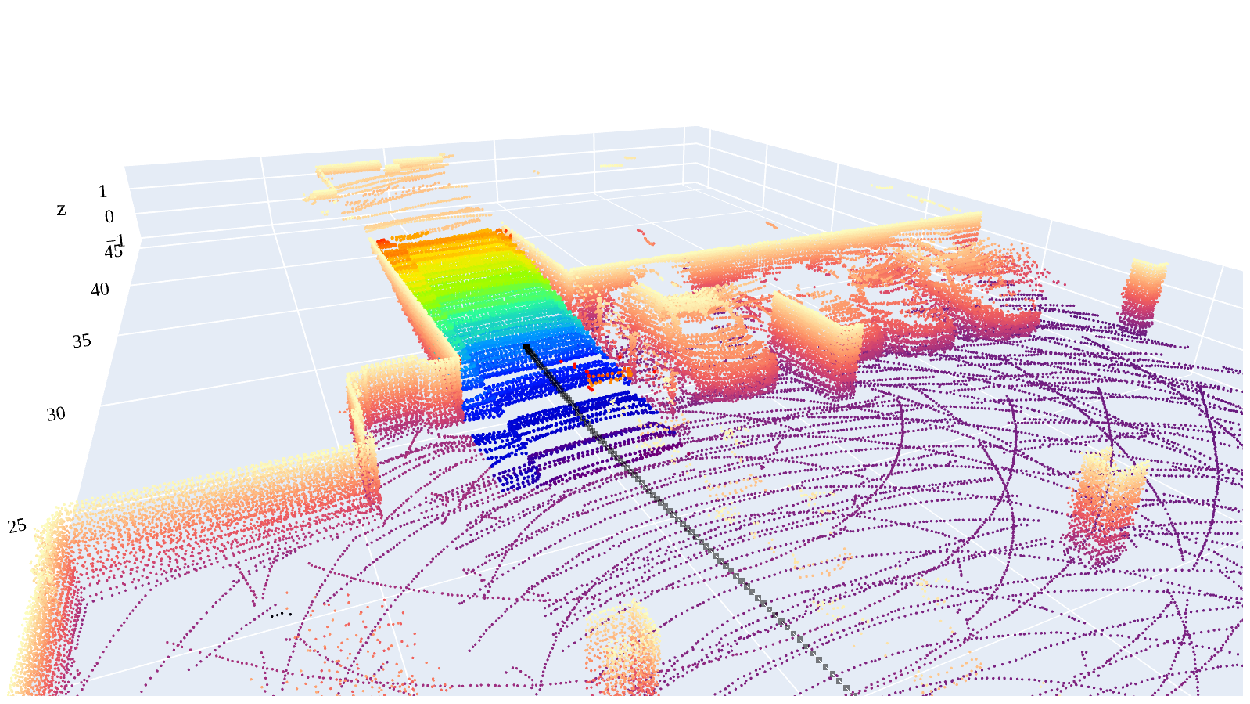
\includegraphics[width=1\linewidth, trim={0 0 0 2cm}, clip]{pcd_plotly}
    \caption[Generated point cloud map]{The by the \texttt{hdl\_graph\_slam} package generated point cloud map. The ramp region was selected manually by visual inspection and is marked by the rainbow-colored points. The black squares visualize the trajectory of the car.}
    \label{fig:pcd_plotly}
\end{figure}



\section{Performance Measures}
\label{sec:performance_measures}
Using the \gls{imu}, the pitch angle of the car is estimated over time.
The goodness of the fit between the estimation $\hat{y} = (\hat{y}_i, \dots, \hat{y}_n)^\intercal$ and the reference $y = (y_i, \dots, y_n)^\intercal$ can then be described by the \gls{rmse}
\begin{equation}
    RMSE = \sqrt{\frac{1}{n}\sum_{i = 1}^n(\hat{y}_i - y_i)^2},
\end{equation}
which quantifies how much the predicted values differ from the reference value on average.
It is defined in the range $[0, \infty)$, with a value of 0 indicating a perfect fit.\par
The same can be applied to the estimation for the angle, width, length and distance to the ramp by the \gls{lidar}-based method.
The only difference is that the reference angle, width and length are constant and thus the \gls{rmse} is basically the same as the standard deviation in this case.
Furthermore, the coefficient of determination $R^2$ is used to evaluate the pitch angle estimation
\begin{equation}
    R^2 = 1 - \frac{\sum\limits_{i = 1}^n(\hat{y}_i - y_i)^2}{\sum\limits_{i = 1}^n(\hat{y}_i - \overline{y})^2},
\end{equation}
where $\overline{y}$ indicates the mean of the reference.
The goodness of the fit is described in the range from 0 to 1, where 1 describes a perfect fit.\par
The \gls{lidar} is used to detect a ramp, and to calculate its properties if a ramp is detected.
The detection rate is evaluated by using the number of \glspl{tp} and \glspl{fn}.
What is counted as \gls{tp} or \gls{fn} always depends on the use case.
In the \gls{lidar} scenario, a frame is labeled as \gls{tp} if the ramp is visible to the \gls{lidar}, the algorithm detected a ramp and at least 70\% of the detected points actually lie inside the ramp region.
Analogously, a frame is classified as \gls{fn}, if a ramp is visible but less than 70\% of the detected points lie inside the ramp region.
Furthermore, when a ramp was detected even though none was visible, the frame is labeled as \gls{fp}.\par
The performance of the neural network can be evaluated in several ways.
One commonly used metric in the field of computer vision is the \gls{ap}.
It is a detection evaluation metric, commonly used by the \gls{coco} dataset.
It is based on the precision and recall score, which can be calculated by
\begin{equation}
    \text{Precision} = \frac{TP}{TP+FP}
\end{equation}
\begin{equation}
    \text{Recall} = \frac{TP}{TP+FN}.
\end{equation}
The precision gives information about how accurate the predictions are and the recall gives information about how much of the ground truth is detected.
The area under the precision-recall curve is the \gls{ap} score.
So, unlike the name might suggest, the \gls{ap} score is not actually just the average of the precision score.
Otherwise, a model which correctly detects some objects in the image, but misses others, would still achieve a score of 1.
Similarly to the \gls{lidar}, it first must be defined what classifies as a \gls{tp} and a \gls{fp}.
For this, a new metric is introduced, the \gls{iou}, which is defined as
\begin{equation}
    \text{\acrshort{iou}} = \frac{\text{Area of Overlap}}{\text{Area of Union}}.
\end{equation}
The area of overlap is defined as the intersection between the predicted and ground truth bounding box, and the area of union is the area of both boxes added together.
Instead of a bounding box, a segmentation mask can be used as well.
A perfect detection would have an \gls{iou} score of 1.
Because an \gls{iou} score of 1 is nearly impossible, a frame is labeled as \gls{tp} instead, if the \gls{iou} score is greater than a certain threshold $m$.
The score is then written as $\text{AP}_{m}$.
For example, $\text{AP}_{50}$ means how many detections have been made with an \gls{iou} score of at least 50\%.
Since selecting a meaningful threshold for the \gls{ap} score depends on the dataset, the \gls{map} is often used instead.
The \gls{map} score is the average over multiple \gls{iou} thresholds for all the different classes.
It is calculated by averaging all \gls{ap} scores in the range of 50\% to 95\% with a step size of 5\%, meaning that the average of 10 different values is used.
\section{\glsentryshort{imu}}
\label{sec:eval_imu}
In this section the different methods to estimate the road grade using the \gls{imu} are being evaluated.
The results for two different drives are visualized.
Lastly, the estimated average ramp angle and length are being compared to the ground truth.

\subsection{Road Grade Estimation}
The ramp detection using the \gls{imu} relies on the correct estimation of the road grade angle.
Hence, the evaluation of the goodness of the estimation is necessary to determine the performance of the ramp detection algorithm.\par
Different recordings of different ramps were made, but the results will be discussed on only two test drives.
Furthermore, two different \glspl{imu} were used, but only the measurements of one \gls{imu} will be used to present the results, since both produced similar results.
Because the \gls{imu} of the ZED camera is slightly more accurate as shown in \cref{tab:imu_datasheets}, only those measurements will be used.\par
In the first drive the car was accelerated from stand still and drove up ramp A about half-way up.
As explained in \cref{sec:car}, the ramp could not be driven completely, due to the need of the odometer readings, which are only available when the motor output is limited.
The result of using only the raw measurements of the \gls{imu} for the pitch angle calculation is illustrated in \cref{fig:imu_raw_angle}.
\begin{figure}[htb]
    \centering
    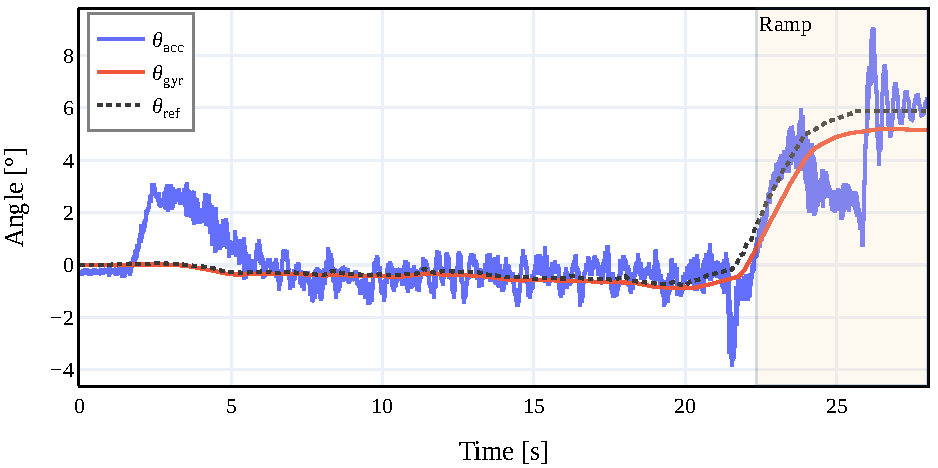
\includegraphics[width=.9\linewidth]{imu_raw_angle.pdf}
    \caption[Angle estimation using raw measurements]{Pitch angle estimation from the raw accelerometer and gyroscope measurements. The drive did start from stand still and did end in the middle of the ramp.}
    \label{fig:imu_raw_angle}
\end{figure}
The measurement by the accelerometer is very noisy and is easily influenced by accelerations other than gravity, which can be seen at time \SIrange{2}{4}{\second}, where the car started driving.
The gyroscope on the other hand provides good short-term accuracy and is not influenced by other accelerations, but is slowly drifting over time.
The reference is taken from the orientation estimation of the \texttt{hdl\_graph\_slam} package, which uses the \gls{lidar} data.
The time frame during which the car was on the ramp is marked by the yellow coloring.
The beginning of the ramp is classified as the point, where the reference data surpasses \ang{1.5}.\par
The gravity method tries to overcome the problem of the accelerometer of also detecting other accelerations than gravity, by subtracting the car's acceleration from the accelerometer measurement.
The car's acceleration $\vb{a}_\mathrm{odom,x} $ was calculated by calculating the derivate of the low-pass filtered car velocity $v_\mathrm{car} $, which was calculated from the wheel speed measurements.
\Cref{fig:imu_odometer_acc} shows the (low-pass filtered) acceleration measured by the \gls{imu} along the x-axis and the (low-pass filtered) car's acceleration.
\begin{figure}[htb]
    \centering
    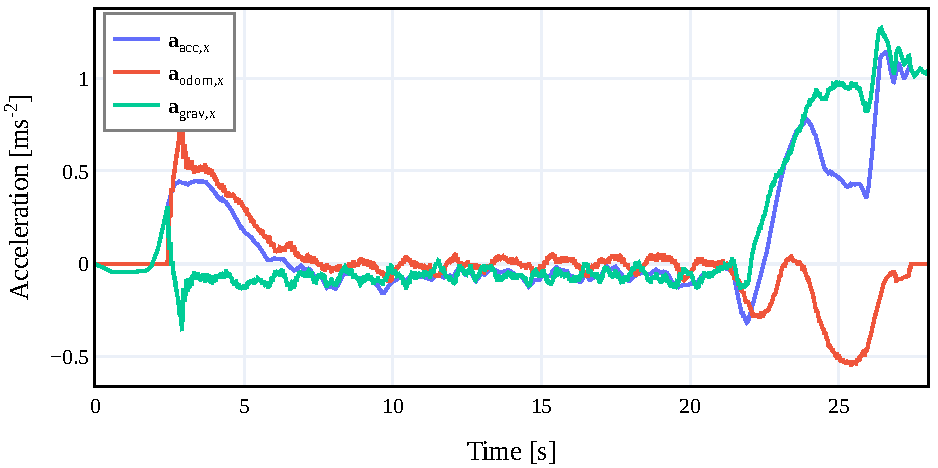
\includegraphics[width=.9\linewidth]{imu_odometer_acc.pdf}
    \caption[Measured acceleration from \glsentryshort{imu} and odometer]{The measured acceleration in x-direction by the \glsentryshort{imu} and the acceleration derived from the wheel speed measurements and the difference between both.}
    \label{fig:imu_odometer_acc}
\end{figure}
And $\vb{a}_\mathrm{grav,x} $ is the acceleration measured by the \gls{imu} from which the car acceleration $\vb{a}_\mathrm{odom,x} $ was subtracted.
It can be seen, that especially at the beginning of the ramp (\SIrange{21}{23}{\second}) the gravity method shows it advantages.
The deceleration before entering the ramp is measured by both sensors and thus cancels out each other.
The same can be seen in the initial acceleration phase, where the car starts to drive from still stand (\SIrange[]{2}{4}{\second}).
Although both sensor are synchronized in time, the \gls{imu} senses the acceleration earlier than the wheel speed sensors which leads to a slight pike.
This could be due to the wheel speed sensors having a certain velocity threshold, below which they do not pick up any changes.
Other reasons for the difference could be, that other forces than the one from the car are present, e.g. from the suspension of the car, vibrations due to the road quality or movement in the car, which are not measured by the wheel speed sensors.
Moreover, the approximations made by calculating the finite difference of the car velocity to get the car acceleration have a negative influence on the result.\par
The resulting angles calculated from the accelerations can be seen in \cref{fig:imu_odometer_angle}.
\begin{figure}[htb]
    \centering
    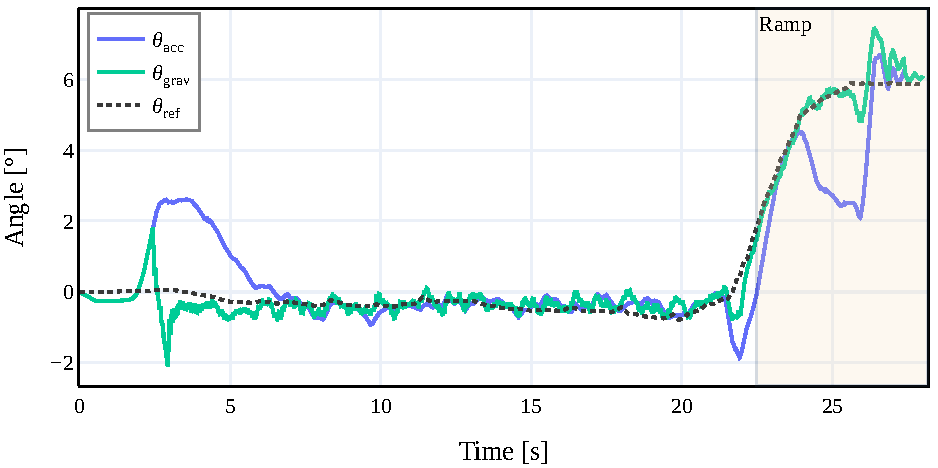
\includegraphics[width=.9\linewidth]{imu_odometer_angle.pdf}
    \caption[Angle estimation using the gravity method]{Pitch angle estimation using only the accelerometer compared to the gravity method, which additionally uses the wheel speed measurements.}
    \label{fig:imu_odometer_angle}
\end{figure}
It can be seen that the gravity method improves the estimation accuracy, compared to when only the accelerometer data is used.
Especially the angle at the start and on the ramp is more accurately described when subtracting the odometer data from the accelerometer data for the calculation.
But it can also be seen that the time synchronization between both signals is important, which becomes apparent during the initial acceleration phase.
Here, the subtraction leads to a negative value, which neither sensor had measured.\par
Another way to improve the estimation is using a complementary filter.
The results of which, together with all other methods, are shown in \cref{fig:imu_all_angles}.
Those are the results of a new drive, where the car was driven the ramp D and afterwards ramp A down.
\begin{figure}[htb]
    \centering
    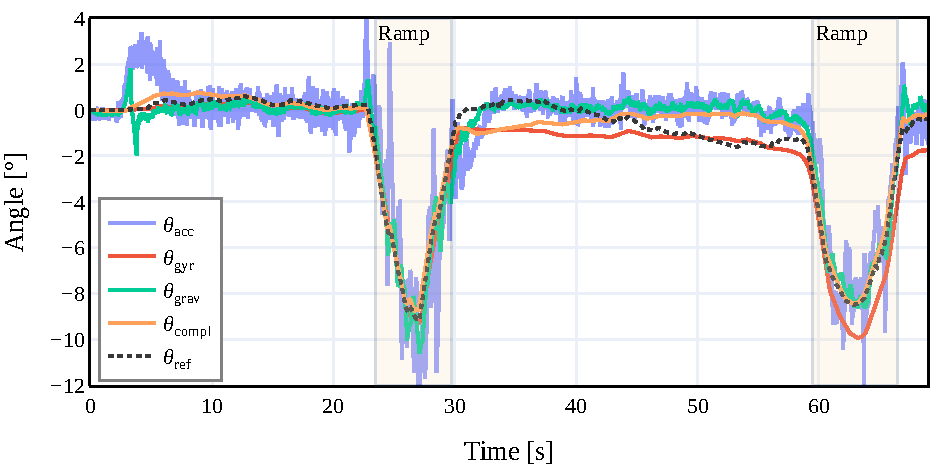
\includegraphics[width=.9\linewidth]{imu_all_angles.pdf}
    \caption[Angle estimation comparison of all methods]{Comparison of different methods to estimate the pitch angle. Two different ramps were driven down successively.}
    \label{fig:imu_all_angles}
\end{figure}
The complementary filter uses the estimation of the gyroscope measurements and corrects them using the accelerometer measurements to prevent drift.
It can be seen that the estimation using the complementary filter closely follows the reference except for the part between the two ramps (\SIrange{30}{60}{\second}).
Also, it has no offset at the end, unlike the estimation from the gyroscope data.
The results of the other methods applied to the recordings of the same ride are also shown in the same figure.
Using the gyroscope measurements, the angle estimation follows the reference data very closely for the first ramp.
But at the end a drift can be observed.
The gravity method reduces the spikes of the raw accelerometer estimation, but introduces a new error at the beginning, due to the odometer readings being slightly shifted in time in regard to the accelerometer readings.\par
While a visual inspection gives a first impression on which method performs the best, the use of different metrics allows for a more accurate evaluation.
The \gls{rmse}, $R^2$ as well as the maximal error of the different methods when driving up, for two kinds of ramps, are shown in \cref{tab:eval_imu_up}.
Multiple recordings have been made for each ramp, but in all of them the car started from stand still and ended in the middle of the ramp.
The average of all drives was then calculated.\par
The estimation using the raw accelerometer data performs the worst and has the greatest maximal error.
Using the gyroscope the deviation from the reference data is fairly small, which can be seen in the maximal error.
But due to the drifting the errors cumulate, resulting in a high \gls{rmse} value.
The acceleration method performs well, but is negatively influenced by the acceleration from stand still, during which the accelerometer and wheel speed data are not properly aligned.
The best results are achieved using the complementary filter.
\begin{table}[htb]
    \centering
    \caption[Road grade estimation for uphill drives]{Road grade estimation when driving ramps up, using different methods.}
    \label{tab:eval_imu_up}
    \resizebox{\textwidth}{!}{
        \begin{tabular}{lcccccc}
            \toprule
                                & \multicolumn{3}{c}{\textbf{Ramp A}} & \multicolumn{3}{c}{\textbf{Ramp B}}                                                                                                                                   \\
            \midrule
            \textbf{Method}     & \textbf{RMSE} [\si{\degree}]        & $\mathbf{R^2}$                      & $\mathbf{Error_{max}}$ [\si{\degree}] & \textbf{RMSE} [\si{\degree}] & $\mathbf{R^2}$   & $\mathbf{Error_{max}}$ [\si{\degree}] \\
            \cmidrule(lr){2-4}   \cmidrule(lr){5-7}
            Accelerometer       & 0.875                               & 0.675                               & 4.944                                 & 0.650                        & 0.787            & 3.378                                 \\
            Gyroscope           & 0.508                               & 0.905                               & 1.373                                 & 0.768                        & 0.802            & $\mathbf{1.594  }$                    \\
            Acceleration method & 0.357                               & 0.954                               & 2.482                                 & 0.351                        & $\mathbf{0.955}$ & 1.707                                 \\
            Complementary       & $\mathbf{0.273} $                   & $\mathbf{0.976}$                    & $\mathbf{1.231 }$                     & $\mathbf{0.324}$             & 0.952            & 1.647                                 \\
            % Complementary grav  & 0.371                               & 0.948                               & 1.990                  & 0.358            & 0.951            & 1.211                  \\
            \bottomrule
        \end{tabular}
    }
\end{table}
In \cref{tab:eval_imu_down} the average results for down drives are shown.
The data are from a test drive in which at first the ramp C was driven down, followed by ramp A in one consecutive drive.
The drive was performed multiple times and the average of all results was calculated again.
The estimations for one exemplary ride were illustrated in \cref{fig:imu_all_angles}.
The values for ramp C correspond to the measurements from \SIrange{0}{31}{\second} and the measurements from \SI{31}{\second} until the end are attributed to ramp A.
It can be seen that at the beginning (ramp C) the gyroscope performs the best, but with increasing time the drift negatively impacts the results.
All methods perform significantly worse in the second part of the drive (ramp A), due to the deviation of the reference value in the time frame between the two ramps.
But when looking at the graph in \cref{fig:imu_all_angles} it can be seen, that the gravity method and especially the complementary filter closely follows the reference data.
\begin{table}[htb]
    \centering
    \caption[Road grade estimation for downhill drives]{Road grade estimation when driving ramps down, using different methods.}
    \label{tab:eval_imu_down}
    \resizebox{\textwidth}{!}{
        \begin{tabular}{lcccccc}
            \toprule
            \textbf{Method}     & \multicolumn{3}{c}{\textbf{Ramp C}} & \multicolumn{3}{c}{\textbf{Ramp A}}                                                                                                                                   \\
            \midrule
                                & \textbf{RMSE} [\si{\degree}]        & $\mathbf{R^2}$                      & $\mathbf{Error_{max}}$ [\si{\degree}] & \textbf{RMSE} [\si{\degree}] & $\mathbf{R^2}$   & $\mathbf{Error_{max}}$ [\si{\degree}] \\
            \cmidrule(lr){2-4}   \cmidrule(lr){5-7}
            Accelerometer       & 0.894                               & 0.746                               & 8.291                                 & 0.938                        & 0.784            & 3.967                                 \\
            Gyroscope           & $\mathbf{0.219}$                    & $\mathbf{0.990}$                    & $\mathbf{0.736}$                      & 0.784                        & 0.867            & $\mathbf{1.481}$                      \\
            Acceleration method & 0.369                               & 0.964                               & 2.211                                 & $\mathbf{0.719}$             & $\mathbf{0.872}$ & 2.136                                 \\
            Complementary       & 0.327                               & 0.977                               & 1.184                                 & 0.753                        & 0.862            & 2.131                                 \\
            \bottomrule
        \end{tabular}
    }
\end{table}


\subsection{Ramp Properties Estimation}
Now that the estimation of the road grade is done, the ramp properties can be estimated.
The estimated ramp angles and the corresponding deviation from the reference value for three different ramps are listed in \cref{tab:eval_imu_angle}.
All the different methods seem to underestimate the angle when driving up (ramp A and B) or overestimate it when driving down (ramp D).
Because ramp A and B could only be driven half-way up, it could be possible that the average angle had not been reached yet.
Overall it can be seen that the complementary filter and the acceleration method perform the best.\par
\begin{table}[htb]
    \centering
    \caption{Estimation of ramp angle.}
    \label{tab:eval_imu_angle}
    \resizebox{\textwidth}{!}{
        \begin{tabular}{lcccccc}
            \toprule
                                & \multicolumn{2}{c}{\textbf{Ramp A}} & \multicolumn{2}{c}{\textbf{Ramp B}} & \multicolumn{2}{c}{\textbf{Ramp D}}                                                                                                 \\
            \midrule
            \textbf{Method}     & \textbf{Angle} [\si{\degree}]       & \textbf{Error} [\si{\degree}]       & \textbf{Angle} [\si{\degree}]       & \textbf{Error} [\si{\degree}] & \textbf{Angle} [\si{\degree}] & \textbf{Error} [\si{\degree}] \\
            \cmidrule(lr){2-3}  \cmidrule(lr){4-5}   \cmidrule(lr){6-7}
            Accelerometer       & 4.14                                & 3.06                                & 4.75                                & 1.75                          & -10.41                        & 2.11                          \\
            Gyroscope           & 4.97                                & 2.23                                & 4.30                                & 2.20                          & -9.11                         & 0.81                          \\
            Acceleration method & 6.15                                & 1.05                                & 6.18                                & 0.32                          & -9.52                         & 1.22                          \\
            Complementary       & 5.42                                & 1.78                                & 6.12                                & 0.38                          & -9.01                         & 0.71                          \\
            \bottomrule
        \end{tabular}
    }
\end{table}
As discussed in \cref{ssec:ramp_detection_imu}, the length of the ramp can be estimated by integrating the velocity of the car over the time interval between the start and end of the ramp.
The velocity can be estimated in two different ways.
Either by using the wheel speed measurements, or by integrating the accelerometer measurements.
For the evaluation of the accuracy of the estimation, recordings of a drive with a full traverse of a ramp is necessary.
As mentioned in \cref{sec:car}, this is only possible when driving down.
Ramp D is used for this evaluation, the first part of the drive show in \cref{fig:imu_all_angles}.\\
In \cref{fig:imu_distance_velocity} different methods to estimate the velocity of the car are shown.
\begin{figure}[htb]
    \centering
    \begin{subfigure}{1\textwidth}
        \centering
        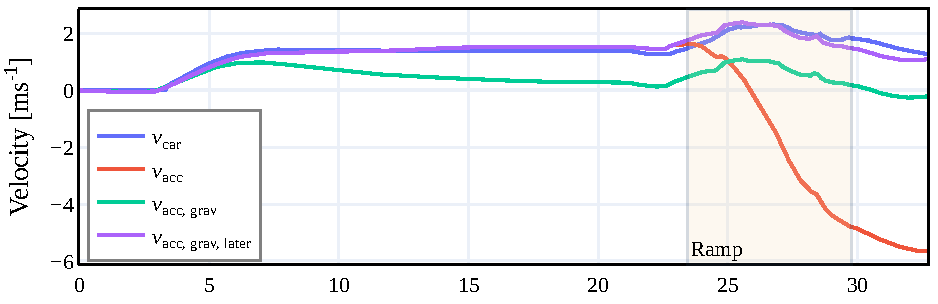
\includegraphics[width=.9\linewidth]{imu_distance_velocity.pdf}
        \caption[Car velocity estimation]{Estimated car velocity calculated from the wheel speed measurements and different methods using the accelerometer data.}
        \label{fig:imu_distance_velocity}
    \end{subfigure}
    
    % \bigskip
    \begin{subfigure}{1\textwidth}
        \centering
        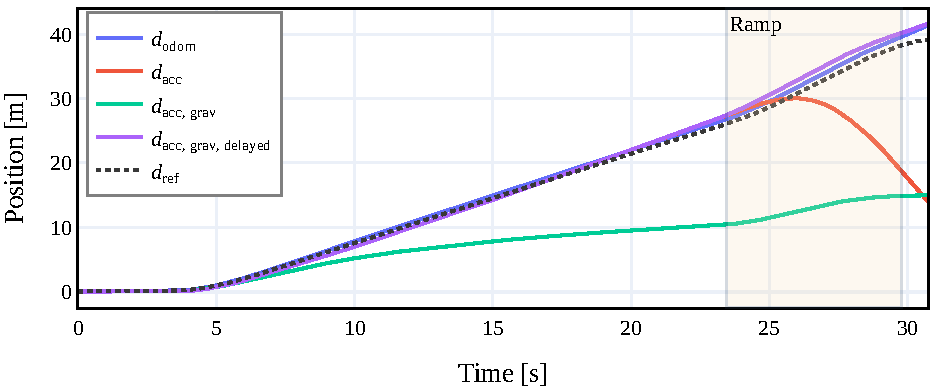
\includegraphics[width=.9\linewidth]{imu_distance_position.pdf}
        \caption[Car travelled distance estimation]{The integration of the velocity leads to the travelled distance. The length of the ramp can then be calculated from the difference between the position at the end and start of the ramp.}
        \label{fig:imu_distance_position}
    \end{subfigure}
    \caption[Ramp length estimation using various methods]{Comparison of different methods to estimate the length of the ramp.}
\end{figure}
$v_\mathrm{odom}$ is the velocity calculated from the wheel speed measurements using \cref{eq:v_car}.
The other three methods are based on the integration of the accelerometer measurements.
$v_\mathrm{acc}$ is the result of integrating the raw accelerometer measurements $\vb{a}_x$.
Because the raw signal also contains the gravity component, the estimation is not correct anymore when entering the ramp.
Up until the point where the car enters the ramp both estimations are very similar, but during the phase on the ramp the acceleration due to gravity disturbs the estimation.
This problem is partially solved by $v_\mathrm{acc, grav}$, which eliminates the gravity component by subtracting it using the pitch angle of the car, according to \cref{eq:acc_from_imu_wo_grav}.
Different angles can be used in the equation, the angle estimation using the complementary filter was chosen, since it achieved the best results.
Nonetheless, because the angle estimation of the angle is not correct at the start of the acceleration (\SIrange{3}{5}{\second}), an error is introduced.
As it can be seen in \cref{fig:imu_all_angles} the angle is slightly overestimated by the complementary filter during the acceleration phase.
This leads according to \cref{eq:acc_from_imu_wo_grav} to an underestimation of the acceleration, and thus also an underestimation of the velocity.
Due to the integration the error is cumulated over time and increases with the time.\par
This error can be fixed by introducing a new method, which ignores the angle estimation during the acceleration phase and instead assumes an angle of zero during this phase.
The result is visualized by $v_\mathrm{acc, grav, delayed}$.
For the sake of consistency, the reference data is once again calculated from the pose provided by the \texttt{hdl\_graph\_slam} package.
But it must be noted, that the data from the wheel sensors is most likely more accurate, but the results will still be compared to the reference data.\par
The estimation of the travelled distance for the different methods is shown in \cref{fig:imu_distance_position}.
Since the distance is calculated by integrating the velocity, an error is cumulated over time.
This can be seen in both $d_\mathrm{acc}$ and $d_\mathrm{acc, grav}$.
The only usable results are produced by the method using the odometer measurements and by $v_\mathrm{acc, grav, delayed}$.\par
The actual length of the ramp is calculated by subtracting the position of the car at the end of the ramp from the position at the start of the ramp.
The calculated length for the different methods and the corresponding error are shown in \cref{tab:ramp_length}.
\begin{table}[htb]
    \centering
    \caption[Ramp length estimation]{The estimation of the ramp length using different methods.}
    \label{tab:ramp_length}
    \begin{tabular}{lSS}
        \toprule
        \textbf{Method}                & {\textbf{Length} [\si{\metre}]} & {\textbf{Error} [\si{\metre}]} \\
        \midrule
        $d_\mathrm{odom} $             & 11.88                           & 0.63                           \\
        $d_\mathrm{acc} $              & -8.44                           & 20.69                          \\
        $d_\mathrm{acc, grav, } $      & 4.52                            & 7.73                           \\
        $d_\mathrm{acc, grav, later} $ & 11.85                           & 0.60                           \\
        $d_\mathrm{ref} $              & 11.25                           & 0                              \\
        \bottomrule
    \end{tabular}
\end{table}



\section{Ramp Detection (\glsentryshort{lidar})}
\label{sec:eval_lidar}
The \gls{lidar} is used to detect if a ramp is visible, track the position to the ramp as well as to estimate the angle, width and length of the ramp.
Due to the setup it was only possible to mount one \gls{lidar} at a time.
To get the best possible results the \gls{lidar} with the best resolution, especially in vertical direction, should be used.
A comparison of the resolution of the two \glspl{lidar} can be seen in \cref{fig:lidar_resolution_eval}.
\begin{figure}[htb]
    \centering
    \begin{subfigure}{1\textwidth}
        \centering
        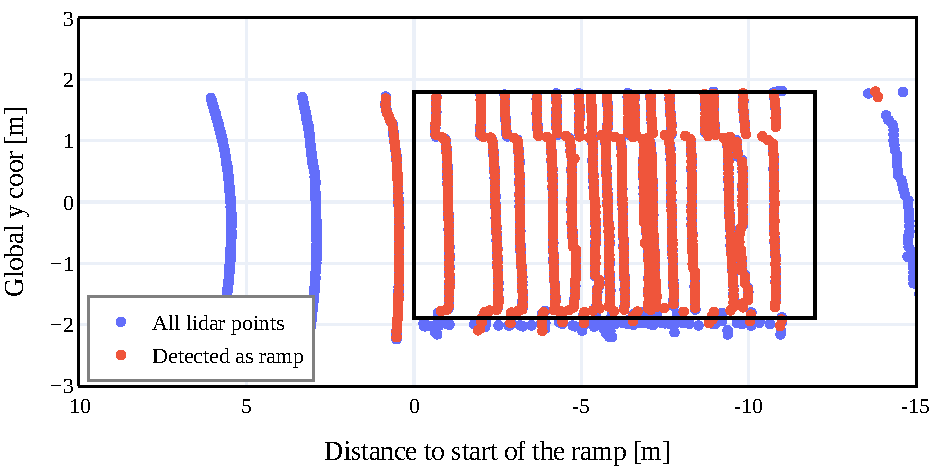
\includegraphics[width=.9\linewidth]{lidar_resolution_velodyne_eval.pdf}
        \caption{Velodyne}
        \label{fig:lidar_resolution_velodyne_eval}
    \end{subfigure}
    
    \begin{subfigure}{1\textwidth}
        \centering
        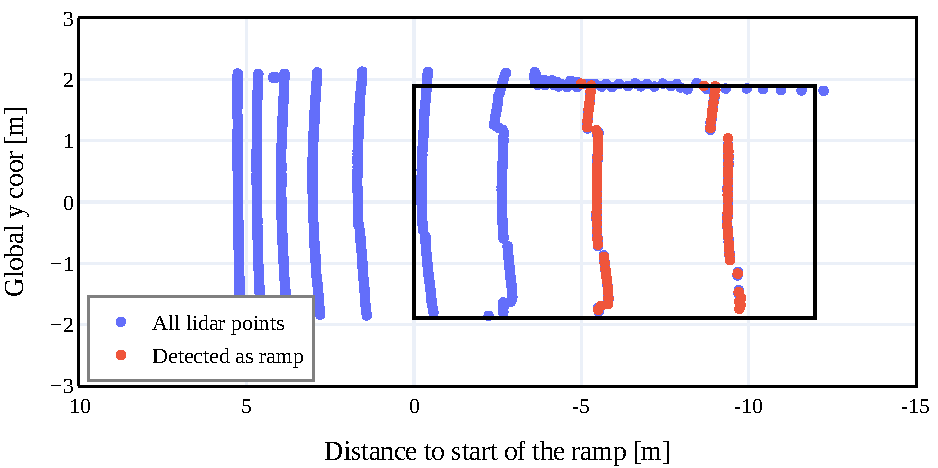
\includegraphics[width=.9\linewidth]{lidar_resolution_robos_eval.pdf}
        \caption{Robosense}
        \label{fig:lidar_resolution_robos_eval}
    \end{subfigure}
    \caption[Resolution comparison of the two \glsentryplural{lidar}]{Resolution comparison of the two \glsentryplural{lidar}. The ramp region is framed in black.}
    \label{fig:lidar_resolution_eval}
\end{figure}
Here, a top-down view on the ramp of the points measured by the \gls{lidar} at a distance of \SI{7}{\metre} to the ramp is shown.
The blue points visualize all the points which were visible to the ramp detection algorithm after the downsampling and pass through filter has been applied.
The points marked red symbolize the points that were then detected as part of the ramp by the algorithm.
The ramp region is framed in black and was drawn manually by visually inspecting the by the \texttt{hdl\_graph\_slam} package generated point cloud.
The Velodyne \gls{lidar}, shown in \cref{fig:lidar_resolution_velodyne_eval}, provides many more lines compared to the Robosense, shown in \cref{fig:lidar_resolution_robos_eval}.
Hence, only the results produced using the Velodyne \gls{lidar} will be discussed from here on.\par
The detection rate is evaluated by looking at the number of \glspl{tp} and \glspl{fn}, as described in \cref{sec:performance_measures}.
For all the other properties, the \gls{rmse} between the predicted values and the values measured in the point cloud, are calculated.
Since the resolution improves the closer the car gets to the ramp, the evaluation is divided into distance intervals of \SI{5}{\metre} length.\par
The results for three different ramps are shown in \cref{tab:eval_lidar}.
Each drive started about \SI{30}{\metre} from the ramp.
It can be seen that the detection works very well if the distance to the ramp is \SI{20}{\metre} or less.
For the ramp C it can be seen, that the detection is only reliable when the car is less than \SI{15}{\metre} away from the ramp.
This can be explained by the taken path during the recording, which was started at an offset in y-direction to the ramp.
Due to the passthrough filter the ramp was thus not visible to the algorithm, and could not be detected at the beginning.
It can also be observed, that the deviation of the width estimation is significantly smaller than the deviation of the distance and length estimation.
This can be explained by the working principle of the \gls{lidar}, which sends out laser points in horizontal lines, as depicted in \cref{fig:lidar_resolution_eval}.
The horizontal resolution is thus greater than the vertical resolution.
Furthermore, it must be noted that all calculations are done one the downsampled point cloud, which reduced the resolution to \SI{10}{\cm}.\par
Beside the three ramps, data consisting of 252 frames were recorded of an environment where no ramp was visible.
One frame was wrongly labeled as a ramp (\gls{fp}), which results together with the other recordings in a precision score of \SI{99.97}{\percent} and recall score of \SI{96.54}{\percent}.\par
\renewcommand{\arraystretch}{1}
\begin{table}[htb]
    \centering
    \caption[\glsentryshort{lidar} ramp detection evaluation]{Ramp detection and property estimation evaluation of the \glsentryshort{lidar} algorithm. The precision increases the closer the car gets to the ramp.}
    \label{tab:eval_lidar}
    \resizebox{\textwidth}{!}{
        \begin{tabular}{ccccccccc}
            \toprule
            \textbf{Ramp}        & \textbf{Distance} [\si{\metre}] & \textbf{Frames}         & \textbf{TP}[\%]   & \textbf{FN}[\%]   & \multicolumn{4}{c}{\textbf{RMSE}}                       \\
            \cmidrule(lr){6-9}
            \multicolumn{4}{c}{} &                                 & $\theta [\si{\degree}]$ & $d [\si{\metre}]$ & $w [\si{\metre}]$ & $l [\si{\metre}]$                                       \\
            \midrule
            \multirow{6}{*}{A}   & \SIrange{0}{5}{}                & 116                     & 100.00            & 0.00              & 0.31                              & 0.70 & 0.03 & 1.27  \\
                                 & \SIrange{5}{10}{}               & 117                     & 100.00            & 0.00              & 0.30                              & 0.77 & 0.04 & 0.94  \\
                                 & \SIrange{10}{15}{}              & 116                     & 100.00            & 0.00              & 0.34                              & 0.81 & 0.07 & 1.03  \\
                                 & \SIrange{15}{20}{}              & 123                     & 100.00            & 0.00              & 0.27                              & 1.01 & 0.05 & 1.84  \\
                                 & \SIrange{20}{25}{}              & 140                     & 99.23             & 0.77              & 0.65                              & 1.70 & 0.12 & 6.28  \\
                                 & \SIrange{25}{30}{}              & 50                      & 59.78             & 40.22             & 1.79                              & 1.21 & 0.25 & 10.04 \\
            \addlinespace
            \multirow{6}{*}{B}   & \SIrange{0}{5}{}                & 62                      & 100.00            & 0.00              & 0.52                              & 0.71 & 0.02 & 0.81  \\
                                 & \SIrange{5}{10}{}               & 62                      & 100.00            & 0.00              & 0.53                              & 0.77 & 0.02 & 0.78  \\
                                 & \SIrange{10}{15}{}              & 59                      & 100.00            & 0.00              & 0.51                              & 0.86 & 0.02 & 0.85  \\
                                 & \SIrange{15}{20}{}              & 61                      & 97.92             & 2.08              & 0.49                              & 1.23 & 0.02 & 3.30  \\
                                 & \SIrange{20}{25}{}              & 61                      & 97.83             & 2.17              & 0.83                              & 2.18 & 0.12 & 9.33  \\
                                 & \SIrange{25}{30}{}              & 59                      & 42.75             & 57.25             & 1.82                              & 4.35 & 0.90 & 11.98 \\
            \addlinespace
            \multirow{6}{*}{C}   & \SIrange{0}{5}{}                & 21                      & 100.00            & 0.00              & 0.64                              & 0.87 & 0.05 & 2.58  \\
                                 & \SIrange{5}{10}{}               & 23                      & 100.00            & 0.00              & 0.50                              & 0.89 & 0.11 & 4.40  \\
                                 & \SIrange{10}{15}{}              & 28                      & 100.00            & 0.00              & 0.44                              & 0.70 & 0.10 & 1.23  \\
                                 & \SIrange{15}{20}{}              & 27                      & 37.04             & 62.96             & 0.66                              & 0.79 & 0.19 & 1.27  \\
                                 & \SIrange{20}{25}{}              & 29                      & 0.00              & 100.00            &                                   &      &      &       \\
                                 & \SIrange{25}{30}{}              & 28                      & 10.71             & 89.29             & 1.91                              & 1.40 & 0.25 & 10.78 \\
            \bottomrule
        \end{tabular}
    }
\end{table}
\renewcommand{\arraystretch}{1.2}
The estimated ramp properties and distance to the ramp for one exemplary ride are shown in \cref{fig:lidar_eval}.
All values are plotted against the distance to the ramp, which is almost linear to the time, since after the initial acceleration from stand still, the car moved at a constant speed.
In \cref{fig:lidar_distance_eval} the estimated distance from the car to the ramp is shown in comparison to the reference distance provided by the \texttt{hdl\_graph\_slam} package.
The error reduces when the car is closer to the ramp.
Interestingly the value of the estimated distance seems to hold itself for several \si{\metre}.
This is most probably due to the vertical resolution of the \gls{lidar}.
Because the vertical resolution is not linear, the most lines are centered around the middle of the opening angle of the \gls{lidar}, which is -\ang{5} for the Velodyne.
Hence, only few lines fall into the region at the start of the ramp.
The distance to the ramp is calculated by measuring the distance from the car to the $n$ closest points which have been identified as part of the ramp.
Therefore, the distance can only be updated if a line which has previously hit the ground now hits the ramp.\par
\Cref{fig:lidar_angle_eval} shows the difference between the estimated angle and the measured average angle.
It can be seen that the estimation varies by about \ang{1} if the distance is less than \SI{20}{\metre}.
The angle is almost exclusively underestimated, which could be due to the fact that the reference value measurement is not perfect.\par
The estimated width at different distances to the ramp can be seen in \cref{fig:lidar_width_eval}.
The error is very small compared to the tracking error and lies in the order of \SI{10}{\cm}.
This is because the horizontal resolution is significantly better than the vertical resolution.
A deviation of up to \SI{10}{\cm} is expected, since this is the resolution of the downsampled point cloud.
Note that the estimated width is the width of the whole ramp and not only the width of the drivable part.\par
Finally, the estimated length of the ramp is shown in \cref{fig:lidar_length_eval}.
At a great distance not enough lines fall into the ramp region, which leads to an underestimation of the length at first.
However, the estimation improves at a distance of about \SI{17}{\metre} to the ramp, after which the estimation fluctuates around the measured value.\par
\begin{figure}[htbp]
    \centering
    \begin{subfigure}{1\textwidth}
        \centering
        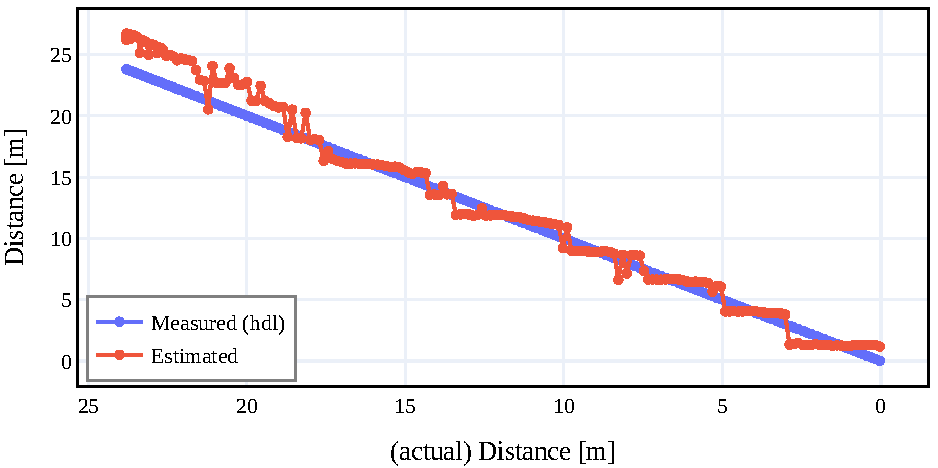
\includegraphics[width=.9\linewidth]{lidar_distance_eval.pdf}
        \caption{Distance to the ramp}
        \label{fig:lidar_distance_eval}
    \end{subfigure}
    
    \begin{subfigure}{1\textwidth}
        \centering
        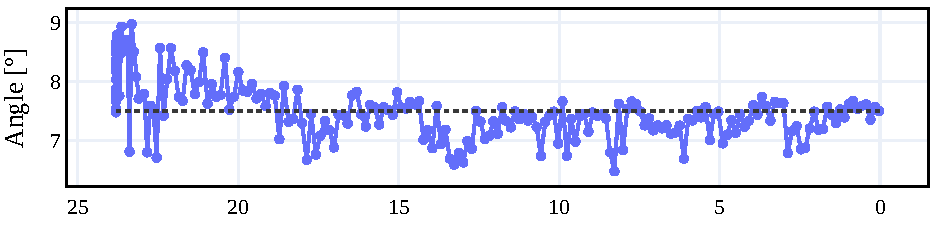
\includegraphics[width=.9\linewidth]{lidar_angle_eval.pdf}
        \caption{Angle of the ramp}
        \label{fig:lidar_angle_eval}
    \end{subfigure}
    
    \begin{subfigure}{1\textwidth}
        \centering
        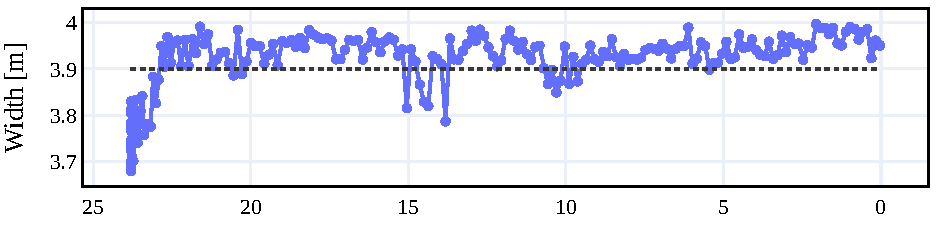
\includegraphics[width=.9\linewidth]{lidar_width_eval.pdf}
        \caption{Width of the ramp}
        \label{fig:lidar_width_eval}
    \end{subfigure}
    
    \begin{subfigure}{1\textwidth}
        \centering
        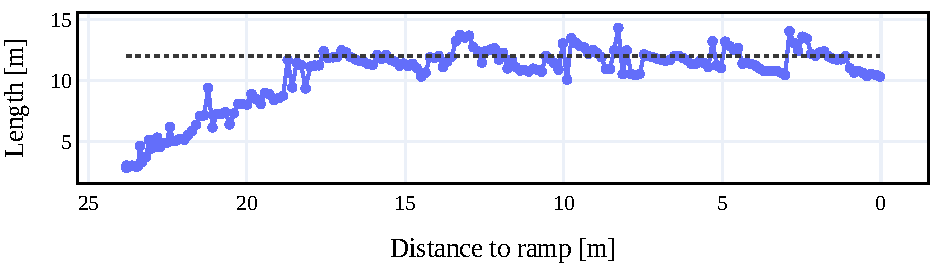
\includegraphics[width=.9\linewidth]{lidar_length_eval.pdf}
        \caption{Length of the ramp}
        \label{fig:lidar_length_eval}
    \end{subfigure}
    \caption[Estimation of ramp properties at different distances]{Estimated ramp properties and tracking of the distance to the ramp at different distances to the ramp.}
    \label{fig:lidar_eval}
\end{figure}
\begin{figure}[htbp]
    \centering
    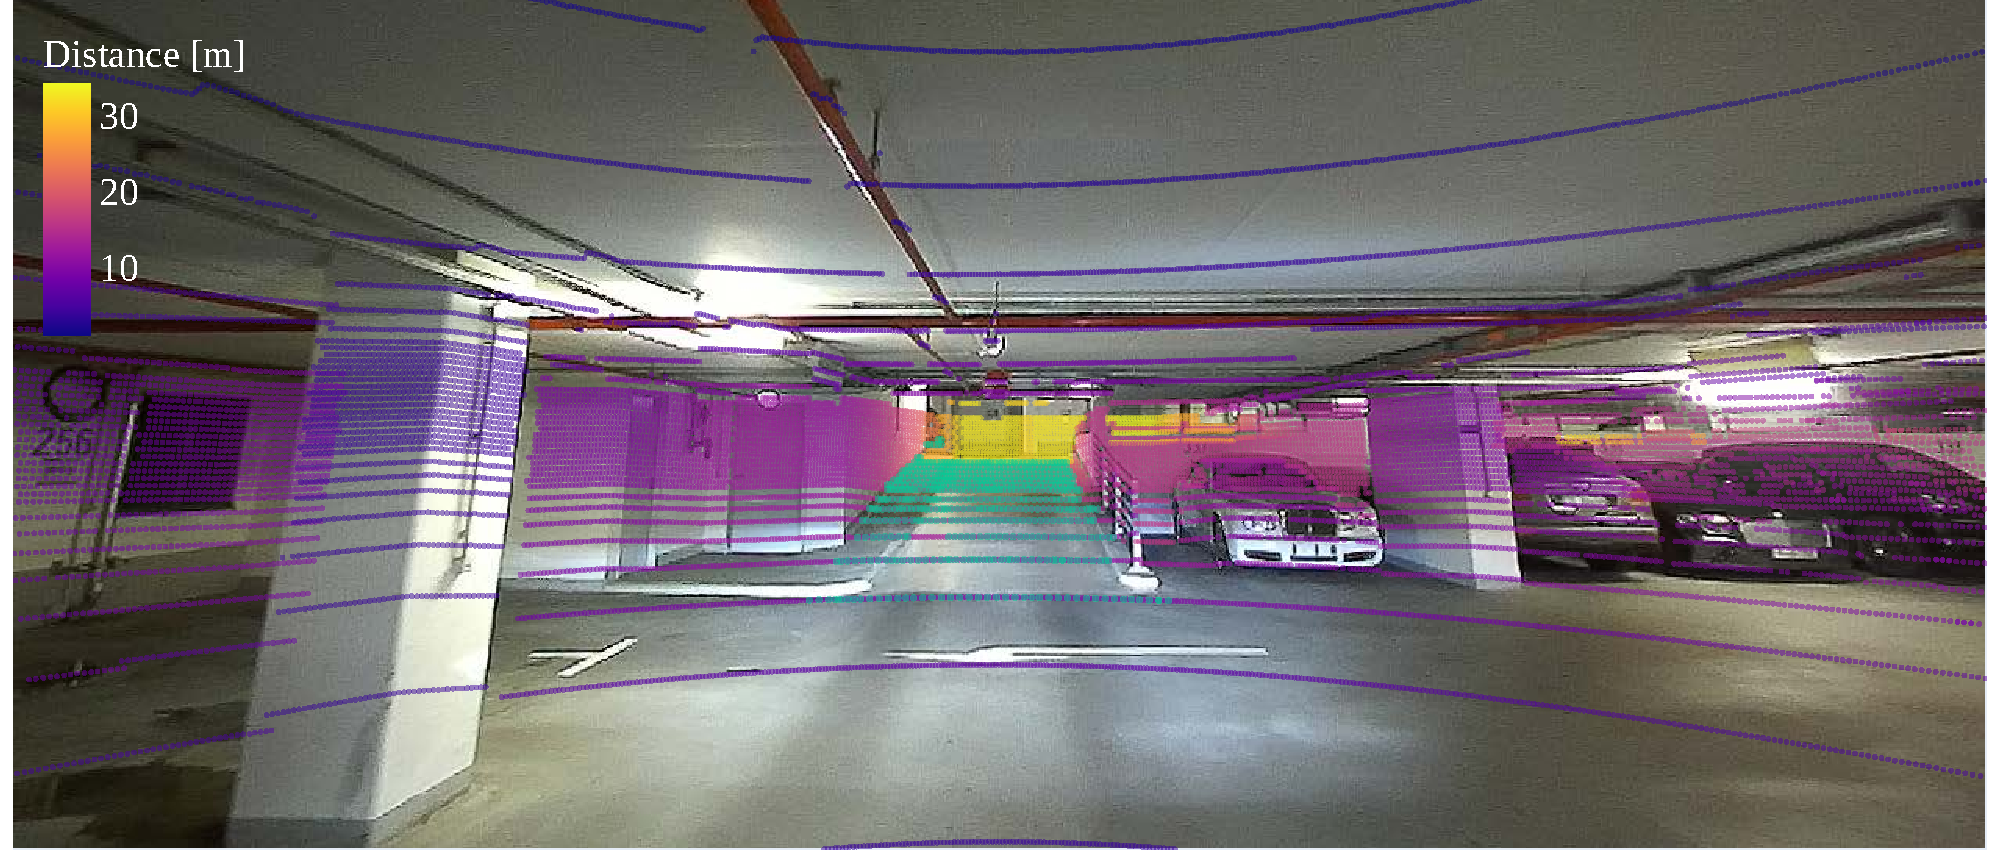
\includegraphics[width=1\linewidth]{points_projection.pdf}
    \caption[2D visualization of the \glsentryshort{lidar} point cloud]{Lidar points projected onto the camera image. The green points were identified as part of a ramp by the algorithm.}
    \label{fig:points_projection}
\end{figure}
A visualization of the detection algorithm can be seen in \cref{fig:points_projection}.
Here, the 3D point cloud generated by the \gls{lidar} is projected onto the 2D camera image.
The quality of the projection depends on the accuracy of the measured translation and orientation difference between both sensors.
It can be seen that it is not perfect, e.g. the points do not quite match the camera image at the left pillar or the pipe on the ceiling.
Nonetheless, it gives a good indication of what the \gls{lidar} actually sees.
The coloring of the point indicates the distance from the car to the points.
Objects far away are marked by yellow points and nearby objects by blue points.
The green points were identified as part of the ramp by the algorithm.
It mostly fits the actual ramp very well.
The previously mentioned problem of the vertical resolution is clearly visible here.
While the density of the laser lines is sufficient in the ramp region, the start of the ramp and especially the ground is covered by very few lines.
This makes the precise tracking of the distance to the ramp difficult.



\section{Camera}
\label{sec:eval_camera}
\subsection{Object Recognition}
The camera was used to detect the ramp and mask the corresponding region in the image.
As described in \cref{sec:performance_measures}, the \gls{map} score is used to evaluate the performance of the neural network.
Since transfer learning is used and the dataset is fairly small, different hyperparameters could be tested.
At first, the different hyperparameters were varied independently of each other to get a rough idea of their influence on the performance.
After this initial test, the best hyperparameters ranges were tested in combination with each other.
In \cref{tab:detection_eval} the \gls{map} scores for different hyperparameters are listed.
LR is the learning rate and SR is the sample rate and determines the number of \gls{roi} proposals, as described in \cref{ssec:training}.\par
\begin{table}[htb]
    \centering
    \caption[Detection evaluation]{Testing of different training hyperparameters and their influence on the \acrshort{ap} score.}
    \label{tab:detection_eval}
    \begin{tabular}{ccccccc}
        \toprule
        % \textbf{Epochs} & \textbf{LR} & \textbf{SR} & \textbf{Box mAP} & \textbf{Mask mAP} \\
        \multicolumn{3}{c}{\textbf{Parameter} } & \multicolumn{2}{c}{\textbf{Scores} }                                                      \\
        \cmidrule(lr){1-3}                       \cmidrule(lr){4-5}
        \textbf{Epochs}                         & \textbf{LR}                          & \textbf{SR} & \textbf{Box mAP} & \textbf{Mask mAP} \\
        \midrule
        1                                       & 0.001                                & 128         & 69.3             & 83.4              \\
        1                                       & 0.001                                & 512         & 84.8             & 85.7              \\
        1                                       & 0.003                                & 128         & 73.3             & 76.8              \\
        1                                       & 0.003                                & 512         & 83.1             & 89.6              \\
        3                                       & 0.001                                & 128         & 77.6             & 90.1              \\
        3                                       & 0.001                                & 512         & 87.3             & 90.8              \\
        3                                       & 0.003                                & 128         & 83.9             & 89.0              \\
        3                                       & 0.003                                & 512         & 84.9             & 87.6              \\
        \bottomrule
    \end{tabular}
\end{table}
Since the configuration using a learning rate of 0.001, sample rate of 512 and 3 epochs achieved the best results, all the following images and calculations were generated using this configuration.
A visualization of the prediction for some example frames when driving straight and from an angle at a ramp can be seen in \cref{fig:camera_prediction_straight} and \cref{fig:camera_prediction_angled} respectively.
In all those cases the detection of the ramp was successful and seems to be fairly accurate.
The annotation inside the image describes how confident the network is about the detection.
All images used for the training and evaluation are colored, but are visualized as grayscale image in this case, to allow for an easier distinction between the segmented region and the background.

\begin{figure}[htb]
    \centering
    \begin{subfigure}{1\textwidth}
        \centering
        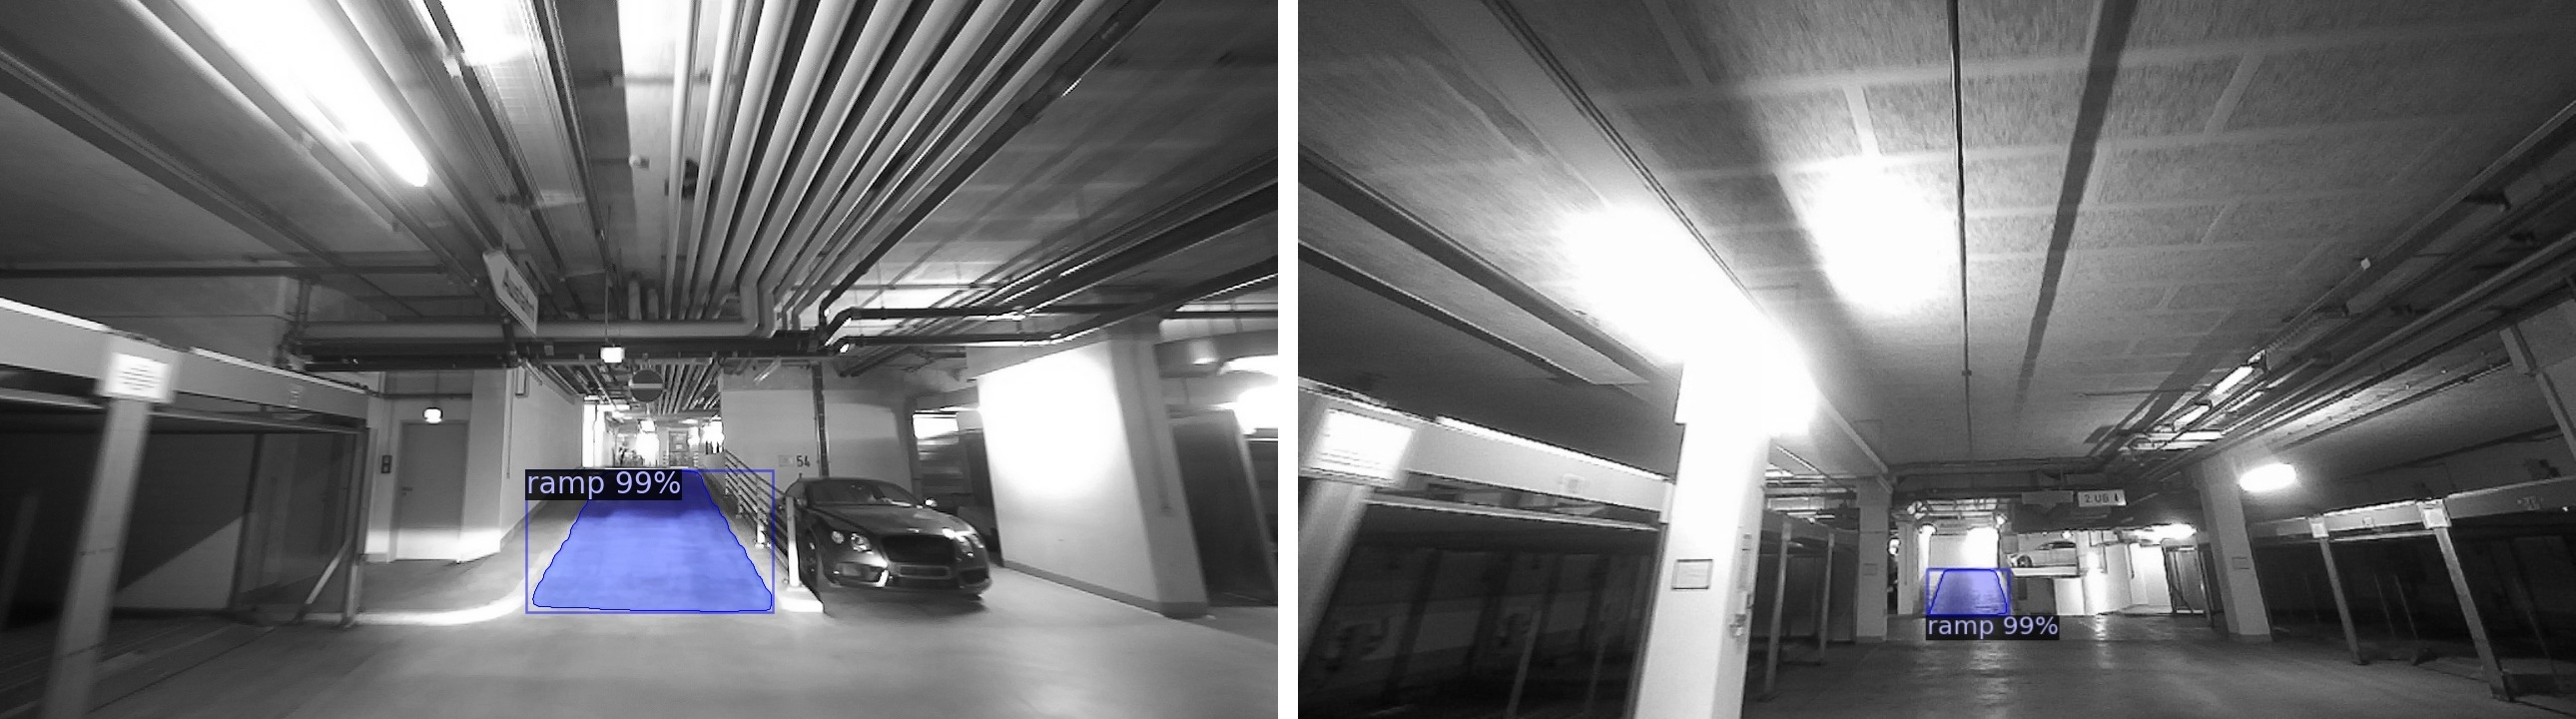
\includegraphics[width=1\linewidth]{camera_prediction_straight}
        \caption{Driving straight at the ramp.}
        \label{fig:camera_prediction_straight}
    \end{subfigure}
    
    % \bigskip
    \begin{subfigure}{1\textwidth}
        \centering
        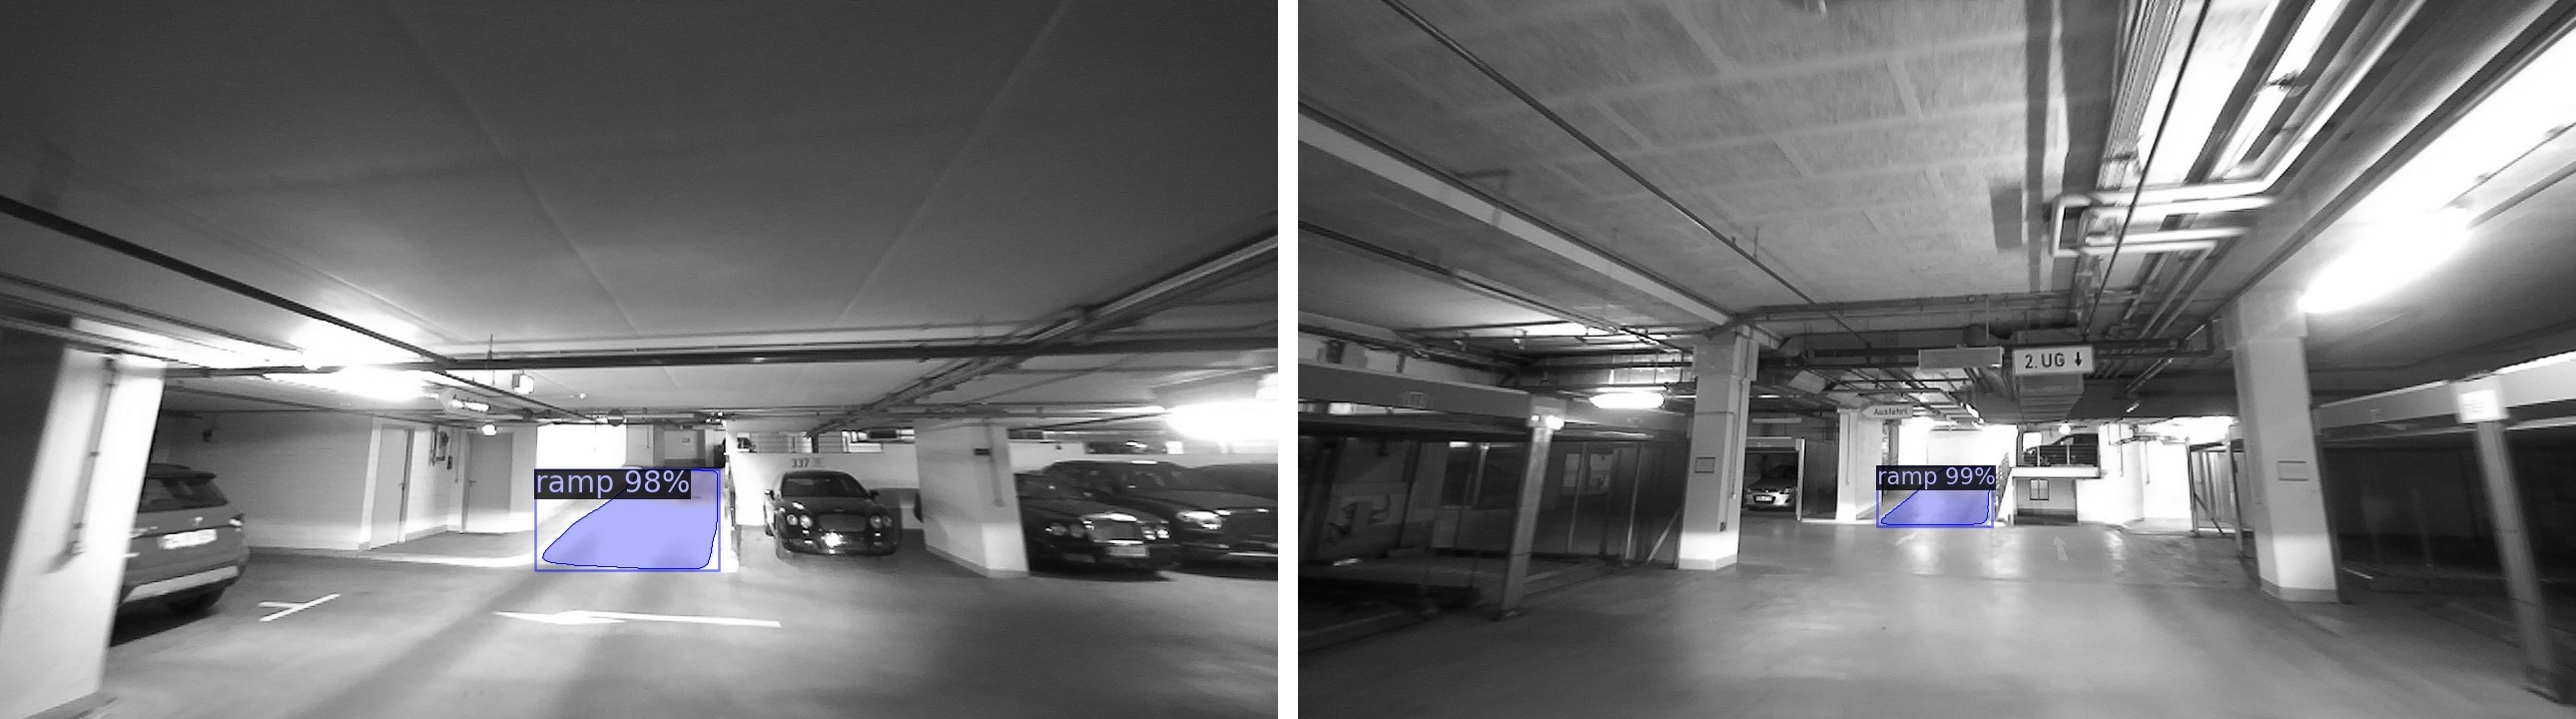
\includegraphics[width=1\linewidth]{camera_prediction_angled}
        \caption{Driving at an angle to the ramp.}
        \label{fig:camera_prediction_angled}
    \end{subfigure}
    \caption[Visualization examples of predicted segmentation masks]{Some examples of the predicted bounding box and mask when driving at a ramp. The class of the object and the confidence score are annotated as well. All those images were not used for the training of the network.}
\end{figure}

\subsection{Point Cloud Extraction}
As described in \cref{ssec:point_cloud_extraction}, the predicted segmentation mask can be used to only extract the points that are part of the ramp from the point cloud.
Different ramp properties can then be calculated from the point cloud.
In a first step, the points must be projected from 3D space into 2D space.
In \cref{fig:points_projection_mask_zed} the projected point cloud of the ZED 2i camera are shown as orange points.
The green points symbolize the points that were detected by the neural network as part of the ramp.
The blue box is the corresponding bounding box.
It can be seen that detection works very well and also only the actual drivable part of the ramp is marked, unlike when just the \gls{lidar} is used (see \cref{fig:points_projection}).
While most of the area is covered by the point cloud, object further away than \SI{20}{\metre} are not detected.
This can be seen in the area above the ramp, which is too far away for the sensor to detect.
But since the car is not far away from the ramp, most of the ramp could be covered by points.\par
This problem is not present, when the point cloud of the \gls{lidar} is used instead.
The projection is shown in \cref{fig:points_projection_mask_lidar}.
It can be seen that the vertical resolution is worse at most opening angles, but the horizontal resolution is better.
This is especially apparent at the beginning of the ramp.
The neural network marked the pixels where the bounding box ends as part of the ramp, but because the \gls{lidar} does not have any points near this line, the nearest marked points are multiple \si{\cm} further away.
This leads to a wrong distance and perhaps length estimation.\par
Projecting the point cloud back into 3D space allows for the calculation of the properties of the ramp.
The results for both sensors are shown in \cref{tab:cloud_extraction_estimation}.
The box method uses the bounding box to extract the points from the point cloud and the mask method uses the mask to extract the points from the point cloud.
The \gls{ransac} algorithm has been applied in both cases to the extracted points, to remove outliers.
The used sensor is written in the subscript of the method name.
Since in the neural network is trained to only detect the drivable part of the ramp, the width had to be measured again.
For the ramp A, the width between the curbs was measured as \SI{2.79}{\metre}.\par
It can be seen that the point cloud generated by the ZED camera produces worse results than the point cloud generated by the lidar.
While it can not be seen very well in \cref{fig:points_projection_mask_zed}, the point cloud was very inaccurate.
The points on the ramp do not build a planar surface, that is why the \gls{ransac} algorithm had trouble to find an optimal plane.
The \gls{lidar} on the other hand produced an accurate point cloud and achieved good results.

\begin{figure}[htb]
    \centering
    \begin{subfigure}{1\textwidth}
        \centering
        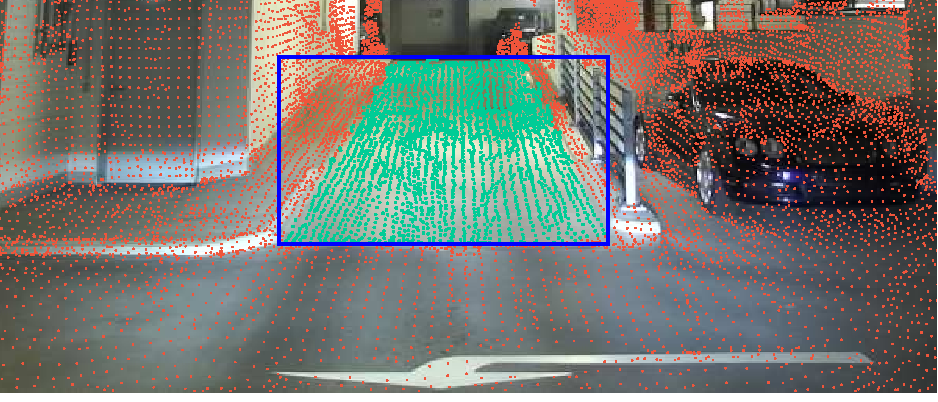
\includegraphics[width=.9\linewidth]{points_projection_mask_zed.pdf}
        \caption{Projection using the by the ZED camera generated point cloud.}
        \label{fig:points_projection_mask_zed}
    \end{subfigure}
    
    % \bigskip
    \begin{subfigure}{1\textwidth}
        \centering
        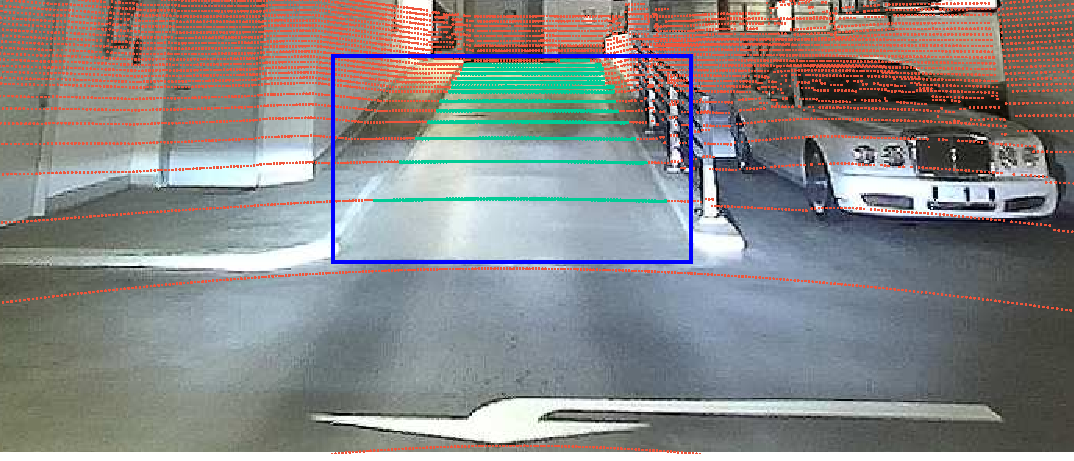
\includegraphics[width=.9\linewidth]{points_projection_mask_lidar.pdf}
        \caption{Projection using the by the \acrshort{lidar} generated point cloud.}
        \label{fig:points_projection_mask_lidar}
    \end{subfigure}
    \caption[Point cloud extraction using the predicted segmentation mask]{Predicted bounding ion of the 3D point cloud onto a 2D image. Using the predicted segmentation mask, the points that lie in the ramp regions can now be extracted from the point cloud.}
\end{figure}
\begin{table}[H]
    \centering
    \caption[Ramp length]{Estimation of different ramp properties using the extracted point cloud.}
    \label{tab:cloud_extraction_estimation}
    \resizebox{\textwidth}{!}{
        \begin{tabular}{lSSSSSS}
            \toprule
            \textbf{Method}            & {\textbf{Angle} [\si{\degree}]} & {\textbf{Error} [\si{\degree}]} & {\textbf{Width} [\si{\metre}]} & {\textbf{Error} [\si{\metre}]} & {\textbf{Length} [\si{\metre}]} & {\textbf{Error} [\si{\metre}]} \\
            \midrule
            $\text{Box}_\text{Zed}$    & 8.84                            & 1.64                            & 3.74                           & 0.95                           & 13.18                           & 1.21                           \\
            $\text{Mask}_\text{Zed}$   & 8.72                            & 1.52                            & 2.53                           & 0.26                           & 12.61                           & 0.64                           \\
            $\text{Box}_\text{LiDAR}$  & 7.78                            & 0.58                            & 5.10                           & 2.31                           & 10.98                           & 0.99                           \\
            $\text{Mask}_\text{LiDAR}$ & 7.64                            & 0.44                            & 2.82                           & 0.03                           & 10.19                           & 1.78                           \\
            \bottomrule
        \end{tabular}
    }
\end{table}
\chapter{Discussion}
\label{ch:Conclusion}
% Do not write long version of imu or lidar acronym again
\glslocalunset{avp}
\glslocalunset{coco}
\glslocalunset{map}
\glslocalunset{imu}
\glslocalunset{lidar}
\glslocalunset{ransac}
\glslocalunset{rcnn}

\section{Summary and Conclusion}
\gls{avp} is a promising application of autonomous driving, in which the car is left in a drop-off zone and drives to its assigned parking spot on its own.
Its use in parking garages is challenging due to the tight turns and limited space.
Ramps are especially difficult to navigate on.
In this thesis different sensors and methods for the detection and classification of ramps in parking garages were developed and evaluated.

Using an \gls{imu}, a ramp could be detected by measuring the tilt of the car.
Different online methods were evaluated, the best results were achieved using a complementary filter, which fuses the accelerometer data and gyroscope data of the \gls{imu}.
By also using the data from the wheel speed sensors, an accurate estimation of the length of the ramp was possible, in addition to the average angle estimation of the ramp.
But overall it can be said that the \gls{imu} data were not very reliable.
The accelerometer data were heavily disturbed when the car did accelerate and the gyroscope data did drift significantly in some cases.

To be able to detect a ramp before entering it, different sensors were used.
At first a \gls{lidar} was tested.
Using the point cloud generated by the \gls{lidar} the planar ramp region could be extracted using the \gls{ransac} algorithm.
The length and width of the ramp could be measured, as well as the average angle of the ramp and the distance of the car to the ramp.
The ramp was successively detected in more than 95\% of the cases, if the distance to the ramp was less than \SI{25}{\metre}.
The \gls{lidar} proofed to be a reliable sensor, but the quality of the results is dependent on the resolution of the \gls{lidar} and the position where it is mounted on the car.
For both the \gls{imu} and \gls{lidar} a novel calibration method was implemented, which automatically transforms the sensor measurements into the coordinate system of the car.

Lastly, a camera was used to detect the ramp.
The object detection was done using the deep learning Mask \gls{rcnn}, which generates a segmentation mask of the object.
An own dataset was created for the training.
Due to the small size, augmented images were added to the dataset and an on the \gls{coco} dataset pretrained network was used.
The network proofed to be able to detect ramps well and achieved great results with an \gls{map} score of over 90\%.
But no quantitative description of the ramp properties was possible using this method.

Lastly the predicted segmentation mask was elevated into 3D space, by projection a 3D point cloud onto an image, removing points outside the mask, and then transforming them back into 3D space.
This was done for the point cloud generated by a stereo camera, and the point cloud of the \gls{lidar}.
This allowed for the accurate detection of the drivable part of the ramp in 3D space, whereas the \gls{lidar} algorithm did not make a distinction between the drivable part and the curb sides.
Also, the ramp properties could now be calculated.
The point cloud of the stereo camera was not as precise as the of the \gls{lidar}, but was easier to project, since no transformation between the camera image and point cloud reference frame system was needed.

Overall it can be said, that using the neural network to detect the ramp in the image and extracting the corresponding points from the \gls{lidar} point cloud, seems to be a very promising method.
The \gls{imu} data are not very reliable, but could be used to further improve the estimation from the other methods.



\section{Future Work}
In this thesis different sensors were used to detect a ramp and measure its properties.
While relatively good results could be achieved, each method could be improved further.
For the \gls{imu} other algorithms such as a Kalman filter could be tested.
Furthermore, the problem of the delay between the wheel speed sensor and \gls{imu} measurements could be investigated.
The same goes for the \gls{lidar}, other algorithms than \gls{ransac} could be tested.
There exist newer algorithms which are more efficient, which means that the downsampling and passthrough filtering could be reduced.
The neural network for the object detection could also be made more robust by using more data, preferably of other environments, in the training.

To further improve the results, the different methods could also be combined.
In this thesis the online implementation of the objection detection was not carried out, this could be done in the future.
Then, the \gls{lidar} point cloud extraction using the instance segmentation prediction could also be properly evaluated.
Another option of sensor fusion would be to use the estimated ramp properties using the \gls{lidar} data and correct them after driving on the ramp using the \gls{imu} data.
Also, the distance tracking to the ramp using the \gls{lidar} could be improved, by fusing the estimation from the \gls{lidar} data with the wheel speed measurements.

For the evaluation of the different methods the \gls{lidar} data was used, which is subject to error.
Additionally, the testing in a more controlled environment would be useful.
This could be done in a simulated environment, e.g. in \texttt{CARLA}~\footnote{\url{https://github.com/carla-simulator/carla}}~\cite{Dosovitskiy2017}.
Furthermore, testing the system in other environments could be useful.

Another potential future task would be to use the implemented methods to create a meta map of the environment.
If a map is created, e.g. using the \gls{lidar} and the \texttt{hdl\_slam} library, the location of the ramp could be labeled in the map, together with the properties of the ramp.






%\pagestyle{fancy}
\chapter{Appendix}
\label{ch:Appendix}

Code Example
\begin{lstlisting}[language=Python]
	import numpy as np
	
	def incmatrix(genl1,genl2):
	m = len(genl1)
	n = len(genl2)
	M = None #to become the incidence matrix
	VT = np.zeros((n*m,1), int)  #dummy variable
	
	#compute the bitwise xor matrix
	M1 = bitxormatrix(genl1)
	M2 = np.triu(bitxormatrix(genl2),1) 
	
	for i in range(m-1):
	for j in range(i+1, m):
	[r,c] = np.where(M2 == M1[i,j])
	for k in range(len(r)):
	VT[(i)*n + r[k]] = 1;
	VT[(i)*n + c[k]] = 1;
	VT[(j)*n + r[k]] = 1;
	VT[(j)*n + c[k]] = 1;
	
	if M is None:
	M = np.copy(VT)
	else:
	M = np.concatenate((M, VT), 1)
	
	VT = np.zeros((n*m,1), int)
	
	return M
\end{lstlisting}
vs
\bibliographystyle{plain}
\bibliography{References/references.bib}
\end{document}
